\documentclass[12pt,spanish,fleqn,openany,letterpaper,pagesize]{scrbook}

%\usepackage[ansinew]{inputenc}
\usepackage[spanish]{babel}
\usepackage[utf8]{inputenc}

\usepackage{fancyhdr}
\usepackage{epsfig}
\usepackage{epic}
\usepackage{eepic}
\usepackage{amsmath}
\usepackage{threeparttable}
\usepackage{amscd}
\usepackage{here}
\usepackage{graphicx}
\usepackage{lscape}
\usepackage{tabularx}
\usepackage{subfigure}
\usepackage{longtable}
\usepackage{bm}


\usepackage{rotating} %Para rotar texto, objetos y tablas seite. No se ve en DVI solo en PS. Seite 328 Hundebuch
                        %se usa junto con \rotate, \sidewidestable ....


\renewcommand{\theequation}{\thechapter-\arabic{equation}}
\renewcommand{\thefigure}{\textbf{\thechapter-\arabic{figure}}}
\renewcommand{\thetable}{\textbf{\thechapter-\arabic{table}}}


\pagestyle{fancyplain}%\addtolength{\headwidth}{\marginparwidth}
\textheight22.5cm \topmargin0cm \textwidth16.5cm
\oddsidemargin0.5cm \evensidemargin-0.5cm%
\renewcommand{\chaptermark}[1]{\markboth{\thechapter\; #1}{}}
\renewcommand{\sectionmark}[1]{\markright{\thesection\; #1}}
\lhead[\fancyplain{}{\thepage}]{\fancyplain{}{\rightmark}}
\rhead[\fancyplain{}{\leftmark}]{\fancyplain{}{\thepage}}
\fancyfoot{}
\thispagestyle{fancy}%


\addtolength{\headwidth}{0cm}
\unitlength1mm %Define la unidad LE para Figuras
\mathindent0cm %Define la distancia de las formulas al texto,  fleqn las descentra
\marginparwidth0cm
\parindent0cm %Define la distancia de la primera linea de un parrafo a la margen

%Para tablas,  redefine el backschlash en tablas donde se define la posici\'{o}n del texto en las
%casillas (con \centering \raggedright o \raggedleft)
\newcommand{\PreserveBackslash}[1]{\let\temp=\\#1\let\\=\temp}
\let\PBS=\PreserveBackslash

%Espacio entre lineas
\renewcommand{\baselinestretch}{1.1}

%Neuer Befehl f\"{u}r die Tabelle Eigenschaften der Aktivkohlen
\newcommand{\arr}[1]{\raisebox{1.5ex}[0cm][0cm]{#1}}

%Neue Kommandos
\usepackage{Befehle}


%Trennungsliste
\hyphenation {Reaktor-ab-me-ssun-gen Gas-zu-sa-mmen-set-zung
Raum-gesch-win-dig-keit Durch-fluss Stick-stoff-gemisch
Ad-sorp-tions-tem-pe-ra-tur Klein-schmidt
Kohlen-stoff-Mole-kular-siebe Py-rolysat-aus-beu-te
Trans-port-vor-gan-ge}
%\includeonly{Kap1/Kap1,Kap2/Kap2}
\begin{document}
\pagenumbering{roman}
%\newpage
%\setcounter{page}{1}
\begin{center}
\begin{figure}
\centering%

\epsfig{file=HojaTitulo/EscudoUN.eps,scale=1}%
\end{figure}
\thispagestyle{empty} \vspace*{2.0cm} \textbf{\huge
Din\'amica estelar y perfiles gal\'acticos de lentes gravitacionales}\\[6.0cm]
%T\'{\i}tulo de la tesis  o trabajo de investigaci\'{o}n}\\[6.0cm]
\Large\textbf{Andr\'es Felipe Granados Cruz}\\[6.0cm]
\small Universidad Nacional de Colombia\\
Facultad, Departamento de F\'isica\\
Ciudad, Colombia\\
2018\\
\end{center}

\newpage{\pagestyle{empty}\cleardoublepage}

\newpage
\begin{center}
\thispagestyle{empty} \vspace*{0cm} \textbf{\huge
Din\'amica estelar y perfiles gal\'acticos de lentes gravitacionales}\\[3.0cm]
\Large\textbf{Andr\'es Felipe Granados Cruz}\\[3.0cm]
\small Tesis o trabajo de grado presentada(o) como requisito parcial para optar al
t\'{\i}tulo de:\\
\textbf{F\'isico}\\[2.5cm]
Director(a):\\
Ph.D. Leonardo Castañeda\\[2.0cm]
L\'{\i}nea de Investigaci\'{o}n:\\
Dinámica galáctica\\
Grupo de Investigaci\'{o}n:\\
Astronomía Galáctica, Gravitación y Cosmología\\[2.5cm]
Universidad Nacional de Colombia\\
Facultad de Ciencias, Departamento de Física\\
Bogotá D.C., Colombia\\
2018\\
\end{center}

\newpage{\pagestyle{empty}\cleardoublepage}

\newpage
\thispagestyle{empty} \textbf{}\normalsize
\\\\\\%
\textbf{(Dedicatoria o un lema)}\\[4.0cm]

\begin{flushright}
\begin{minipage}{8cm}
    \noindent
        \small
        Su uso es opcional y cada autor podr\'{a} determinar la distribuci\'{o}n del texto en la p\'{a}gina, se sugiere esta presentaci\'{o}n. En ella el autor dedica su trabajo en forma especial a personas y/o entidades.\\[1.0cm]\\
        Por ejemplo:\\[1.0cm]
        A mis padres\\[1.0cm]\\
        o\\[1.0cm]
        La preocupaci\'{o}n por el hombre y su destino siempre debe ser el
        inter\'{e}s primordial de todo esfuerzo t\'{e}cnico. Nunca olvides esto
        entre tus diagramas y ecuaciones.\\\\
        Albert Einstein\\
\end{minipage}
\end{flushright}

\newpage{\pagestyle{empty}\cleardoublepage}

\newpage
\thispagestyle{empty} \textbf{}\normalsize
\\\\\\%
\textbf{\LARGE Agradecimientos}
\addcontentsline{toc}{chapter}{\numberline{}Agradecimientos}\\\\
Esta secci\'{o}n es opcional, en ella el autor agradece a las personas o instituciones que colaboraron en la realizaci\'{o}n de la tesis  o trabajo de investigaci\'{o}n. Si se incluye esta secci\'{o}n, deben aparecer los nombres completos, los cargos y su aporte al documento.\\

\newpage{\pagestyle{empty}\cleardoublepage}

\newpage
\textbf{\LARGE Resumen}
\addcontentsline{toc}{chapter}{\numberline{}Resumen}\\\\
Un sistema estelar puede ser descrito por una función de distribución de partículas que no colisionan, en la ecuación de Vlasov que relaciona el potencial gravitacional del sistema con su función de distribución. El primer y segundo momentos de la función de distribución da cuenta de la velocidad y del tensor de dispersión de velocidades que caracteriza la cinemática como observables del sistema y su relación con la dinámica está dada por las ecuaciones de Jeans. Se revisan los métodos de expansión gaussiano del potencial gravitacional y el modelamiento axialmente simétrico de las ecuaciones de Jeans con parámetro de anisotropía del elipsoide de velocidades. Por otra parte la curva de rotación galáctica permite obtener de manera directa la distribución de materia apoyado por fuerte evidencia observacional gracias al método de descomposición del potencial gravitacional en uno de bulbo, disco estelar y de materia oscura. La descripción que viene de la dinámica estelar es contrastado con el resultado que proviene del efecto de lente gravitacional. Éste último surge de la deflexión a la que es sometida la luz de un objeto fuente lejano, por efecto de la gravedad de otro objeto interpuesto entre la fuente y el observador, denominado lente. Los modelos de lente permiten obtener la posición en el cielo del objeto fuente mediante las posiciones de sus imágenes producidas por la lente y del ángulo de deflexión. El ángulo de deflexión contiene la información del potencial gravitacional deflector y así mismo de la distribución de materia mediante la ecuación de Poisson. El objeto de estudio es el sistema lente+galaxia espiral SDSS J1331+3628 del cual se realizó las deducciones para obtener su distribución de materia por el ajuste de la curva de rotación de la galaxia y por medio de un modelo de lente independiente de escala.\\

El resumen es una presentaci\'{o}n abreviada y precisa (la NTC 1486 de 2008 recomienda revisar la norma ISO 214 de 1976). Se debe usar una extensi\'{o}n m\'{a}xima de 12 renglones. Se recomienda que este resumen sea anal\'{\i}tico, es decir, que sea completo, con informaci\'{o}n cuantitativa y cualitativa, generalmente incluyendo los siguientes aspectos: objetivos, dise\~{n}o, lugar y circunstancias, pacientes (u objetivo del estudio), intervenci\'{o}n, mediciones y principales resultados, y conclusiones. Al final del resumen se deben usar palabras claves tomadas del texto (m\'{\i}nimo 3 y m\'{a}ximo 7 palabras), las cuales permiten la recuperaci\'{o}n de la informaci\'{o}n.\\

\textbf{\small Palabras clave: función de distribución, ecuación de Vlasov, ecuaciones de Jeans, galaxias: cinemática y dinámica, anisotropía, elipsoide de velocidades, lente gravitacional, bulbo estelar, materia oscura  }.\\


\textbf{\LARGE Abstract}\\\\
Es el mismo resumen pero traducido al ingl\'{e}s. Se debe usar una extensi\'{o}n m\'{a}xima de 12 renglones. Al final del Abstract se deben traducir las anteriores palabras claves tomadas del texto (m\'{\i}nimo 3 y m\'{a}ximo 7 palabras), llamadas keywords. Es posible incluir el resumen en otro idioma diferente al espa\~{n}ol o al ingl\'{e}s, si se considera como importante dentro del tema tratado en la investigaci\'{o}n, por ejemplo: un trabajo dedicado a problemas ling\"{u}\'{\i}sticos del mandar\'{\i}n seguramente estar\'{\i}a mejor con un resumen en mandar\'{\i}n.\\[2.0cm]
\textbf{\small Keywords: palabras clave en ingl\'{e}s(m\'{a}ximo 10 palabras, preferiblemente seleccionadas de las listas internacionales que permitan el indizado cruzado)}\\

\renewcommand{\tablename}{\textbf{Tabla}}
\renewcommand{\figurename}{\textbf{Figura}}
\renewcommand{\listtablename}{Lista de Tablas}
\renewcommand{\listfigurename}{Lista de Figuras}
\renewcommand{\contentsname}{Contenido}


%\newcommand{\clearemptydoublepage}{\newpage{\pagestyle{empty}\cleardoublepage}}
\tableofcontents
\chapter*{Lista de s\'{\i}mbolos}
\addcontentsline{toc}{chapter}{\numberline{}Lista de s\'{\i}mbolos}
Esta secci\'{o}n es opcional, dado que existen disciplinas que no manejan s\'{\i}mbolos y/o abreviaturas.\\

Se incluyen s\'{\i}mbolos generales (con letras latinas y griegas), sub\'{\i}ndices, super\'{\i}ndices y abreviaturas (incluir s\'{o}lo las clases de s\'{\i}mbolos que se utilicen). Cada una de estas listas debe estar ubicada en orden alfab\'{e}tico de acuerdo con la primera letra del s\'{\i}mbolo.
\section*{S\'{\i}mbolos con letras latinas}
 \label{simbolos}
 \renewcommand{\arraystretch}{1.3}
%\begin{longtable}[l]{*{4}{>{$}l<{$}}p{9cm}}
\begin{longtable}[l]{>{$}l<{$}l>{$}l<{$}>{$}l<{$}}
%\begin{tabular}
\textbf{S\'{\i}mbolo}&\textbf{T\'{e}rmino}&\textbf{Unidad SI}&\textbf{Definici\'{o}n}\\[0.5ex]\hline
\endfirsthead%
\textbf{S\'{\i}mbolo}&\textbf{T\'{e}rmino}&\textbf{Unidad SI}&\textbf{Definici\'{o}n}\\[0.5ex]\hline
\endhead%
      A              &\'{A}rea                                   &\text{m}^{2}                         &\int\int dxdy\\%
      A_{\text{BET}} &\'{A}rea interna del s\'{o}lido                &\frac{\text{m}^{2}}{\text{g}}        &\text{ver DIN ISO 9277}\\%
      A_{\text{g}}   &\'{A}rea transversal de la fase gaseosa    &\text{m}^{2}                         &\text{Ec...}\\%
      A_{\text{s}}   &\'{A}rea transversal de la carga a granel  &\text{m}^{2}                         &\text{Ec...}\\%
      a              &Coeficiente                            &1                                    &\text{Ec...}\\%
      a              &Contenido de ceniza                    &1                                    &\frac{m_{\text{ceniza}}}{m_{\text{bm,0}}}\\%
      c              &Contenido de carbono                   &1                                    &\frac{m_{\text{C}}}{m}\\%
      c              &Longitud de la cuerda                  &\text{m}                             &\text{Figura...}\\
      c              &Concentraci\'{o}n de la cantidad de materia&\frac{\text{mol}}{\text{m}^{3}}      &\frac{n}{V}\\%
      D              &Di\'{a}metro                               &\text{m}                             &\\%
      E_{\text{A}}   &Energ\'{\i}a de activaci\'{o}n                  &\frac{\text{kJ}}{\text{mol}}         &\text{Ec....}\\%
      F              &Fracci\'{o}n de materia vol\'{a}til            &1                                    &\text{ver DIN 51720}\\%
      Fr             &N\'{u}mero de Froude                       &1                                    &\frac{\omega^{2}R}{g_{\text{0}}}\\%
      \overrightarrow{g}&Aceleraci\'{o}n de la gravedad          &\frac{\text{m}}{\text{s}^{2}}        &\frac{d^{2}\overrightarrow{r}}{dt^{2}}\\%
      H              &Entalp\'{\i}a                               &\text{J}                             &U+PV\\%
      H_{\text{o}}   &Poder calor\'{\i}fico superior              &\frac{\text{MJ}}{\text{kg}}          &\text{ver DIN 51857}\\%
      h              &Contenido de hidr\'{o}geno                 &1                                    &\frac{m_{\text{H}}}{m}\\%
      K              &Coeficiente de equilibrio              &1                                    &\text{Ec...}\\%
      L              &Longitud                               &\text{m}                             &DF\\%
      L              &Longitud del reactor                   &\text{m}                             &\text{Figura...}\\%
      m              &Masa                                   &\text{kg}                            &DF\\%
      \dot{m}        &Flujo de masa                          &\frac{\text{kg}}{\text{s}}           &\frac{m}{t}\\%
      n              &Velocidad de rotaci\'{o}n                  &\frac{\text{1}}{\text{s}}            &\frac{\omega}{2\pi}\\%
      n              &Cantidad de materia                    &\text{mol}                           &DF\\%
      P              &Presi\'{o}n                                &\text{Pa}                            &\frac{\vec{F}\cdot\vec{n}}{A}\\%
      Q              &Calor                                  &\text{kJ}                            &\text{1. $LT$}\\%
      T              &Temperatura                            &\text{K}                             &DF\\%
      t              &Tiempo                                 &\text{s}                             &DF\\%
      x_{\text{i}}   &Fracci\'{o}n de la cantidad de materia     &1                                    &\frac{n_{\text{i}}}{n}\\%
      V              &Volumen                                &\text{m}^{3}                         &\int{dr^{3}}\\%
      \vec{u}        &Velocidad                              &\frac{\text{m}}{\text{s}}            &(\frac{dr}{dt},r\frac{d\upsilon}{dt},\frac{dz}{dt})\\%
      w_{\text{i}}   &Fracci\'{o}n en masa del componente i      &1                                    &\frac{m_{\text{i}}}{m_{\text{0}}}\\%
      w_{\text{w,i}} &Contenido de humedad de la sustancia i &1                                    &\frac{m_{\text{\wasser}}}{m_{\text{i,0}}}\\%
      Z              &Factor de gases reales                 &1                                    &\frac{pv}{RT}\\%
\end{longtable}
\vspace{5ex}
\section*{S\'{\i}mbolos con letras griegas}

\begin{longtable}[l]{>{$}l<{$}l>{$}l<{$}>{$}l<{$}}
\textbf{S\'{\i}mbolo}&\textbf{T\'{e}rmino}&\textbf{Unidad SI}&\textbf{Definici\'{o}n}\\[0.5ex] \hline%
\endfirsthead%
\textbf{S\'{\i}mbolo}&\textbf{T\'{e}rmino}&\textbf{Unidad SI}&\textbf{Definici\'{o}n}\\[0.5ex] \hline%
\endhead%
\renewcommand{\arraystretch}{1.3}
 \label{simbolosg}
     \alpha_{\text{BET}}  &Factor de superficie                  &\frac{\text{m}^{2}}{\text{g}}   &(w_{\text{F,waf}})(A_{\text{BET}})\\%
     \beta_{\text{i}}     &Grado de formaci\'{o}n del componente i   &1                               &\frac{m_{\text{i}}}{m_{\text{bm,0}}}\\%
     \gamma               &Wandhaftreibwinkel (Stahlblech)       &1                               &\text{Secci\'{o}n...}\\
     \epsilon             &Porosidad de la part\'{\i}cula             &1                               &1-\frac{\rho_{\text{s}}}{\rho_{\text{w}}}\\%
     \eta                 &mittlere Bettneigungswinkel (St\"{u}rzen) &1                               &\text{Figura...}\\%
     \theta               &\'{A}ngulo de inclinaci\'{o}n de la cama      &1                               &\text{Figura...}\\
     \theta_{\text{O}}    &\'{A}ngulo superior de avalancha          &1                               &\text{Figura...}\\
     \theta_{\text{U}}    &\'{A}ngulo inferior de avalancha          &1                               &\text{Figura...}\\
     \kappa               &Velocidad de calentamientoe           &\frac{\text{K}}{\text{s}}       &\frac{dT}{dt}\\%
     \nu                  &Coeficiente estequiom\'{e}trico           &1                               &\text{ver DIN 13345}\\%
     \rho_{\text{b}}      &Densidad a granel                     &\frac{\text{kg}}{\text{m}^{3}}  &\frac{m_{\text{S}}}{V_{\text{S}}}\;(\text{Secci\'{o}n...})\\
     \rho_{\text{s}}      &Densidad aparente                     &\frac{\text{kg}}{\text{m}^{3}}  &\frac{m_{\text{F}}}{V_{\text{P}}}\;(\text{Secci\'{o}n...})\\
     \rho_{\text{w}}      &Densidad verdadera                    &\frac{\text{kg}}{\text{m}^{3}}  &\frac{m_{\text{F}}}{V_{\text{F}}}\;(\text{Secci\'{o}n...})\\
     \tau                 &Tiempo adimensional                   &1                               &\text{Ec....}\\%
     \Phi_{\text{V}}      &Flujo volum\'{e}trico                     &\frac{\text{m}^{3}}{\text{s}}   &\frac{\Delta V}{\Delta t}\\
     \omega               &Velocidad angular                     &\frac{1}{\text{s}}              &\frac{d\upsilon}{dt}\\

\end{longtable}


\section*{Sub\'{\i}ndices}
\begin{longtable}[l]{>{}l<{}l}
  \textbf{Sub\'{\i}ndice} & \textbf{T\'{e}rmino} \\[0.5ex] \hline%
  \endfirsthead%
  \textbf{Sub\'{\i}ndice} & \textbf{T\'{e}rmino} \\[0.5ex] \hline%
  \endhead%
\renewcommand{\arraystretch}{1.4}\label{simbolosg}

 bm&materia org\'{a}nica\\%
 DR&Dubinin-Radushkevich\\%
 E&Experimental\\%
 g&Fase gaseosa\\%
 k&Condensado\\%
 Ma&Macroporos\\%
 P&Part\'{\i}cula\\%
 p&Poro\\%
 p&Pirolizado\\%
 R&Reacci\'{o}n\\%
 t&Total\\%
 wf&Libre de agua\\%
 waf&Libre de agua y de ceniza\\%
 0&Estado de referencia\\%

\end{longtable}


\setlength{\extrarowheight}{0pt}


\section*{Super\'{\i}ndices}
\begin{longtable}[l]{>{}l<{}l}
  \textbf{Super\'{\i}ndice} & \textbf{T\'{e}rmino} \\[0.5ex] \hline%
  \endfirsthead%
  \textbf{Super\'{\i}ndice} & \textbf{T\'{e}rmino} \\[0.5ex] \hline%
  \endhead%
\renewcommand{\arraystretch}{1.4}\label{simbolosg}

 n &Coeficiente x\\%



\end{longtable}


\setlength{\extrarowheight}{0pt}


\section*{Abreviaturas}
\begin{longtable}[l]{>{}l<{}l}
  \textbf{Abreviatura} & \textbf{T\'{e}rmino} \\[0.5ex] \hline%
  \endfirsthead%
  \textbf{Abreviatura} & \textbf{T\'{e}rmino} \\[0.5ex] \hline%
  \endhead%
\renewcommand{\arraystretch}{1.4}\label{simbolosg}
 1.$LT$&Primera ley de la termodin\'{a}mica\\%
 $DF$    &Dimensi\'{o}n fundamental\\%
 $RFF$   &Racimos de fruta fresca\\%

\end{longtable}


\setlength{\extrarowheight}{0pt}
%\include{Resumen}%\newcommand{\clearemptydoublepage}{\newpage{\pagestyle{empty}\cleardoublepage}}
\pagenumbering{arabic}
\chapter{Introducci\'{o}n}

En 1914 Vesto Slipher descubrió que las galaxias espirales rotan. Detectó líneas de absorción inclinadas en el espectro  de las galaxias  M31 y Sobrero \cite{Slipher1914}. Después, Jan Oort en 1932 encontró por primera vez que debe haber tres veces tanta masa como es observado la luz visible, mientras estudiaba movimientos estelares sobre el plano de la Via Láctea. Este descubrimiento le sugirió incluir componentes de medio interestelar no detectado para explicar la masa faltante en este sistema. Observaciones similares para las partes externas de NGC3115 mostró que la razón masa a luz es aproximadamente dos órdenes  de magnitud mayor que en la vecindad solar \cite{Oort40} como evidencia  de materia no visible. Ésto es conocido como el problema de la `masa faltante'; esto es, la masa contenida en objetos brillantes de una región definida en el espacio no corresponde a su masa dinámica que podemos conocer por las interacciones gravitacionales.\\

La razón masa a luz $\Upsilon = M/L$ es una cantidad que describe cuánta masa es una fracción de la luz expresado en unidades solares ($\Upsilon_\odot = \textrm{M}_\odot\textrm{L}_\odot^{-1}$). Esta cantidad ha sido la principal herramienta para investigar el problema de la `masa faltante' en sistemas estelares como la  Vía Lactea, galaxias externas y cúmulos de galaxias.\\

Han surgido algunas explicaciones del problema de la `masa faltante'. H. Babcock en 1939 encontró que la curva de rotación es aproximadamente plana en la periferia  de la galaxia M31 en lugar de la caída Kepleriana dada la disminución de la luminosidad (predicha por el perfil de luminosidad) \cite{Babcock1939}. Él concluyó que la razón masa-luz no debe ser constante en el radio galáctico, pero debe incrementar. Él sugirió dos explicaciones para este fenómeno: la absorción de luz debe incrementar en las partes externas de la galaxia, o se requiere una modificación a la dinámica Newtoniana \cite{Sanders}. \\

Los descubrimientos publicados por Fritz Zwicky \cite{Z33, Z37} sugirieron la existencia de `materia no visible' o materia oscura en sus resultados usando el teorema del virial a las velocidades de galaxias en el cúmulo Coma. Zwicky midió las velocidades radiales de galaxias en el cúmulo, y estimó su masa y por lo tanto la masa promedio de la galaxia. Entonces comparando su valor con la luminosidad, él obtuvo la razón masa a luz de galaxias en el cúmulo $\Upsilon = M/L = 500 \Upsilon_\odot$ sugiriendo que la mayor contribución es materia oscura en el cúmulo. Después, en 1970 Vera Rubin primero reveló una evidencia observacional de materia oscura en la galaxia M31. Ella se dió cuenta que la velocidad circular se vuelve constante en regiones externas de la galaxia basado en su curva de rotación de 67 espectros  H\textsc{ii}  entre un rango en el radio galáctico de (3-24 kpc) \cite{R70}.\\

La curva de rotación de galaxias tipo disco en el principal observable cinemático que permite estudiar propiedades dinámicas de sus estrellas y gas interestelar, en adición a la estructura, procesos de formación e la galaxia \cite{S01}. La forma de las curvas de rotación se relaciona con la morfología de galaxias espirales \cite{R80} buscando una curva de rotación universal dependiendo solo de la luminosidad de la galaxia \cite{P96}, y no solo de la luminosidad sino de una familia multi-parámetro tal como tipo morfológico, la forma de la distribución de luz y otras propiedades ópticas\cite{N07}.\\

La distribución de masa en una componente de una galaxia puede ser estimada por la suposición que la razón masa a luz es constante. Dado que la luminosidad de la galaxia es un observable astrofísico, puede ser obtenido un perfil de luminosidad de una componente y por lo tanto inferir su distribución de masa. Entonces es posible encontrar una curva de rotación para cada contribución de masa y derivar cantidades interesantes como la relación de masas bulbo a disco o disco a materia oscura, o igualmente interesante la extensión radial de cada componente de masa. El modelamiento de la curva de rotación usando descomposición de masa is ampliamente usado en estudios recientes. Esto evidencia la influencia de todas las contribuciones de masa en cada posición, del núcleo hasta décadas en el radio galáctico.\\


\begin{figure}
  \centering
    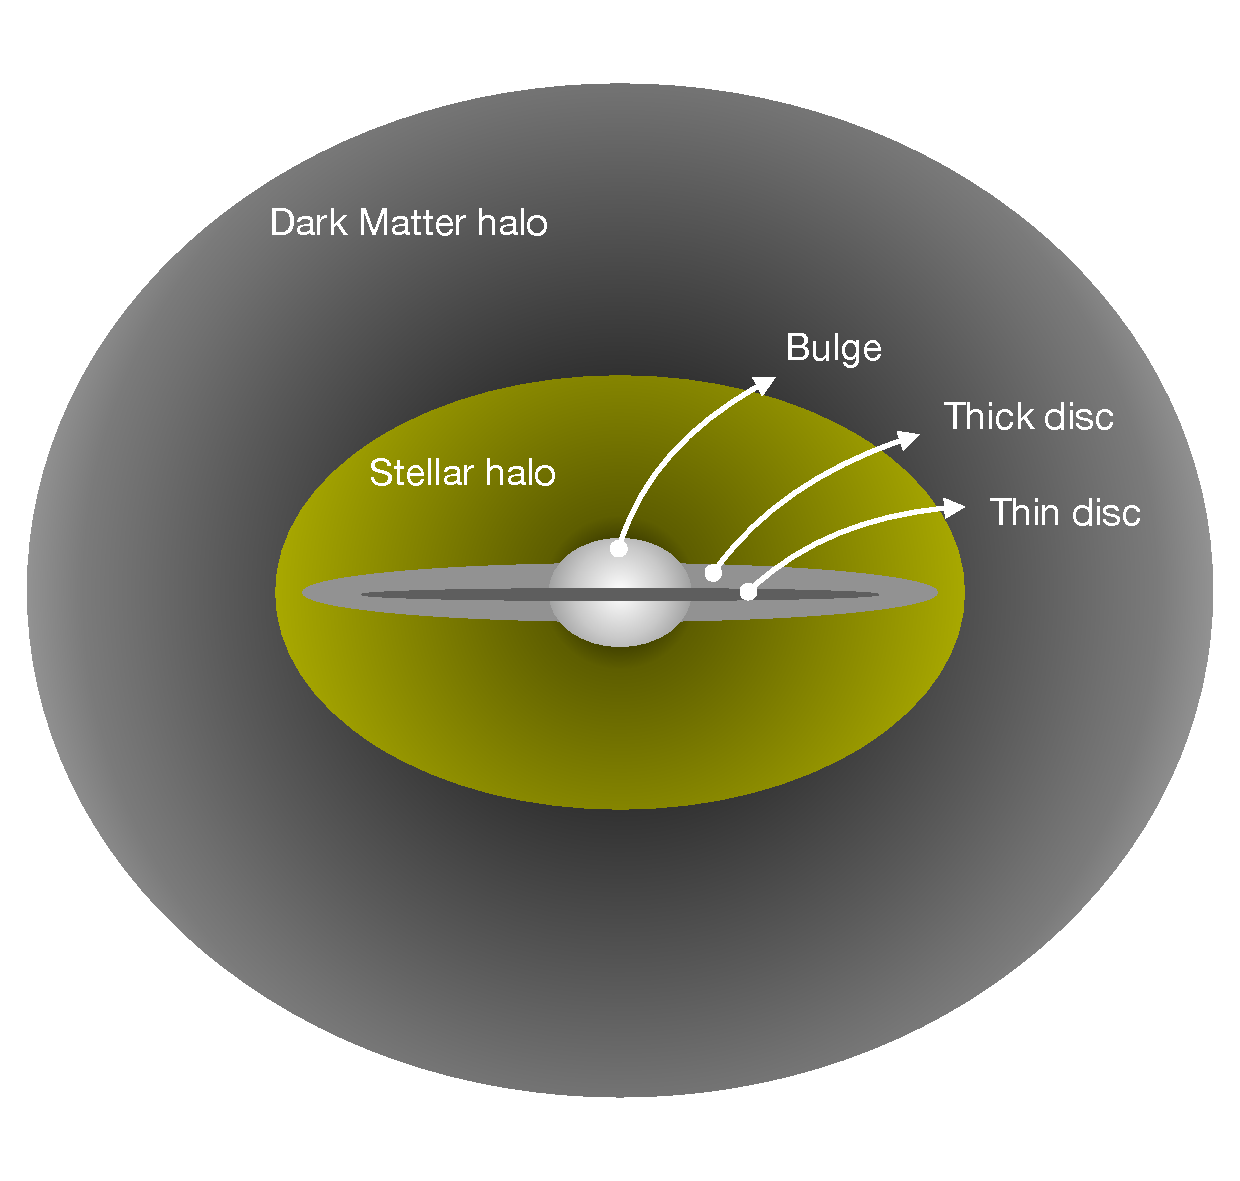
\includegraphics[width=0.95\columnwidth]{Kap1/diagram_disk_galaxy.pdf}
  \caption{ Diagram of the main components of disc-like galaxies: spheroidal bulge, thin and thick discs, spheroidal stellar and Dark Matter halos.}
  \label{fig:Fig_diagram_galaxy}
\end{figure}

El modelo dinámico de una galaxia obtenido de la curva de rotación es un estimativo a primera aproximación, dado que la velocidad circular es muy sensible a perturbaciones impuestas por ejemplo por brazos espirales, disco contra-rotante, movimientos disipativos del gas conocidos como\emph{inflows/outflows}, por lo que se requiere una descripción completa del modelo dinámico. La formulación de las ecuaciones de Jeans y del parámetro de anisotropía de las velocidades dan cuenta del elipsoide de velocidades que permite caracterizar con mayor exactitud el modelo y verificarlo respecto observables astrofísicos como la dispersión de velocidades y el campo de velocidades. La curva de rotación es especialmente precisa en modelar la dinámica a grandes distancias del centro galáctico, pero en la región central la forma de la curva de rotación carece de una definición clara.\\








\chapter{Dinámica estelar}

\section{Teoría del potencial}

Una galaxia es un sistema de estrellas, gas interestelar y materia oscura que interacciona entre ellos fundamentalmente siguiendo la teoría de gravedad de Newton. La masa total de una galaxia tipo disco está compuesta de diferentes masas asociadas con sus sistemas estelares constituyentes. Las distribuciones de masa darán la forma funcional para los potenciales de acuerdo a la ley de gravedad de Newton expresada en forma diferencial por la \textbf{ecuación de Poisson} \cite{Samurovic07, BT08}:
\begin{equation}
\label{PT2}
\nabla^2 \Phi (\textbf{x}) = 4\pi  G \rho (\textbf{x}).
\end{equation}

La \textbf{ecuación de Poisson} es una ecuación diferencial parcial que permite linealidad: si el potencial genera $\rho_1$, y $\Phi_1$, y $\rho_2$ genera $\Phi_2$, entonces la suma $\rho_1 + \rho_2$ genera la suma $\Phi_1+ \Phi_2$. Cuando se pueda hacer $\Phi(\textbf{x}\rightarrow \infty) = 0$ la solución a la ecuación (\ref{PT2}) es:
\begin{equation}
\label{PT1}
\Phi(\textbf{x}) = -G \int \textrm{d}^3   \textbf{x'} \frac{\rho(\textbf{x'})}{| \textbf{x'}-\textbf{x} |},
\end{equation}
donde $G$ es la constante de gravitación universal, y la integral es tomada sobre toda la distribución de masa.

Como se vio antes (\ref{PT2}) admite superposición de componentes de masa y permite encontrar el potencial total para la galaxia que es necesario para calcular por ejemplo la velocidad circular. 

\subsection{Par densidad - potencial gravitacional de galaxias tipo disco}

Es una tarea difícil resolver la ecuación de Poisson para $\Phi(\textbf{x})$ dada la densidad de masa $\rho (\textbf{x})$. Sin embargo, soportado por las consideraciones de simetría y los perfiles de luminosidad es posible simplificar el problema y encontrar una forma funcional para la distribución de masa de una galaxia espiral como en \cite{Miyamoto75}.

Como una primera aproximación a la dinámica real de galaxias tipo disco, su distribución de masa puede ser descompuesta principalmente en tres masas: bulbo (o \emph{bulge}), disco y el halo de materia oscura \cite{S16}. A continuación se presentan en contexto el desarrollo histórico de esos componentes, las formas funcionales para sus potenciales gravitacionales y su importancia en el entendimiento de la curva de rotación de galaxias tipo disco.

\subsubsection{Potencial de Miyamoto-Nagai}
Expresa las componentes de masa de un bulbo o cúmulo central de estrellas y un disco delgado/grueso de una galaxia. El potencial de Miyamoto - Nagai es una generalización de los potenciales de Plummer y Kuzmin.

En 1911, Plummer usó una solución elemental de la \textbf{ecuación de Lane-Emden} para encontrar el potencial gravitacional de un sistema esférico. La \textbf{ecuación de Lane-Emden} relaciona el radio adimensional $s=r/d$ con $\psi = \Psi/\Psi_0$, una cantidad involucrando la densidad $\rho$ \cite{BT}:

\begin{equation}
\label{Lane_Emden}
 \frac{1}{s^2} \frac{d}{ds} \left ( s^2 \frac{d \Psi}{ds} \right ) = \left\{
	\begin{array}{ll}
		-3\Psi^n  & \mbox{if } \psi > 0 \\
		0 & \mbox{if } \psi \leq 0
	\end{array}
\right.
\end{equation}
con
$d=(4/3 \pi G \Psi_0^{n-1}c_n)^{-1/2}$ y las condiciones de frontera $\psi(0) = 1, d\psi/ds|_0 = 0$; de una esfera de gas politropica, donde la presión $P$ es proporcional a una potencia de la densidad $\rho$ dada por el índice politropico $n$, 
 $$ P=K \rho^{1+1/n}. $$

Un sistema esférico auto-consistente conocido como el modelo de Plummer corresponde a una solución exacta de la \textbf{ecuación de Lane-Emden}, y sus condiciones de frontera con la polítropa $n=5$ de acuerdo a los resultados de Schuster en 1883 \cite{Miyamoto75, BT}:
$$\Phi_P (R,z) = - \frac{GM}{\sqrt{R^2+z^2+b^2} } = - \frac{GM}{\sqrt{r^2+b^2} }$$
con $r^2 = R^2+z^2 .$ El modelo de Plummer surgió de la discusión acerca de la distribución de estrellas en los cúmulos estelares. La densidad de masa a diferencias distancias del centro de los cúmulos estelares es aproximadamente el mismo, y se asume que esos sistemas vienen de distribuciones esféricas \cite{Plummer11}.\\

Adicionalmente, para una distribución de masa plana de galaxias axialmente simétrica, Toomre en 1963 encontró las soluciones exactas para la \textbf{ecuación de Poisson}
$$\nabla^2 \Phi (\textbf{x}) = 4\pi  G \mu(R) \delta(z),$$
donde $\mu(R)$ y $\delta(z) $ son la densidad superficial de masa y la función Delta de Dirac. La solución está dada por \cite{Miyamoto75, BT}:
$$\Phi_K (R,z) = - \frac{GM}{\sqrt{R^2+(a+|z|)^2} }$$
denominado el modelo de Kuzmin o modelo 1 de Toomre.\\

El potencial de Miyamoto - Nagai es un potencial definido en coordenadas cilíndricas $(R,z)$ por:

\begin{equation}
\label{MN1}
\Phi_{MN} (R,z) = - \frac{GM}{\sqrt{R^2+(a+\sqrt{z^2+b^2})^2}}
\end{equation}

donde $a$, $b$, $M$ son las escalas de altura  y masa encerrada en una distancia galactocéntrica  $R$, y estas pueden ser usadas como parámetros para determinar las componentes de masa. La figura  (\ref{fig:Fig_MN_parameters}) representa los cambios en la forma de la curva de rotación por tres valores de amplitud. Esos valores están trazados por la cantidad $GM$ (arriba) que representa la masa en el modelo de Miyamoto-Nagai y la escala de altura $b$ (abajo) que determina la planitud de la densidad de masa (mejor trazada por la razón de escala $b/a$). El modelo (\ref{MN1}) es libre de singularidades y tiende al potencial de masa puntual Newtoniano cuando $R$ y $z$ llegue a ser grande \cite{Miyamoto75}.\\

El potencial es una generalización de los potenciales de Plummer y Kuzmin
$\Phi_P (R,z)$ y $\Phi_K (R,z)$ respectivamente. Un potencial esféricamente  simétrico (esto es, un modelo Plummer) puede ser expresado usando los parámetros de escala definidos en el potencial de Miyamoto-Nagai (\ref{MN1}) con $a=0$ \cite{Samurovic}, y $b=0$ un modelo de Kuzmin. Para éste ultimo caso, la curva de rotación es mostrada en la figura (\ref{fig:Fig_MN_parameters}) (abajo) obteniendo menores valores de $b$ tal que la velocidad circular tiene un crecimiento inferior en la región central de pocos kpc.

El potencial de  Miyamoto-Nagai describe geometrías de bulbo y disco continuamente, incluyendo potenciales de Plummer y Kuzmin sin superponerlos \cite{Miyamoto75}. 
 
\begin{figure}
  \centering
    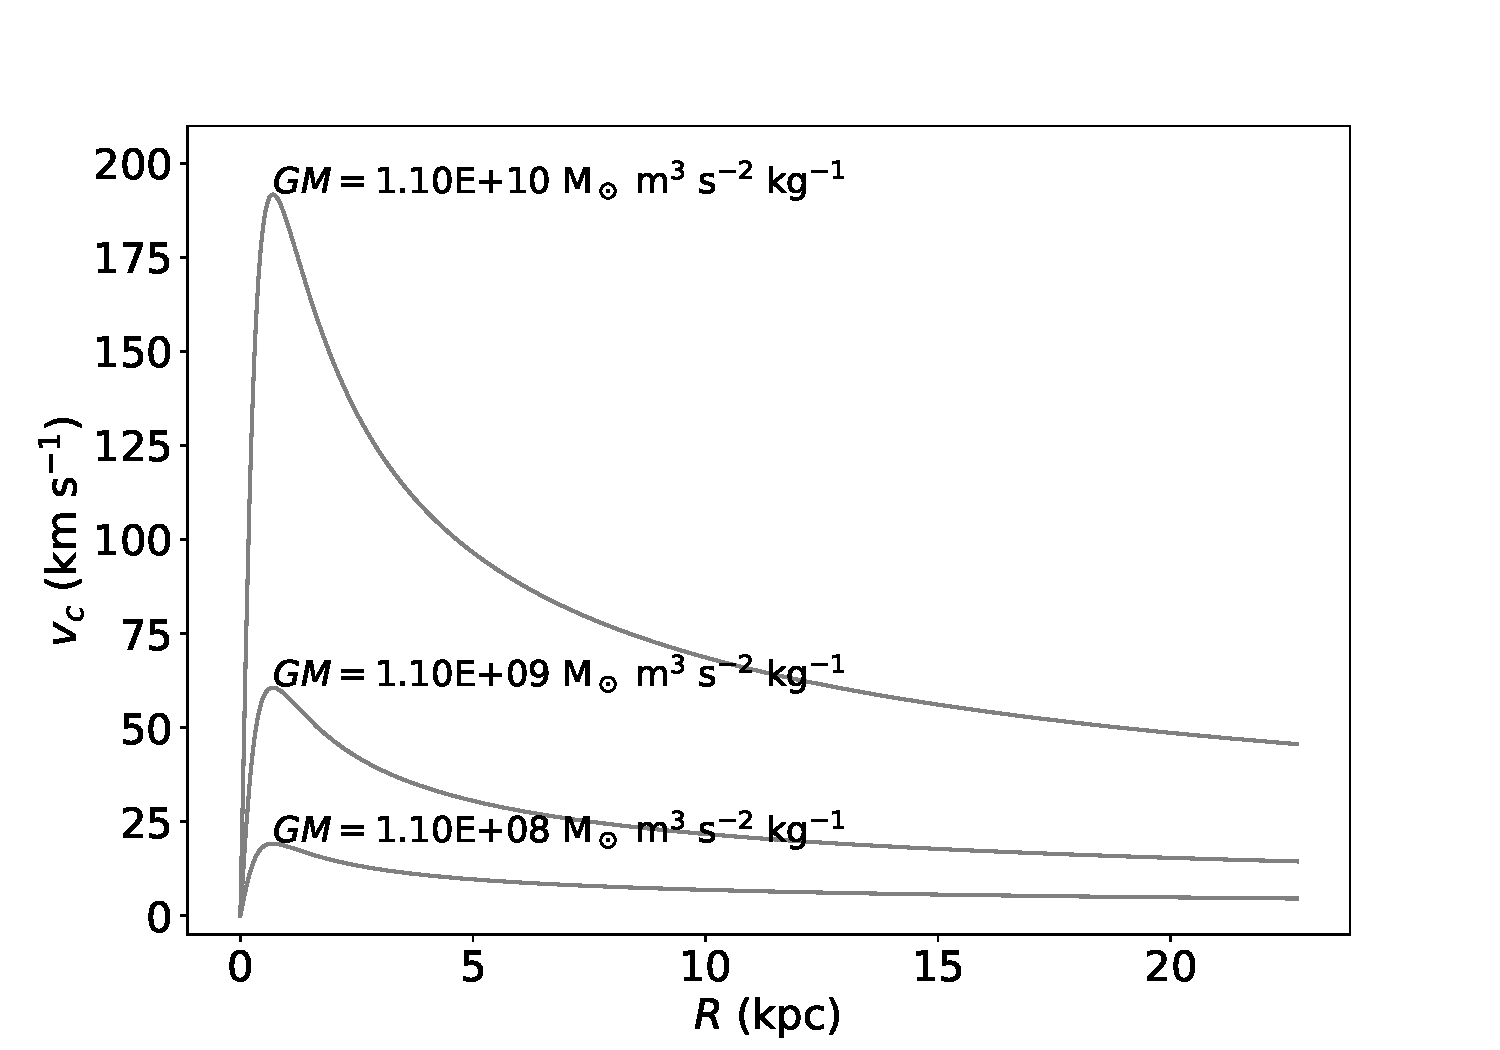
\includegraphics[width=0.8\columnwidth]{Kap2/MN_Amp.pdf}
    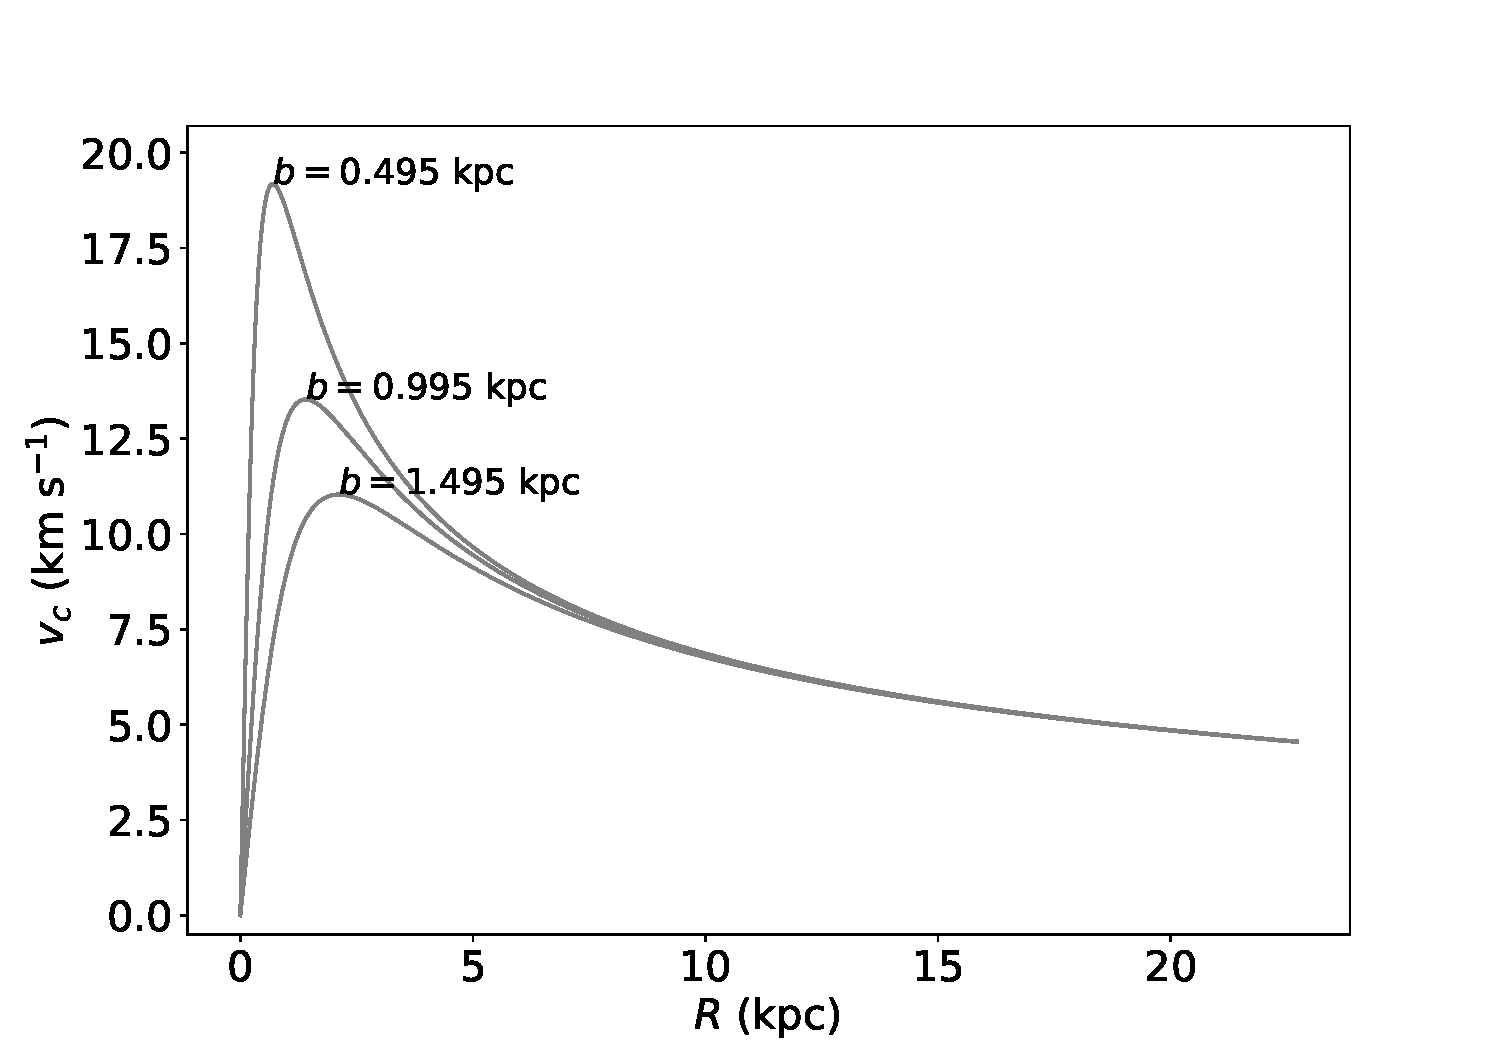
\includegraphics[width=0.8\columnwidth]{Kap2/MN_b.pdf}
  \caption{ Curva de rotación usando el potencial de Miyamoto-Nagai con tres valores de amplitud $GM$ (arriba) y del parámetro de escala $b$ (abajo).}
  \label{fig:Fig_MN_parameters}
\end{figure}


\subsubsection{Potencial de disco exponencial}
Un disco delgado axialmente simétrico puede ser considerado un esferoide muy plano. A continuación, se mostrará el potencial gravitacional de un esferoide  delgado infinitesimal asumiendo algunas condiciones físicas y geométricas.\\

El volúmen de un esferoide oblato de radios ecuatorial y polar son $a, c$ respectivamente es $V=4\pi a^2c/3$ y su densidad es $\rho$ entonces la masa total entre el radio $a$ es $M(a)=\frac{4}{3} \pi \rho q a^3$ asumiendo densidad constante.

De acuerdo a la figura (\ref{fig:Fig_Galaxy_Spheroid}), la distancia a lo largo del eje polar permite expresar la masa encerrada en un radio $R$, donde el eje polar está a lo largo de la dirección $z$, y el plano ecuatorial está en $x-y$. Así, el disco galáctico puede ser encontrado llevando la altura de la distribución de masa $z$ hacia el plano ecuatorial.

\begin{figure}
\centering%
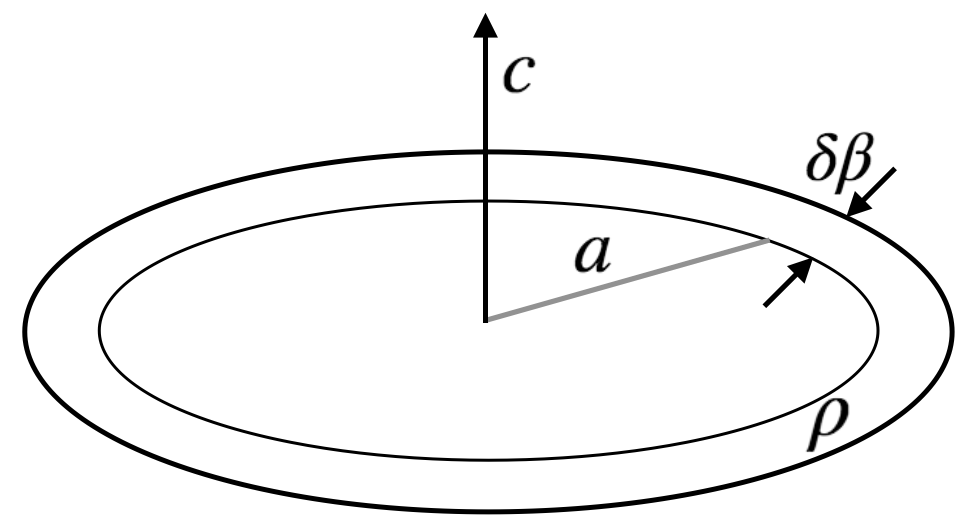
\includegraphics[width=0.45\columnwidth]{Kap2/homoeoid2D.png}
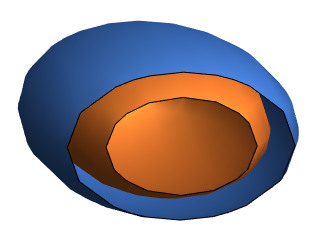
\includegraphics[width=0.45\columnwidth]{Kap2/homoeoid3D.png}
\caption{Homoeoide 2D con densidad $\rho$ y grosor $\delta\beta$ (izquierda) y 3D (derecha) }
\label{fig:homoeoid}
\end{figure}


La relación geométrica del esferoide es

$$ \frac{x^2}{a^2} + \frac{y^2}{a^2} + \frac{z^2}{c^2} = \frac{R^2}{a^2} + \frac{z^2}{c^2} = 1, $$

con $q=c/a$, la distancia polar $ z = q\sqrt{a^2 - R^2} $. Por lo tanto la densidad superficial es $\Sigma (a,R) = \rho z = 2\rho q \sqrt{a^2-R^2}$.

Entonces, calculando la masa y el diferencial de la densidad superficial por un cambio en la  distancia $a$, se obtienen las siguientes cantidades del homoeoide plano:

$$ \delta M(a) = 2\pi \Sigma_0 a \delta a \hspace{ 2cm } \delta \Sigma(a,R) = \frac{\Sigma_0 \delta a}{\sqrt{a^2-R^2}}, $$

con densidad central $\Sigma_0 = 2\rho q a$ a un radio fijo $a$. Ahora dejando el radio galactocentrico $R$ como un parámetro para la densidad superficial $\Sigma_0(a)$ dependiendo solo de $a$, que satisface \cite{BT}:

\begin{equation}
\label{ED4_5}
\Sigma (R) = \int_R^\infty da \frac{\Sigma_0(a)}{\sqrt{a^2-R^2}}, \end{equation}

con  $\Sigma(R)$ un modelo arbitrario de densidad superficial observado. La ecuación (\ref{ED4_5}) tiene una solución dada por la \textbf{ecuación integral de Abel}:

\begin{equation}
\label{ED5}
\Sigma_0(a) = -\frac{2}{\pi} \frac{d}{da} \int_a^{\infty} dR \frac{R\Sigma (R)}{\sqrt{R^2-a^2}}.
\end{equation}

\begin{figure}
  \centering
    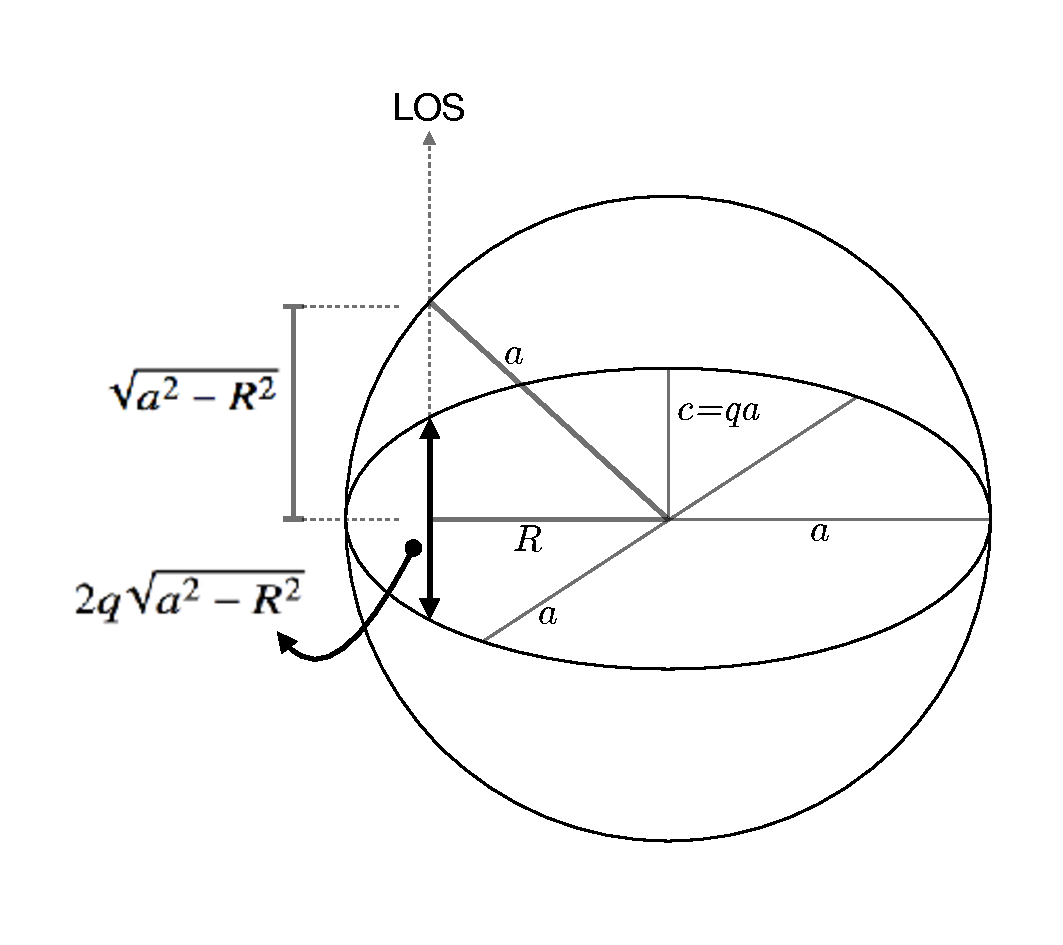
\includegraphics[width=0.95\columnwidth]{Kap2/galaxy_spheroid.pdf}
  \caption{ Esferoide de razón axial $q=c/a$. La línea de visión o (\emph{Line Of Sight - LOS}) es perpendicular al plano ecuatorial y cruza una distancia $2q\sqrt{a^2-R^2}$ a un radio galactocentrico radius $R$ del centro.}
  \label{fig:Fig_Galaxy_Spheroid}
\end{figure}

Ahora, siguiendo el método de separar la \textbf{ecuación de Laplace} en coordenadas cilíndricas y usando el Teorema de Gauss para obtener un par $\Sigma, \Phi$ como está detallado en \cite{C93} el Anexo A:

\begin{eqnarray*}
\Sigma_k (R) &=& \frac{k}{2\pi} J_0 (kR) \\
\Phi_k (R,z) &=& -G J_0(kR) exp(-k|z| ),
\end{eqnarray*}

donde $J_0$ es una función de Bessel cilíndrica; el potencial de disco resultante es una superposición de los componentes anteriores

$$ \Phi (R,z) = -2\pi G \int_0^{\infty} \int_0^{\infty} \Sigma(R') J_0(kR') R' J_0 (kR) exp(-|z|k) dR' dk. $$

Usando las propiedades en la forma integral de la función de Bessel $J_0$, puede ser construido un potencial de disco muy delgado como un homoeoide aplanado infinitesimal:

$$\delta\Phi= -2{\pi}G\Sigma_0\delta a{sin^{-1}} \left (\frac{2a}{\sqrt{z^2+(a+R)^2}+{\sqrt{z^2+(a-R)^2}}} \right ), $$

entonces el potencial para discos con simetría axial con densidad superficial $\Sigma(R)$, descompuesto en homoeoides usando las ecuaciones (\ref{ED4_5}, \ref{ED5}) puede ser expresado por:

$$ \Phi(R,z) = 4G \int_0^{\infty} \textrm{d}a sin^{-1} \left ( \frac{2a}{\sqrt{+}+\sqrt{-}} \right ) \frac{d}{da} \int_a^{\infty} dR' \frac{R'\Sigma (R')}{\sqrt{R'^2 - a^2}}$$

con una notación conveniente $\sqrt{\pm} = \sqrt{z^2+(a^2\pm R^2)^2}.$

Finalmente, integrando en $a$, el potencial para un disco axialmente simétrico en el plano (cuando $z \rightarrow 0$) es:

\begin{equation}
\label{ED2}
\Phi(R,0) = -4G \int_0^{\infty} \frac{da}{\sqrt{R^2-a^2}} \frac{d}{da} \int_a^{\infty} dR' \frac{R'\Sigma (R')}{\sqrt{R'^2 - a^2}}.
\end{equation}

De acuerdo con \cite{Freeman}, puede ser asumido que la razón masa-luminosidad es aproximadamente uniforme, como mínimo sobre el disco de una galaxia y entonces el perfil de densidad superficial está dado por la forma:

\begin{equation}
\label{ED1}
\Sigma_d (R) = \Sigma_{dc} exp(-R/R_d)
\end{equation}

conocido como el \textbf{disco exponencial}, donde $\Sigma_{dc}$ y $R_d$ son la densidad de masa superficial central y la escala radial respectivamente. La figura (\ref{fig:Fig_ED_parameters}) muestra el cambio en la forma de la curva de rotación por un cambio en los parámetros de potencial de la ecuación (\ref{ED1}). Un cambio en $\Sigma_{dc}$  representa desde una velocidad circular muy plana hasta un disco grueso (figura \ref{fig:Fig_ED_parameters} arriba), y valores pequeños en la escala de altura $h_r$ permite reproducir un disco plano.\\

Remplazar la densidad (\ref{ED1}) en la segunda integral de la ecuación (\ref{ED2}), es obtenido:

$$\int_a^{\infty} dR' \frac{R' \Sigma_0 e^{-R'/R_d}}{\sqrt{R'^2 - a^2} } = \Sigma_0 a K_1 (a/R_d)$$
adicionalmente, el potencial en el plano ecuatorial en términos de las funciones de Bessel modificadas $K_0, K_1$ y $I_0, I_1$, toma la forma:

\begin{equation}
\label{ED3}
\Phi_{ED}(R,z) = -\pi G\Sigma_0 R \left ( I_0(y)K_1(y) - I_1(y)K_0(y) \right )
\end{equation}

donde $y=R/2R_d$. Para una mayor discusión mirar \cite{Freeman, BT, C93}.

Para este modelo la masa total del disco está dada por \cite{Freeman}:
\begin{equation}
\label{massdisc}
M_d = 2\pi a^2 \Sigma_{dc},
\end{equation}

que depende sólo sobre los dos parámetros libres, la escala de radio $a$ y la densidad superficial central $\Sigma_{dc}$.\\

\begin{figure}
  \centering
    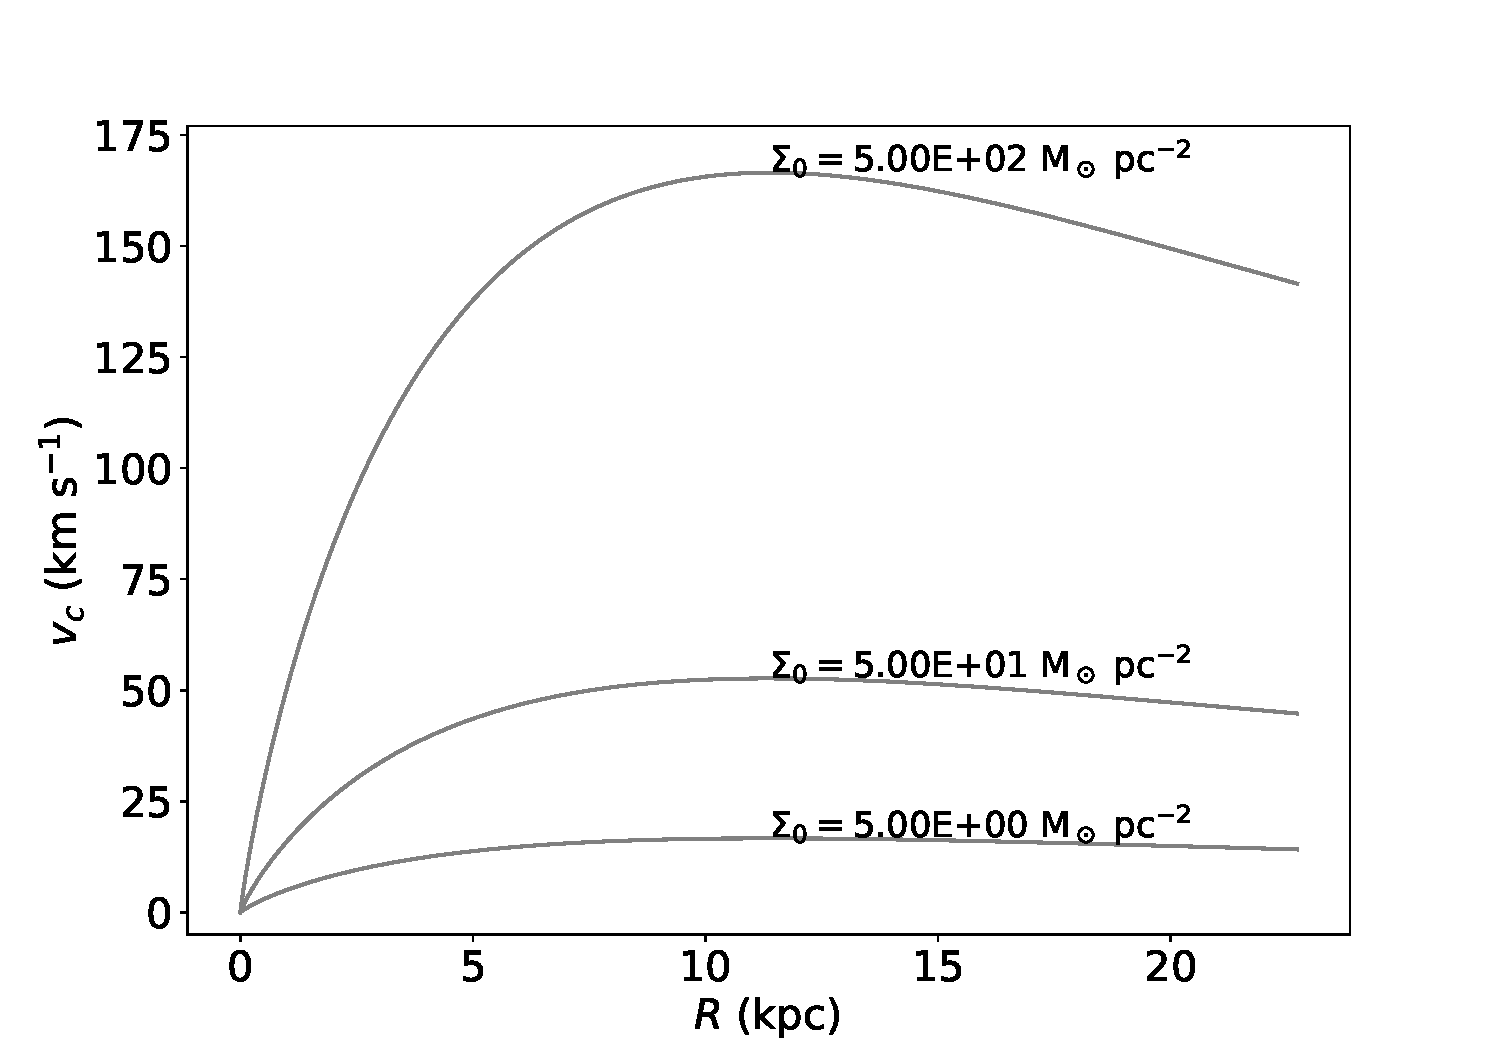
\includegraphics[width=0.8\columnwidth]{Kap2/ED_Amp.pdf}
    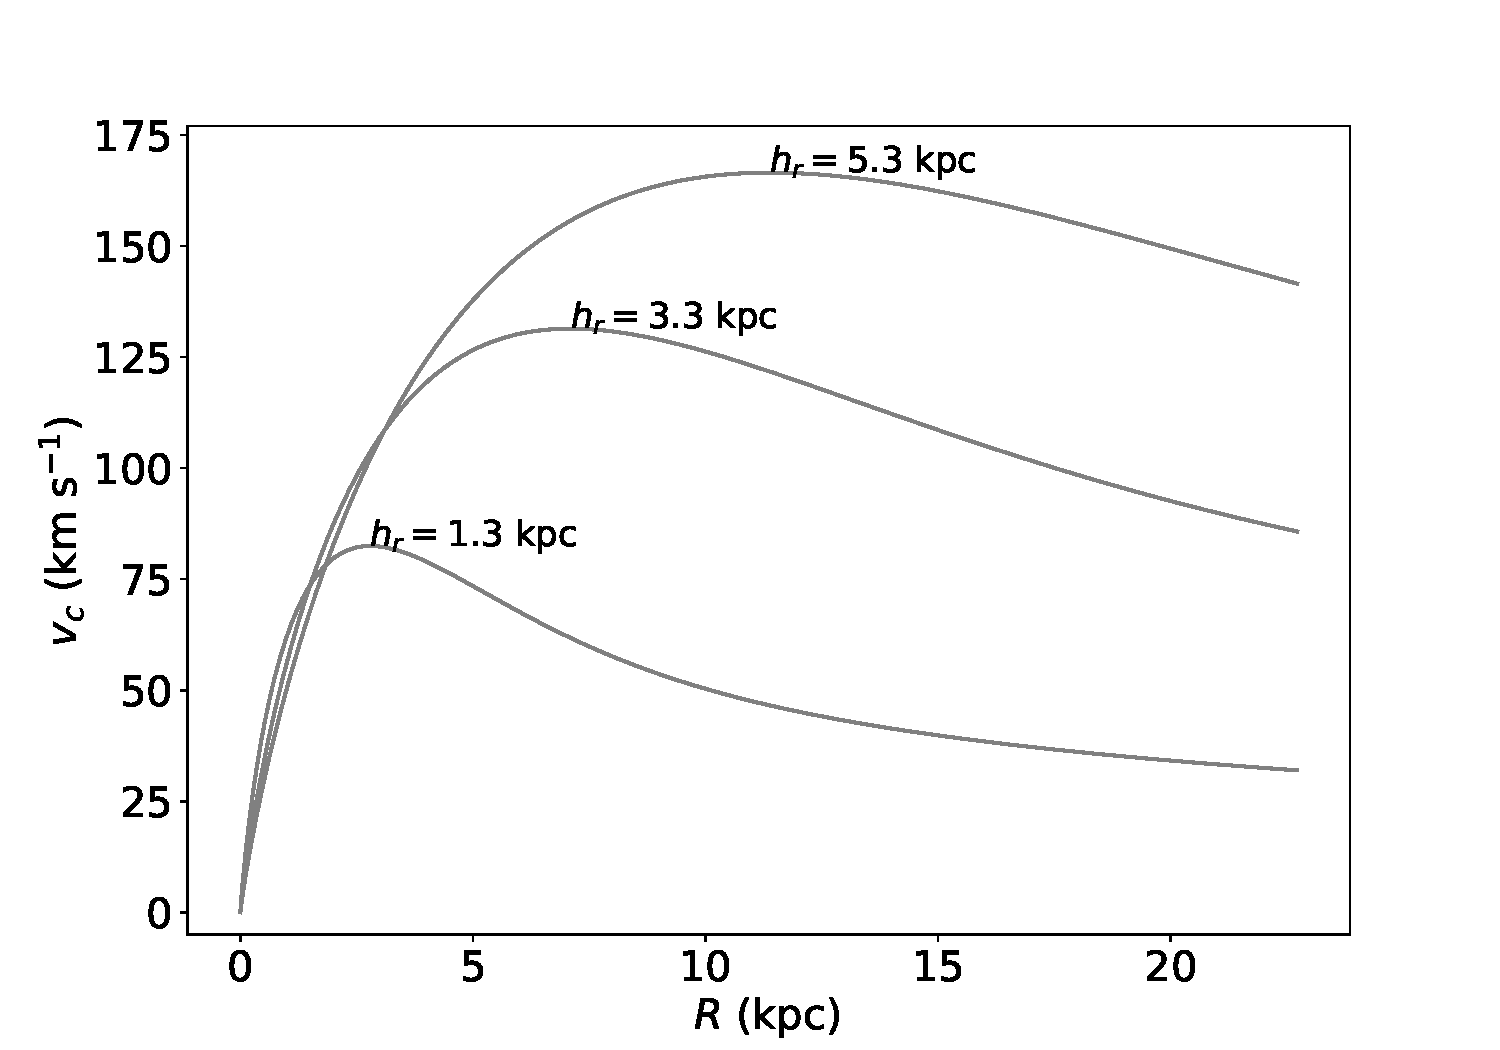
\includegraphics[width=0.8\columnwidth]{Kap2/ED_hr.pdf}
  \caption{ Curva de rotación usando un potencial de disco exponencial con tres valores de la densidad superficial $\Sigma_0$ (arriba) y la escala de parámetro $h_r$ (abajo).}
  \label{fig:Fig_ED_parameters}
\end{figure}

Un método complementario para encontrar el potencial del disco exponencial está dado por la definición de la luminosidad por unidad de área o brillo superficial de la galaxia \cite{BT}:

$$ I = \int_0^{\infty} dr j(\textbf{r}) $$
con $ j(\textbf{r}) $ la distribución de luminosidad. Dado la notación de la figura (\ref{fig:Fig_Galaxy_Spheroid}) en coordenadas cilíndricas la proyección de un cuerpo esférico donde $ a=r $ y la línea de visión (LOS) está a lo largo de la coordenada  $z$, resulta en el brillo superficial:

$$ I(R) = 2\int_0^{\infty} dz j(\textbf{r}) $$

y con la restricción geométrica  $ r^2 = R^2 + z^2 $ entonces $ r = \sqrt{r^2-R^2} $ y por lo tanto $dz = r dr / z$. La ecuación anterior resulta en 

$$ I(R) = 2 \int_R^{\infty} \frac{j(\textbf{r}) r dr}{\sqrt{r^2 - R^2}}, $$

que puede ser invertida en forma directa usando la identidad integral de Abel:

$$ j(\textbf{r}) = -\frac{1}{\pi} \int_r^{\infty} \frac{dI}{dR} \frac{dR}{\sqrt{R^2-r^2}}. $$

Bajo la suposición que algunos valores de la razón masa-luminosidad, la densidad volumetrica de masa $\rho(r)$ es proporcional a la densidad de brillo $j(\textbf{r}) $ por:

$$ \rho(r) = \frac{M}{L} j(\textbf{r}). $$

Entonces, de la densidad bidimensional $I(R)$ puede ser encontrada la densidad de luminosidad en el espacio $ j(\textbf{r}) $ y si la luz traza el desplazamiento de la masa, puede ser derivado la densidad de masa del sistema\\

\subsubsection{Potencial de Navarro-Frenk-White}

Las simulaciones de N cuerpos sin colisiones del agrupamiento de partículas de materia oscura sugiere que la densidad de masa entre un halo de materia oscura tiene una estructura similar a un modelo de ley de potencias de la densidad y un comportamiento de escala universal. Es interesante ver la similitud entre el perfil de luminosidad en galaxias elípticas  \cite{BT} y la distribución de masa en el halo de materia oscura. La densidad de masa está dada por una ley de potencias doble:

\begin{equation}
\rho (r) = \frac{\rho_0}{(r/a)^\alpha (1+r/a)^{\beta-\alpha}}.
\end{equation}

En particular $(\alpha, \beta) = (1,3)$ es llamada el modelo Navarro-Frenk-White (NFW) \cite{NFW}. Este modelo tiene dos parámetros libres: la escala de radio $a$ y la densidad representativa $\rho_0$. Este modelo tiene también dos parámetros correlacionados: la masa del halo $M_a(R)$  y su densidad característica  (adimensional) $\delta_0$ \cite{NFW}. Finalmente la densidad del modelo NFW es:

$$\rho (r) =  \frac{\rho_0}{(r/a) (1+r/a)^2} = \rho_c \frac{\delta_0}{(r/a) (1+r/a)^2},$$

donde $\rho_c = 3H_0^2/8\pi G $ es la densidad crítica del halo. El potencial es:

\begin{equation}
\label{NFW0}
\Phi_{NFW} (r) = -4\pi G \rho_0 a^2 \frac{ln (1+r/a)}{r/a}.
\end{equation}

La masa encerrada entre un radio $R$ es (de \cite{J03}):

\begin{equation}
M_a(R) = 4\pi \rho_0 a^3 \left[  \textrm{ln} \left (  1+\frac{R}{a} \right ) - \frac{R/a}{1+R/a} \right ]
\label{eq:NFW_M}
\end{equation}

Alternativamente,  simulaciones numéricas y la teoría del colapso gravitacional en el universo cercano mostraron la importancia de definir la cantidad llamada el parámetro de concentración adimensional definido como \cite{Bosch}:
\begin{equation}
\label{NFW1}
X_{200}=r_{200}/a
\end{equation}
 donde: 
\begin{equation}
\label{NFW2}
M_{200}=200\rho_c \frac{4\pi}{3} r_{200}^3
\end{equation} 
es la masa crítica del halo de materia oscura, y  $r_{200}$ es la distancia crítica del centro del halo,  en el cual la densidad media es 200 veces la densidad crítica cosmológica $\rho_c$.

Usando el conjunto de ecuaciones anterior, puede ser encontrada la relación :

\begin{equation}
\label{NFW3}
  \textrm{ln}  (  1+X_{200} ) - \frac{X_{200}}{1+X_{200}} = \frac{200 \rho_c}{3\rho_0} X_{200}^2 \textrm{   ,}
  \end{equation}

y resolviendo la ecuación (\ref{NFW3}) para $X_{200}$ por aproximación sucesiva \cite{S16}, los parámetros $M_{200}, R_{200}$ pueden ser obtenidos de $\rho_0$ y $a$ ajustando la componente de masa del halo en la curva de rotación. Como puede ser visto en la figura (\ref{fig:Fig_NFW_parameters}), un incremento de la cantidad $GM$ resulta en mayor amplitud y cualquier cambio en el parámetro de escala $a$ da un crecimiento mas rápido (o mayor cobertura) en distancia galactocentrica de la galaxia.

\begin{figure}
  \centering
    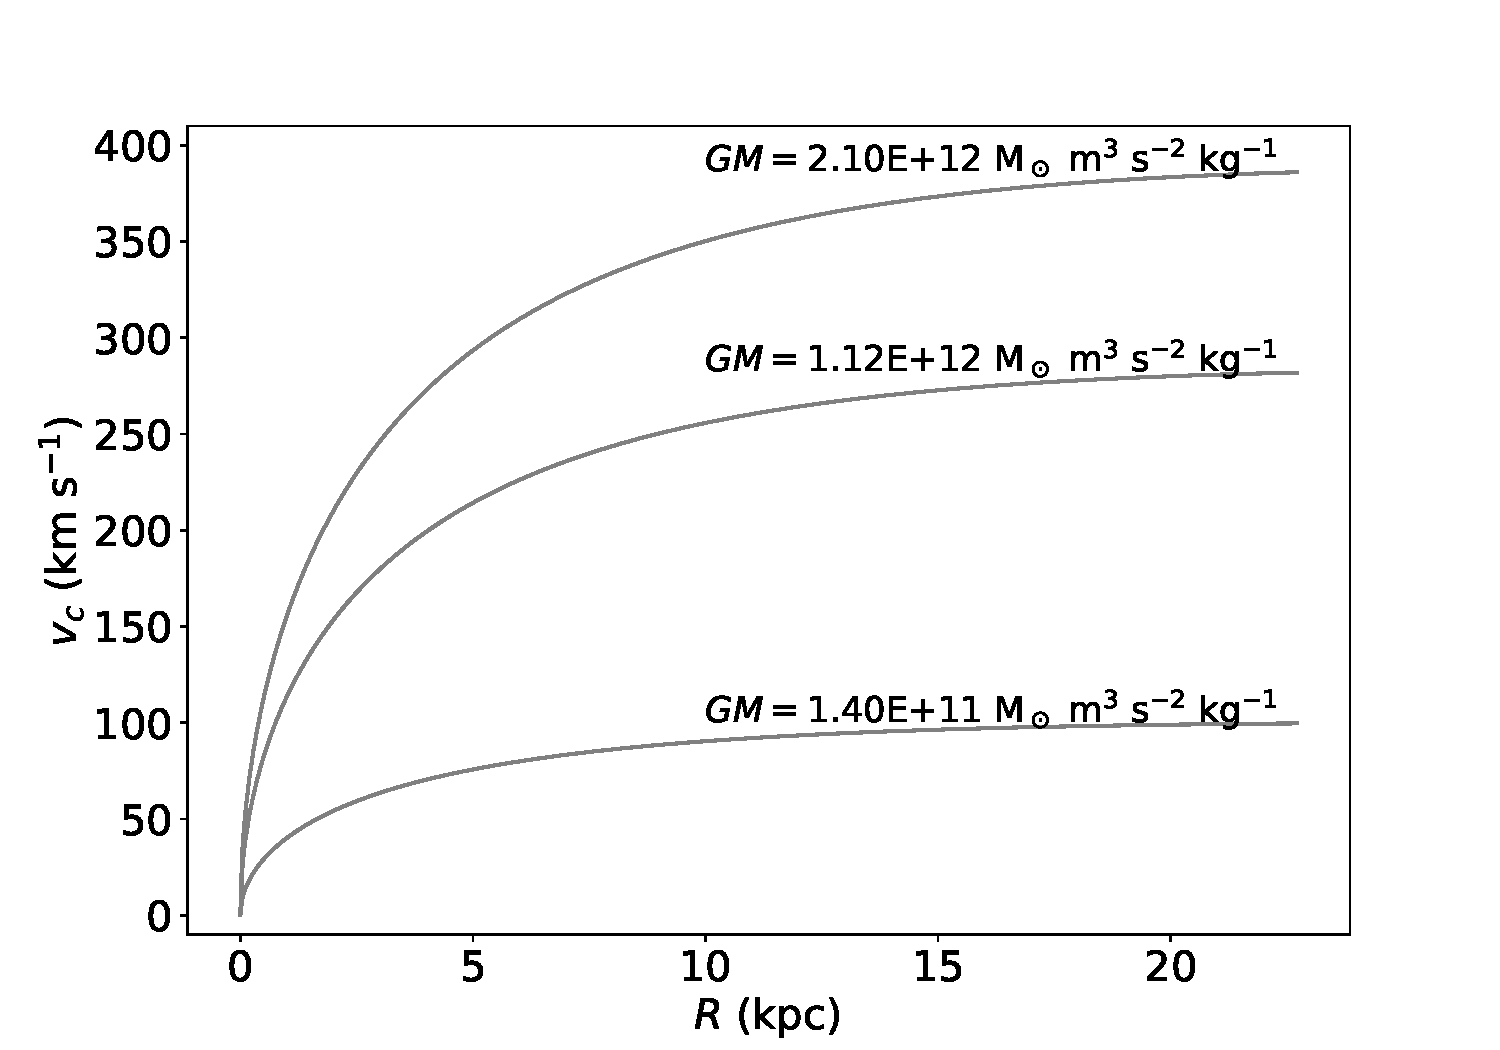
\includegraphics[width=0.8\columnwidth]{Kap2/NFW_Amp.pdf}
    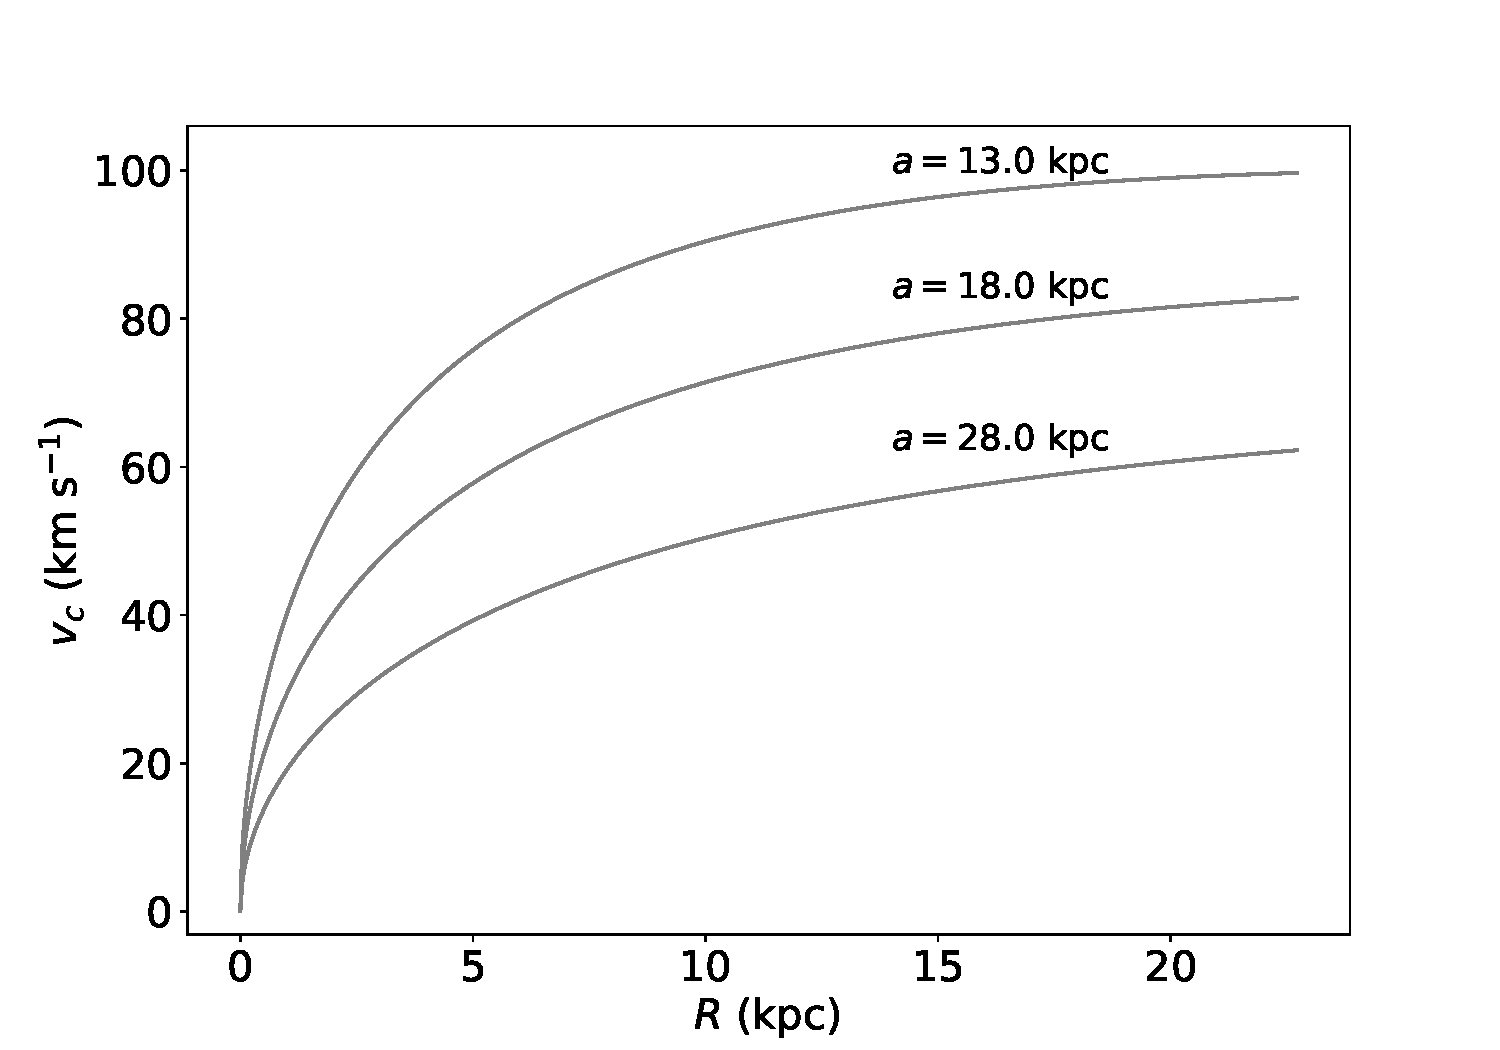
\includegraphics[width=0.8\columnwidth]{Kap2/NFW_a.pdf}
  \caption{ Curva de rotación usando un potencial de Navarro-Frenk-White con tres valores de la amplitud $GM$ (arriba) y el parámetro de escala del radio $a$ (abajo).}
  \label{fig:Fig_NFW_parameters}
\end{figure}

\subsubsection{Potencial de Burkert}

Algunas galaxias enanas  están completamente dominadas por Materia Oscura y los perfiles de densidad están de acuerdo a la densidad en el centro dado por la ley isoterma (\ref{isothermal}). Esta ley satisface el valor constante  en la parte exterior de la curva de rotación porque decae proporcionalmente como $r^{-2}$ \cite{Burkert95}:

\begin{equation}
\label{isothermal}
\rho(r) =	\frac{\rho_0}{1+r^2/r_c^2},
\end{equation}
donde $r_c$ es el radio del núcleo y  $\rho_0$ es la densidad central de materia oscura.\\

Sin embargo, en simulaciones cosmológicas, el escenario de Materia Oscura Fría o (CDM - \emph{Cold Dark Matter} por sus siglas en inglés) predice halos con cúspide de densidad central que no han sido observadas para muchas galaxias enanas, espirales y galaxias de bajo brillo y masa \cite{L17}. Los perfiles de masa observados en galaxias enanas puede ser ajustado por la distribución de densidad fenomenológica de acuerdo a \cite{Burkert95}, conocido como el perfil de densidad de Burkert, dado por:

\begin{equation}
\label{Burkert_profile}
\rho_{BK}(r) = \frac{\rho_c r_c^{3}}{(r+r_c)(r^2+r_c^2)}
\end{equation}

con $\rho_c$ y $r_c$ parámetros que representan la densidad central del núcleo y una escala de radio. Esos valores no son independientes, el perfil de Burkert constituye una familia de un parámetro \cite{S00} usando las relaciones de escala para Materia Oscura en  \cite{Burkert95}:

\begin{eqnarray*}
\nu_0 &=& 17.7 (r_0 \textrm{kpc}^{-1})^{2/3} \textrm{kpc}^{-1}  \\
M_0 &=& 7.2 \times 10^{7} (r_0 \textrm{kpc}^{-1})^{7/3} \textrm{ M}_{\odot}\\
\rho_{0} &=& 4.5 \times 10^{-2} (r_0 \textrm{kpc}^{-1})^{-2/3} \textrm{ M}_{\odot} \textrm{pc}^{-3} \\
\end{eqnarray*}

Una propiedad interesante del perfil de Burkert está dado por la ley isoterma (\ref{isothermal}). Ésta puede ser reproducida con $(r<<r_0)$ en (\ref{Burkert_profile}) y la curva de rotación exterior constante diverge logaritmicamente. La correspondiente curva de rotación es mostrada en la figura \ref{fig:Fig_BK_parameters} cuando un cambio en la densidad del centro $\rho$ (arriba) da un valor específico en la amplitud del perfil de núcleo y un valor pequeño para la escala de radio $r_c$ (abajo)  resulta en una velocidad inferior para la misma pendiente central.

\begin{figure}
  \centering
    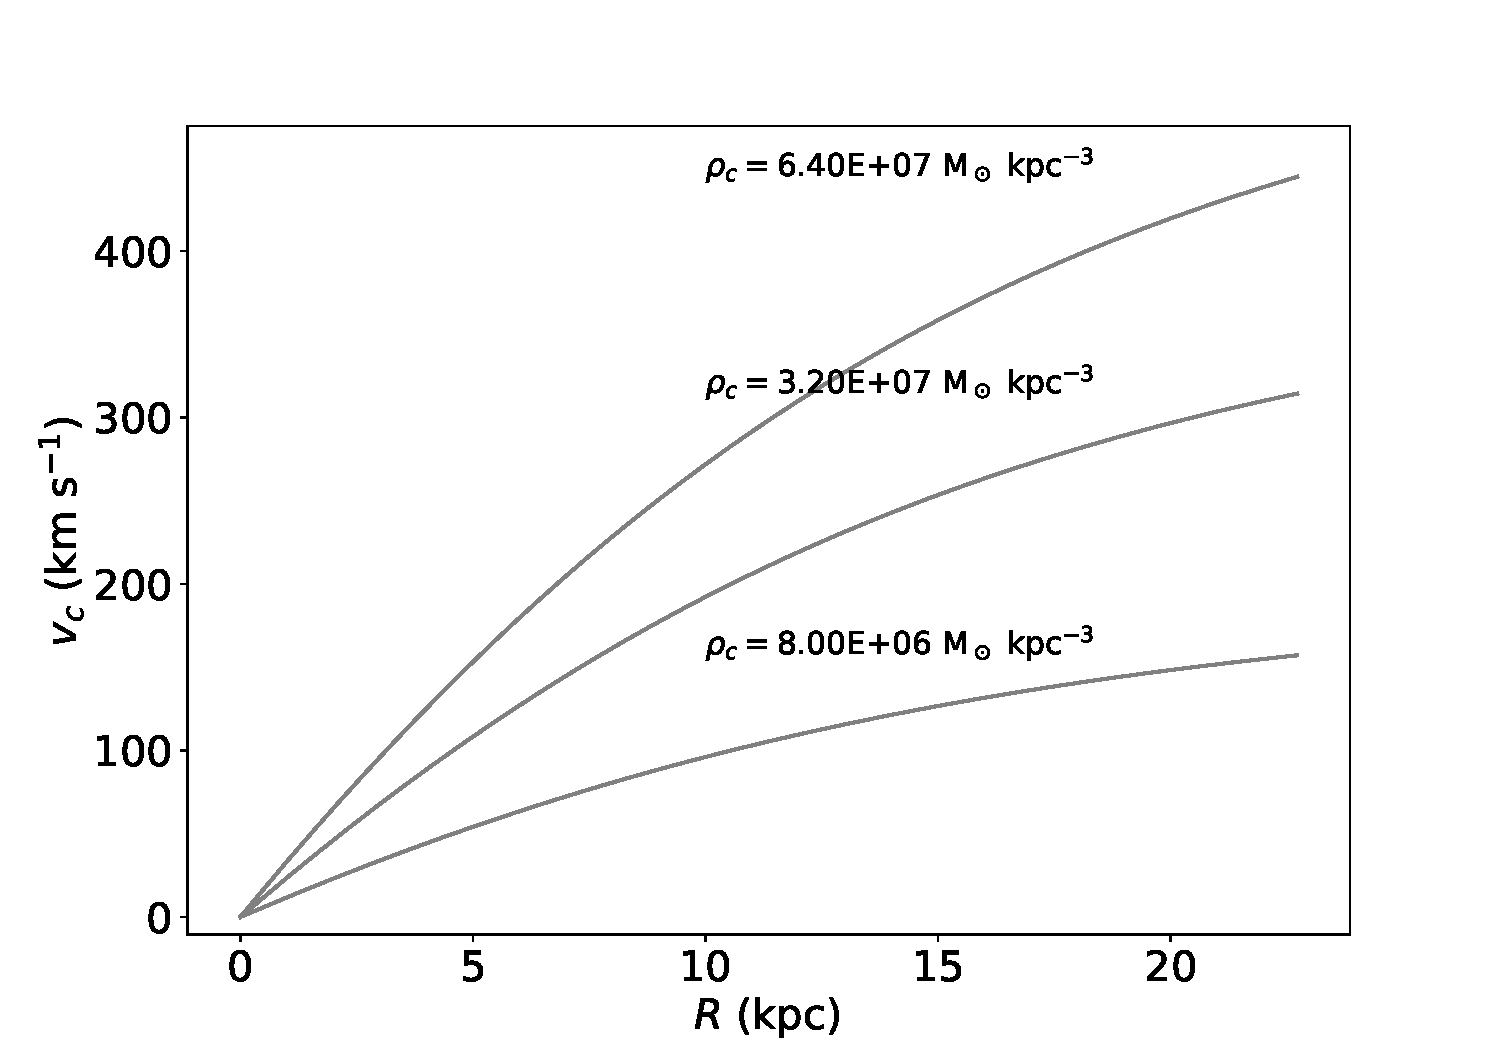
\includegraphics[width=0.8\columnwidth]{Kap2/BK_Amp.pdf}
    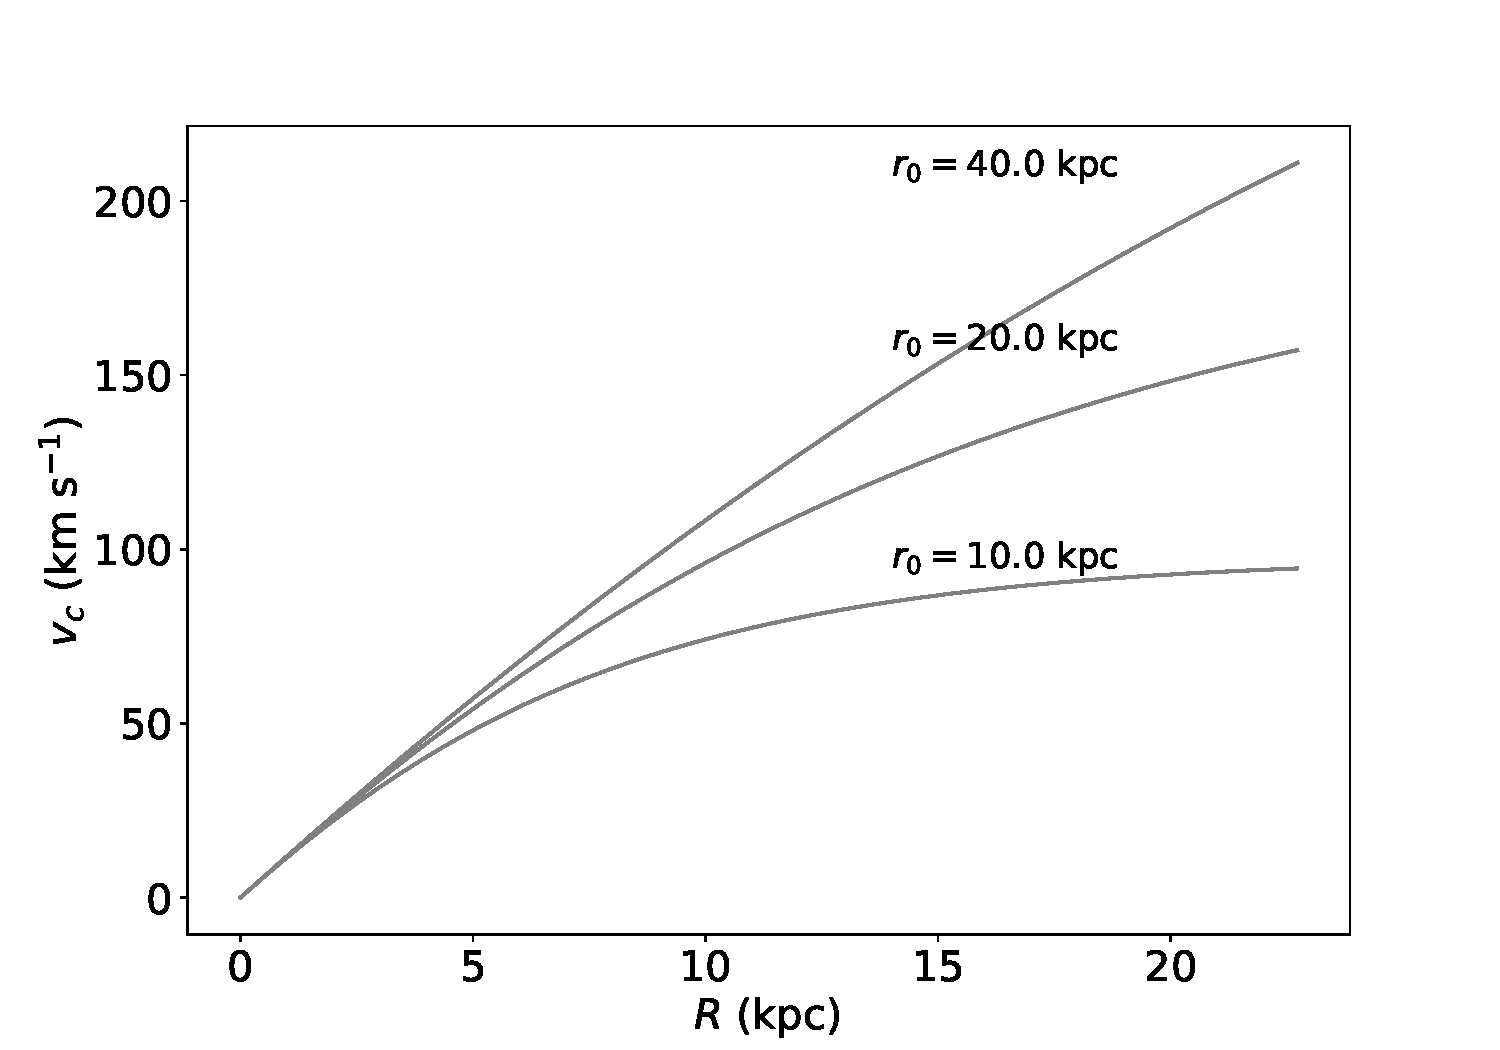
\includegraphics[width=0.8\columnwidth]{Kap2/BK_r.pdf}
  \caption{ Curva de rotación usando un potencial de Burkert con tres valores para la densidad central del núcleo $\rho$ (arriba) y el parámetro de escala radial $r_c$ (abajo).}
  \label{fig:Fig_BK_parameters}
\end{figure}

\subsection{Velocidad circular}

La velocidad $v_c$ a la que una estrella mantiene una órbita circular de radio $R$ con centro en el centro de la galaxia de potencial gravitacional $\Phi$, y asumiendo que el potencial es simétrico en torno al centro, es denominado \textbf{velocidad circular} y está relacionada con la aceleración radial del cuerpo $a_r$ por:

$$ a_r = \frac{\partial \Phi }{\partial R} = \frac{v_c^2}{R}, $$

esto es, la velocidad está descrita por el potencial de la forma:

\begin{equation}
\label{CV1}
v_{c}^2 = \frac{\partial \Phi}{\partial R} R.
\end{equation}

De acuerdo a la linearidad de la \textbf{ecuación de Poisson} (\ref{PT2}), si el sistema está compuesto por $n$ distribuciones de masa, el potencial gravitacional de todo el sistema está dado por:

\begin{equation}
\label{CV2}
 \Phi = \Phi_T = \sum_i^n \Phi_i.
\end{equation}

Entonces, de acuerdo a la ecuación (\ref{CV1}) y  a la composición de potenciales (\ref{CV2}), la velocidad circular total es:

\begin{equation}
\label{CV3}
v_{c}^2 = \sum_i^n v_i^2.
\end{equation}

Usando la ecuación (\ref{CV1}), fueron deducidos las velocidades circulares de los tres potenciales de las ecuaciones (\ref{MN1}, \ref{ED3}, \ref{NFW0}) respectivamente \cite{BT}:

\subsubsection{Potencial de Miyamoto-Nagai}
\begin{equation}
v_M (R) = R \sqrt{ \frac{GM}{ (R^2+(a+\sqrt{z^2+b^2})^2)^{3/2}}  }
\end{equation}

\subsubsection{Potencial disco exponencial}
\begin{equation}
v_{ED} = \sqrt{ 4\pi G \Sigma_0 R_d y^2 (I_0(y)K_0(y) - I_1(y)K_1(y)) }
\end{equation}

\subsubsection{Potencial de Burkert}
\begin{equation}
v_{BK} = \sqrt{ \frac{4GM_0}{r}  \left [ ln \left (1+\frac{r}{r_0} \right ) - tg^{-1} \left (\frac{r}{r_0} \right ) +\frac{1}{2} ln \left ( 1+\left (\frac{r}{r_0} \right )^2\right ) \right ] }
\end{equation}

where $M_0$ is the mass within the core.

\subsubsection{Potencial de Navarro-Frenk-White \cite{B15}}
\begin{equation}
v_{NFW} (R, z) = R \sqrt{   \frac{4\pi G a^2 \rho_0}{r^2(r+a)} - 4\pi G a^3 \rho_0\frac{log(r/a)+1}{r^{3/2}}  } 
\end{equation}

\section{Función de distribución}

La probabilidad de encontrar una estrella en el volumen del espacio de seis dimensiones dado por $d^3\textbf{x} d^3\textbf{v}$, con posición y velocidad dados $\textbf{x}, \textbf{v}$ respectivamente puede se calculada a partir de la función de distribución.

La función de distribución  $f (\textbf{x} ,\textbf{v}, t)$ cumple que su integral en un rango del espacio de fase es la probabilidad de encontrar una estrella escogida aleatoriamente en el tiempo $t$ es igual a la unidad, dado que se asumen partículas  idénticas:

$$ \int d^3\textbf{x} d^3\textbf{v} f (\textbf{x} ,\textbf{v}, t)  = 1 $$

Esta probabilidad es la misma si se calcula la integral del espacio de fase sobre cualquier sistema canónico coordenado $ \textbf{w} = (\textbf{q}, \textbf{p})$.

Se puede definir una probabilidad por unidad de volumen en una posición dada $\nu( \textbf{x} ) $, marginalizando la función de distribución respecto las velocidades:

\begin{equation}
\label{Dens_prob}
\nu( \textbf{x} ) \equiv \int d^3\textbf{v} f(\textbf{x}, \textbf{v}).
\end{equation}


Ésto permite encontrar una cantidad que se puede comparar con observables astrofísicos, como la densidad por unidad de volumen de número de estrellas del espacio real (o directo) $n ( \textbf{x} ) $ mediante como el producto del número de estrellas por la probabilidad por unidad de volumen:

$$ n ( \textbf{x} ) \equiv N \nu(\textbf{x} ). $$

La distribución de probabilidad de velocidades estelares en la posición $\textbf{x}$ se obtiene por:

\begin{equation}
\label{Prob_vel}
P_x(\textbf{v}) = \frac{f(\textbf{x}, \textbf{v})}{\nu(\textbf{x})}.
\end{equation}


%Por otra parte, la distribución de velocidades en la línea de visión (LOSVD por sus siglas en inglés) es una cantidad que permite encontrar la fracción $F(v_{||}) d v_{||}$ de estrellas entre un rango de velocidades $d v_{||}$ con velocidad $v_{||}$. Los vectores posición y velocidad se pueden escribir como componentes paralela y perpendicular respecto a un vector unitario $\hat{\textbf{s}}$ de la línea de visión:

%\begin{align*}
%x_{||} &\equiv \hat{\textbf{s}}\cdot \textbf{x}\\
%v_{||} &\equiv \hat{\textbf{s}}\cdot \textbf{v}\\
%\textbf{x}_{\bot} &\equiv \textbf{x} -x_{||} %\hat{\textbf{s}}\\
%\textbf{v}_{\bot} &\equiv \textbf{v} -v_{||} %\hat{\textbf{s}}\\
%\end{align*}

%De esta manera, la relación entre $F(\textbf{x}_{\bot}, v_{||})$ y $P_x(\textbf{v})$ es:

%$$  F(\textbf{x}_{\bot}, v_{||}) = \frac{\int dx_{||} \nu(\textbf{x}) \int d^2 \textbf{v}_{\bot}  P_x( v_{||} \hat{\textbf{s}} + \textbf{v}_{\bot} )  }{ \int dx_{||} \nu( \textbf{x} ) }  $$


Usando la ecuación (\ref{Prob_vel}), se tiene que la velocidad media en la posición \textbf{x} está dada por:

\begin{equation}
\label{Mean_vel}
\overline{\textbf{v}} (\textbf{x}) \equiv \int d^3\textbf{v} \textbf{v} P_x(\textbf{v}) = \frac{1}{\nu(\textbf{x}) } \int d^3\textbf{v} \textbf{v} f(\textbf{x}, \textbf{v}).
\end{equation}

Otra cantidad observable es la dispersión de velocidades, la cual depende en la desviación de las velocidades estelares respecto a la velocidad media ( ecuación \ref{Mean_vel}). Está caracterizado por el tensor simétrico:

\begin{align}
\sigma_{ij}^2 & \equiv \frac{1}{ \nu( \textbf{v} ) }  \int d^3\textbf{v} ( v_i - \overline{v_i} ) ( v_i - \overline{v_i} )  f(\textbf{x}, \textbf{v}) \\
\label{Tens_disp_vel}
& = \overline{v_i v_j} - \overline{v_i} \hspace{2mm} \overline{v_j}
\end{align}

\section{La ecuación de Boltzmann sin colisiones}


De la misma forma que en un fluido se conserva la masa en la ecuación de continuidad, en un sistema de partículas se conserva la probabilidad:

\begin{equation}
\label{cons_probab}
\frac{\partial f}{\partial t} + \frac{\partial }{\partial \textbf{w}} \cdot (f \dot{\textbf{w}} ) = 0.
\end{equation}

Luego, usando las ecuaciones de Hamilton para eliminar la derivada temporal de las coordenadas canónicas $ \dot{\textbf{w}} = (\dot{\textbf{q}}, \dot{\textbf{p}})$:

$$ \dot{\textbf{q}} = \frac{\partial H}{\partial \textbf{p}} \hspace{1cm} ; \hspace{1cm}  \dot{\textbf{p}} = \frac{\partial H}{\partial \textbf{q}}    $$

el segundo término en la ecuación (\ref{cons_probab}) queda:

\begin{align*}
\frac{\partial }{\partial \textbf{q}} \cdot (f\dot{\textbf{q}}) + \frac{\partial }{\partial \textbf{p}} \cdot (f\dot{\textbf{p}}) &=  \frac{\partial }{\partial \textbf{q}} \cdot \left (f \frac{\partial H}{\partial \textbf{p}} \right ) -  \frac{\partial }{\partial \textbf{p}} \cdot \left (f \frac{\partial H}{\partial \textbf{q}} \right ) \\
&=  \frac{\partial f }{\partial \textbf{q}} \cdot \frac{\partial H}{\partial \textbf{p}}  -  \frac{\partial f }{\partial \textbf{p}} \cdot f \frac{\partial H}{\partial \textbf{q}} \\
&= \dot{\textbf{q}} \cdot \frac{\partial f }{\partial \textbf{q}} + \dot{\textbf{p}} \cdot \frac{\partial f }{\partial \textbf{p}}
\end{align*} 

Así, la ecuación (\ref{cons_probab}) queda expresada como la ecuación de Boltzmann sin colisiones. Esto es, si una estrella se mueve en el espacio de fase, la probabilidad de encontrar en alguna posición del espacio de fase, evoluciona con el tiempo de acuerdo a:

\begin{align}
\label{Boltzmann_eq}
\frac{\partial f}{\partial t} + \dot{\textbf{q}} \cdot \frac{\partial f }{\partial \textbf{q}} + \dot{\textbf{p}} \cdot \frac{\partial f }{\partial \textbf{p}} &= 0 \textrm{ ó }\\
\label{Boltzmann_eq_gener}
\frac{\partial f}{\partial t} + \frac{\partial H}{\partial \textbf{q}} \cdot \frac{\partial f }{\partial \textbf{p}} - \frac{\partial H}{\partial \textbf{p}} \cdot \frac{\partial f }{\partial \textbf{q}} = 0.
\end{align}

La ecuación (\ref{Boltzmann_eq}) puede ser expresada como la derivada convectiva
$$ \frac{d f}{ d t} = \frac{\partial f}{\partial t} + \dot{\textbf{q}} \cdot \frac{\partial f }{\partial \textbf{q}} + \dot{\textbf{p}} \cdot \frac{\partial f }{\partial \textbf{p}} = 0, $$
que representa la tasa de cambio de la densidad de probabilidad local como es vista por un observador que se mueve por el espacio de fase con la estrella. El flujo a través del espacio de fase del fluido de probabilidad es incompresible.

Si se escoge coordenadas  cartesianas y un sistema descrito por una partícula en movimiento en un potencial $\Psi$:

\begin{equation}
\label{Hamiltonian_potential}
H = \frac{1}{2} v^2 + \Psi(\textbf{x}, t)
\end{equation}

la ecuación de Boltzmann sin colisiones es:

\begin{equation}
\label{Boltzmann_cart}
\frac{\partial f}{\partial t} + \textbf{v}\cdot \frac{\partial f}{\partial \textbf{x}} - \frac{\partial \Phi}{\partial \textbf{x}} \cdot \frac{\partial f}{\partial \textbf{v}} = 0
\end{equation}



\subsection{Teoremas de Jeans}

Una función que depende de las coordenadas del espacio de fase $I(\bm{x}, \bm{v})$ es una integral si y solo si

$$ \frac{d}{dt} I(\bm{x}(t), \bm{v}(t)) = 0, $$

y a lo largo de la órbita, se tiene la derivada convectiva de la integral de movimiento:

\begin{eqnarray}
\frac{d I}{dt} = \frac{\partial I}{\partial \bm{x}}  \frac{\partial \bm{x} }{\partial t } + \frac{\partial I}{\partial \bm{v}}  \frac{\partial \bm{v} }{\partial t } &=& 0 \\
\bm{v} \cdot \frac{\partial I}{\partial \bm{x}}   - \frac{\partial \Phi }{\partial x } \cdot  \frac{\partial I}{\partial \bm{v}}   &=& 0
\end{eqnarray}

esta condición para que $I$ sea una integral es compatible con la condición que $I$ sea una solución de estado estacionario de la ecuación de Boltzmann sin colisiones, dada por la ecuación (\ref{Boltzmann_cart}). \cite{BT08}

\subsubsection{Teorema de Jeans} \emph{Cualquier solución de estado estacionario de la ecuación de Boltzmann sin colisiones depende de las coordenadas del espacio de fase solo a través de integrales de movimiento en el potencial dado, y cualquier función de las integrales da una solución de estado estacionario de la ecuación de Boltzmann sin colisiones.}

\subsubsection{Teorema de Jeans - forma fuerte}

\emph{La función de distribucion de un sistema estelar de estado estacionario en el cual casi todas las órbitas son regulares con frecuencias no resonantes puede ser presumido ser una función sólo de tres integrales aisantes independientes, que pueden ser tomadas como las acciones.}\\

La primera parte del teorema de Jeans establece que cualquier función de las integrales $I$ resuelve la ecuación de Boltzmann sin colisioines. Sin embargo, en general para un potencial en la ecuación de Boltzmann sin colisiones genera órbitas de las cuales se desconoce la forma funcional de las integrales de movimiento.\\

Además por el teorema del tiempo promedio \cite{BT08} se puede demostrar que si el potencial de la galaxia es tal que todas las órbitas son regulares, la función de distribución no dependerá de las integrales no aislantes, sino sólo de tres integrales aislantes $I_1, I_2, I_3$.

\subsection{Tipos de funciones de distribución }

La forma de los observables velocidad media y del tensor de dispersión de velocidades es diferente si se consideran diferentes sistemas coordenados (cilíndrico o esférico) descritos por el hamiltoniano y el momento angular, como se describen a continuación.

\subsubsection{Dependiendo solo del hamiltoniano $H$}
Si la función de distribución sólo depende del hamiltoniano (\ref{Hamiltonian_potential}) y no del momento angular del sistema, se tiene que de acuerdo a la definición (\ref{Mean_vel}) la integral es impar respecto a $\textbf{v}$ y la integral es sobre todas las velocidades, entonces la velocidad media se anula:

\begin{equation}
\overline{\textbf{v}}(\textbf{x}) = \frac{1}{\nu(\textbf{x})} \int d^3 \textbf{v} \textbf{v} f \left ( \frac{1}{2}v^2  + \Psi \right ) = 0,
\end{equation}

y del mismo argumento, las componentes $\overline{v_i}$ se anulan, entonces el tensor de dispersión de velocidades tiene la forma:

\begin{equation}
\sigma_{ij}^2 = \overline{v_i v_j} = \frac{1}{\nu(\textbf{x})} \int d v_z  v_z^2 \int d v_x d v_y f \left ( \frac{1}{2} v^2  + \Psi \right ) = \frac{4 \pi}{3 \nu(\textbf{x})}   \int_0^{\infty} d v  v^4  f \left ( \frac{1}{2} v^2  + \Psi \right )
\end{equation}



\subsubsection{Dependiendo de $H$ y el momento angular $L$}

Por otra parte, si la función de distribución depende del hamiltoniano y el momento angular, donde se asume que el potencial gravitacional es esfericamente simétrico (donde se usan coordenadas esféricas), las componentes paralela (radial) y perpendicular (tangencial) a la dirección radial son:

\begin{align}
\overline{v_r} = \frac{1}{\nu} \int d v_r v_r \int d^2 \textbf{v}_t f \left [ \frac{1}{2}v^2  + \Psi (r) , r v_t \right ] &= 0, \\
\overline{\textbf{v}_r} = \frac{1}{\nu} \int d^2 \textbf{v}_t \textbf{v}_t \int d v_r f \left [ \frac{1}{2}v^2  + \Psi (r) , r v_t \right ] &= 0,
\end{align}

y del tensor de dispersión de velocidades, de la forma:

\begin{equation}
\begin{aligned}
\sigma_r^2 &\equiv \overline{v_r^2} = \frac{1}{\nu} \int d v_r v_r^2 \int d^2 \textbf{v}_t  f \left [ \frac{1}{2}v^2  + \Psi (r) , r v_t \right ] \\
& = \frac{2\pi }{\nu} \int_{-\infty}^{\infty} dv_r v_r^2 \int_0^\infty d v_t v_t  f \left [ \frac{1}{2}v^2  + \Psi (r) , r v_t \right ], \\
\sigma_{\theta}^2 &\equiv \overline{v_{\theta}^2} = \frac{1}{\nu} \int d v_\theta v_\theta^2 \int d v_\theta \int v_\phi \int d v_r  f \left [ \frac{1}{2}v^2  + \Psi (r) , r v_t \right ] \\
& = \frac{\pi }{\nu} \int_{0}^{\infty} dv_t v_t^3 \int_{-\infty}^\infty d v_r  f \left [ \frac{1}{2}v^2  + \Psi (r) , r v_t \right ], \\
\sigma_{\phi}^2 & = \sigma_{\theta}^2.
\end{aligned}
\end{equation}

Si el potencial es axialmente simétrico, entonces, en coordenadas cilíndricas, con $L= R v_\phi$:

\begin{equation}
\begin{aligned}
\overline{v_R} &= \frac{1}{\nu} \int d v_R v_R \int d v_z \int d v_\phi f \left [ \frac{1}{2}v^2  + \Psi (r) , R v_\phi \right ] = 0, \\
\overline{v_z} &= \frac{1}{\nu} \int d v_z v_z \int d v_R \int d v_\phi f \left [ \frac{1}{2}v^2  + \Psi (r) , R v_\phi \right ] = 0, \\
\overline{v_\phi} &= \frac{1}{\nu} \int d v_\phi v_\phi \int d v_R \int d v_z f \left [ \frac{1}{2}v^2  + \Psi (r) , R v_\phi \right ], \\
\end{aligned}
\end{equation}


\begin{equation}
\begin{aligned}
\sigma_R^2 &= \overline{v_R^2} = \frac{1}{\nu} \int d v_R v_R^2 \int d v_z \int d v_\phi f \left [ \frac{1}{2}v^2  + \Psi (r) , R v_\phi \right ], \\
\sigma_z^2 &= \sigma_R^2, \\
\sigma_\phi^2 &= \frac{1}{\nu} \int d v_\phi (v_\phi - \overline{v_\phi})^2 \int d v_R \int d v_z f \left [ \frac{1}{2}v^2  + \Psi (r) , R v_\phi \right ]. \\
\end{aligned}
\end{equation}


\subsubsection{Para sistemas esféricos}
Los sistemas estelares, como los cúmulos o las galaxias elípticas, pueden ser modelados aproximadamente por un sistema simple esférico, donde además se considera una sola población estelar, entonces se la función de distribución que describe todo el sistema es solamente $f$. Si la densidad de masa que genera el potencial gravitacional es proporcional a la cantidad $\nu$ de la ecuación (\ref{Dens_prob}), se dice que el sistema es auto consistente. Por la \emph{ecuación de Poisson} el potencial es determinado por la densidad y el potencial debe determinar también la densidad consistentemente a través de la ecuación de Boltzmann sin colisiones.\\

Convenientemente definimos un nuevo potencial relativo $\Psi$:

\begin{equation}
\label{relative_pot}
\Psi \equiv -\Phi + \Phi_0,
\end{equation}

tal que la nueva energía $\epsilon$ cumpla que $\epsilon \leq 0$:

\begin{equation}
\label{relative_energy}
\epsilon \equiv -H + \Phi_0 = \Psi - \frac{1}{2} v^2.
\end{equation}

El sistema puede tener una densidad definida en todo el espacio, pero el potencial puede tender a cero cuando $|\bm{x}| \rightarrow \infty$.\\
% y con la condición de frontera para el potencial $\Phi_0 = 0$ la energía relativa es igual a la energía de enlace.\\

El potencial relativo (\ref{relative_pot}) cumple la \textbf{ecuación de Poisson} de la forma:

\begin{equation}
\label{new_Poisson_eq}
\nabla^2 \Psi = -4\pi G \rho.
\end{equation}

Por el teorema de Jeans y la simetría esférica del sistema discutido, se tiene que $f = f(\epsilon, L)$ es una función de la energía relativa (\ref{relative_energy}) y de la magnitud del momento angular $L$. Si expresamos la \textbf{ecuación de Poisson} solo dependiente de la coordenada radial $r$:

\begin{equation}
\label{integro_diff_psi_f}
\frac{1}{r^2} \frac{d}{dr} \left( r^2 \frac{d\Psi}{dr} \right) = -4\pi G\rho = -4\pi G M \int d^3\bm{v} f \left( \Psi - \frac{1}{2} v^2, | \bm{r}\times \bm{v} | \right)
\end{equation}

donde $M$ es la masa total del sistema. Ésta es una ecuación integro-diferencial que se debe resolver para el potencial relativo dada la función de distribución. La ecuación integro-diferencial no implica la normalización de $f$, pero se conoce que la integral sobre el espacio de fase es $\rho$, esto es:

$$ \rho = \int d^3 \bm{v} f. $$

Una forma simple de la función de distribución es una ley de potencia de $n$ con la energía $\epsilon$:

\[ 
f(\epsilon)\left\{
\begin{array}{ll}
      F\epsilon^{n-3/2}, & \epsilon > 0 \\
      0, & \epsilon \leq 0, \\
\end{array} 
\right. \]

y con la ecuación (\ref{integro_diff_psi_f}) la densidad tiene la forma \cite{BT08}

\begin{equation}
\rho = 4\pi F \int_0^{\sqrt{2\Psi}} dv v^2 \left( \Psi - \frac{1}{2}v^2 \right)^{n-3/2},
\end{equation}

haciendo la sustitución $v^2 = 2\Psi cos^2\theta$, se llega a que la densidad es:

\begin{equation}
\label{dens_psi_ergodic}
\rho = c_n \Psi^n
\end{equation}

para $\Psi > 0$ y $c_n$  finito para $n> 1/2$. Esta ecuación relaciona la densidad y el potencial gravitacional de un sistema estelar auto-gravitnate.\\

Los gases politropicos tienen la ecuación de estado:

$$ p = K\rho^{\gamma}, $$

donde $K$ es una constante y $\gamma$ es la razón de calores específicos principales. Si se expresa la parte radial de la ecuación de equilibrio hidrostático remplazando $p$ la ecuación de estado \cite{BT08} e integrando, se llega a

$$ \frac{d p}{dr} = -\rho \frac{d\Phi}{dr}   \hspace{1 cm},\hspace{1 cm}  \rho^{\gamma - 1} = \frac{\gamma - 1}{K \gamma} \Psi  $$

que relaciona la densidad con el potencial gravitacional, y en analogía con la ecuación (\ref{dens_psi_ergodic}) se obtiene la relación entre $\gamma$, $n$ y los coeficientes de la ecuación (\ref{dens_psi_ergodic}):

\begin{equation}
\label{gamma_n}
 \gamma = 1+\frac{1}{n} \hspace{1cm} , \hspace{1cm}   c_n = \left (  \frac{\gamma - 1}{K \gamma}  \right )^{1/(\gamma - 1)},
\end{equation}

por lo tanto la distribución de densidad de un sistema estelar ergódico con una función de distribución dada por una ley de potencias, es la misma que para una esfera de gas politropico con $\gamma$ dado por (\ref{gamma_n}).\\

Para obtener modelos en los que el potencial y densidad central sean finitos, se puede reescalar la coordenada radial y el potencial con $r \equiv sb $ y $\Psi  \equiv \psi \Psi_0 $ para la \textbf{ecuación de Poisson} dada por la densidad (\ref{dens_psi_ergodic}), con lo cual se llega a la \textbf{ecuación de Lane-Emden} (\ref{Lane_Emden}) \cite{BT08}:

$$ \frac{1}{s^2} \frac{d}{ds} \left ( s^2 \frac{d \Psi}{ds} \right ) = \left\{
	\begin{array}{ll}
		-3\Psi^n  & \mbox{if } \psi > 0 \\
		0 & \mbox{if } \psi \leq 0
	\end{array}
\right. $$


\section{Ecuaciones de Jeans}

Si se integra la ecuación de Boltzmann en coordenadas cartesianas (\ref{Boltzmann_cart}) sobre todas las velocidades:

\begin{align}
\int d^3\textbf{v} \frac{\partial f}{\partial t} + \int d^3 v_i \textbf{v} \frac{\partial f}{\partial x_i} - \frac{\partial \Psi}{\partial x_i} \int d^3\textbf{v} \frac{\partial f}{\partial v_i} &= 0 \\
\frac{\partial }{\partial t} \int d^3\textbf{v} f + \frac{\partial }{\partial x_i} \int d^3 v_i \textbf{v} f  - \frac{\partial \Psi}{\partial x_i} \int d^3\textbf{v} \frac{\partial f}{\partial v_i} &= 0
\end{align}

y dado que la función de distribución se anula para velocidades muy grandes, esto es, en la superficie $S$ en el espacio de velocidades tal que $S \rightarrow \infty$ la última integral se anula de acuerdo al Teorema de la divergencia:

\begin{equation}
\label{Div_teorem}
\int d^3\textbf{v} \frac{\partial f}{\partial v_i} = \int d^3\textbf{v} \nabla f = \oint d^2 S f = 0.
\end{equation}


Luego, remplazando las ecuaciones (\ref{Dens_prob} y \ref{Mean_vel}), la ecuación de Boltzmann sin colisiones toma la forma:

\begin{align}
\frac{\partial }{\partial t} \int d^3\textbf{v} f + \frac{\partial }{\partial x_i} \int d^3 v_i \textbf{v} f &= 0\\
\label{Cont_dens}
\frac{\partial }{\partial t} \nu(\textbf{x}) + \frac{\partial }{\partial x_i} [\nu(\textbf{x}) \overline{v_i}  (\textbf{x}) ] &= 0
\end{align}

que es análoga a la ecuación de conservación de la masa en un fluido con velocidad $v$, pero en este caso la cantidad conservada es la probabilidad en un sistema con velocidad media $\overline{v_i}$.\\

Por otra parte, si se multiplica por $v_j$ y se integra la ecuación de Boltzmann (\ref{Boltzmann_cart}) se tiene:

$$ \frac{\partial }{\partial t} \int d^3\textbf{v} f v_j + \int d^3 \textbf{v} v_i v_j \frac{\partial f}{\partial x_i} - \frac{\partial \Psi}{\partial x_i} \int d^3\textbf{v} v_j \frac{\partial f}{\partial v_i} = 0 $$

y, aplicando el teorema de la divergencia, se obtiene que el último término:

$$ \int d^3\textbf{v} v_j \frac{\partial f}{\partial v_i} = - \int d^3\textbf{v} \frac{\partial v_j}{\partial v_i} = -\int d^3\textbf{v} \delta_{ij} f = -\delta_{ij} \nu $$

entonces, remplazando la ecuación (\ref{Dens_prob}) en la ecuación de Boltzmann con el término $v_j$:

\begin{align}
\frac{\partial }{\partial t} \int d^3\textbf{v} f v_j + \int d^3 \textbf{v} v_i v_j \frac{\partial f}{\partial x_i} - \delta_{ij} \nu  &= 0\\
\frac{\partial }{\partial t} (\nu \overline{v_j} ) + \frac{\partial }{\partial x_i} (\nu \overline{v_i v_j} ) + \nu \frac{\partial \Psi}{\partial x_j} &= 0
\end{align}

Luego, expandiendo el producto:

\begin{equation}
\label{Cont_product}
\overline{v_j} \frac{\partial \nu}{\partial t} + \nu \frac{\partial \overline{v_j}}{\partial t} +  \frac{\partial }{\partial x_i} (\nu \overline{v_i v_j} )  + \nu \frac{\partial \Psi}{\partial x_j} = 0
\end{equation}

Si la ecuación (\ref{Cont_dens}) se multiplica por $\overline{v_j}$

$$ \overline{v_j} \frac{\partial }{\partial t} \nu + \overline{v_j} \frac{\partial }{\partial x_i} (\nu \overline{v_i}) = 0  $$

y se resta de la ecuación (\ref{Cont_product}):

\begin{equation}
\nu \frac{\partial \overline{v_j}}{\partial t} + \frac{\partial }{\partial x_i} (\nu \overline{v_i v_j} ) + \nu \frac{\partial \Psi }{\partial x_i} - \overline{v_j} \frac{\partial }{\partial x_i} (\nu \overline{v_i}) = 0,
\end{equation}

y finalmente remplazando la definición del tensor de dispersión de velocidades (\ref{Tens_disp_vel}) se tiene que:

\begin{align}
\nu \frac{\partial \overline{v_j}}{\partial t} + \frac{\partial }{\partial x_i} (\nu \sigma_{ij}+\overline{v_i}  \hspace{2mm} \overline{v_j} ) + \nu \frac{\partial \Psi }{\partial x_i} - \overline{v_j} \frac{\partial }{\partial x_i} (\nu \overline{v_i}) & = 0\\
\nu \frac{\partial \overline{v_j}}{\partial t} + \frac{\partial }{\partial x_i} (\nu \sigma_{ij} ) + \frac{\partial }{\partial x_i} (\nu \overline{v_i} \hspace{2mm} \overline{v_j} ) + \nu \frac{\partial \Psi }{\partial x_i} - \overline{v_j} \frac{\partial }{\partial x_i} (\nu \overline{v_i}) & = 0\\
\nu \frac{\partial \overline{v_j}}{\partial t} + \frac{\partial }{\partial x_i} (\nu \sigma_{ij} ) +  \overline{v_j} \frac{\partial }{\partial x_i} (\nu \overline{v_i} ) + \nu  \overline{v_i} \frac{\partial }{\partial x_i} \overline{v_j} + \nu \frac{\partial \Psi }{\partial x_i} - \overline{v_j} \frac{\partial }{\partial x_i} (\nu \overline{v_i}) & = 0\\
\label{Jeans_eq}
\nu \frac{\partial \overline{v_j}}{\partial t} + \frac{\partial }{\partial x_i} (\nu \sigma_{ij} )  + \nu  \overline{v_i} \frac{\partial }{\partial x_i} \overline{v_j} + \nu \frac{\partial \Psi }{\partial x_i}  & = 0.
\end{align}

Las ecuaciones (\ref{Cont_dens}) y (\ref{Jeans_eq}) se conocen como \textbf{las ecuaciones de Jeans}.


%\subsection{Momentos de la función de distribución}

\section{Ecuaciones de Jeans en coordenadas esféricas y cilíndricas}

\subsection{El parámetro $\beta$ de anisotropía}

Para funciones de distribución en sistemas esféricos anisotrópicos el parámetro $\beta$ describe el grado de anisotropía del sistema estelar y depende de la fracción de las componentes tangencial y radial del tensor de dispersión de velocidades, $\sigma_t^2 = \sigma_\theta^2 + \sigma_\phi^2$ y $\sigma_r^2$ respectivamente:

\begin{equation}
\label{Vel_anisotropy}
\beta \equiv 1- \frac{\sigma_\theta^2 + \sigma_\phi^2}{2 \sigma_r^2} = 1- \frac{\overline{v_\theta^2} + \overline{v_\phi^2}}{2 \overline{v_r^2}}, 
\end{equation}

donde $\beta (r)$ describe la estructura orbital del sistema estelar. $\beta = 0$ corresponde a una distribución isotropica donde el doble de la componente tangencial iguala la velocidad radial. $\beta = 1$ corresponde a una distribución completamente radial, con una componente tangencial nula respecto la radial. Y $\beta \rightarrow \infty$ a una distribución completamente tangencial.

\subsection{Ecuaciones de Jeans en sistemas esféricos}

Escribiendo la ecuación de Vlasov y el Hamiltoniano en coordenadas esféricas polares como se detalla en el Anexo B, se tiene:

\begin{equation}
H = \frac{1}{2} \left [ p_r^2 + \left ( \frac{1}{r} p_\theta  \right )^2 + \left ( \frac{1}{r sin \theta} p_\phi  \right )^2 \right ] + \Psi (r),
\end{equation}

\begin{equation}
p_r \frac{\partial f}{\partial r} + \frac{p_\theta}{r^2} \frac{\partial f}{\partial \theta} - \left ( \frac{d \Psi}{d r}  - \frac{p_\theta^2}{r^3} - \frac{p_\phi^2}{r^3 sin^2\theta} \right ) \frac{\partial f}{\partial p_r} + \frac{p_\phi^2 cos \theta}{r^2 sin^3\theta} \frac{\partial f}{\partial p_\theta} = 0
\end{equation}

entonces las ecuación de Jeans radial es:

\begin{equation}
\frac{d (\nu \overline{v_r^2})}{dr}  + 2 \frac{\beta}{r} \nu \overline{v_r^2} = - \nu \frac{d \Psi}{d r}
\end{equation}

con el parámetro de anisotropía de acuerdo a (\ref{Vel_anisotropy}).\\

Las galaxias elípticas, esferoidales y cúmulos de galaxias son sistemas que se pueden describir por la ecuación de Jeans esférica:

\begin{equation}
\frac{1}{\nu} \frac{\partial }{\partial r} (\nu \sigma_r^2) + \frac{2\beta(r)\sigma_r^2}{r} = -\frac{-GM (<r)}{r^2}.
\end{equation}

donde se relacionan cantidades cinemáticas del sistema estelar, como la dispersión de velocidades $\sigma_r$ y el parámetro de anisotropía de velocidad $\beta(r)$, con cantidades fotométricas como la densidad de luminosidad $\nu(r)$, y finalmente la masa encerrada en un radio r $M (<r)$. 

La dispersión de velocidades es proyectada para ser medida en la línea de visión (a lo largo del eje z), de manera que:

\begin{equation}
\sigma_r^2(R) = \frac{2}{\Sigma (R)} \int_0^{\infty} dz \nu \left [ \frac{z^2}{r^2}\sigma_r^2 + \frac{R^2}{r^2} \sigma_{\theta}^2 \right ] = \frac{2}{\Sigma (R)} \int_0^{\infty} dz \nu \sigma_r^2  \left [ 1- \frac{R^2}{r^2} \beta (r) \right ]
\end{equation}

con la densidad superficial de masa trazada por la luminosidad $\nu(r)$:

\begin{equation}
\Sigma (R) = 2 \int_0^{\infty} dz \nu (r).
\end{equation}

Sin embargo, la anisotropía degenera con $\sigma_r$ y por  lo tanto con la masa encerrada $M(<r)$. Ésto se conoce como la \textbf{degeneración masa-anisotropía} o degeneración $\rho - \beta$.


\subsection{Ecuaciones de Jeans en coordenadas cilíndricas }

Reescribiendo las ecuaciones de Jeans en coordenadas $(R, z, \phi)$ y suponiendo que bajo simetría axial se tiene que 
$$ \frac{\partial \Psi}{\partial \phi} =  \frac{\partial f }{\partial \phi} = 0 $$

\begin{equation}
\label{Boltzmann_cylindric}
v_R \frac{\partial f}{\partial R} +  v_z \frac{\partial f}{\partial z} + \left ( \frac{v_{\phi}^2}{R} - \frac{\partial \Psi}{\partial R}  \right ) \frac{\partial f}{\partial v_R} - \frac{\partial \Psi}{\partial z} \frac{\partial f}{\partial v_z} - \frac{v_R v_{\phi} }{ R} \frac{\partial f}{\partial v_{\phi}} = 0,  
\end{equation}

y de manera similar que se hizo para coordenadas esféricas, se multiplica la ecuación (\ref{Boltzmann_cylindric}) por $v_R, v_z$ y se integra respecto a las velocidades, se obtienen dos ecuaciones de Jeans:

\begin{eqnarray}
\label{Jeans_eq_cylindric}
\frac{ \nu \overline{v_R^2} - \nu \overline{v_{\phi}^2} }{R } + \frac{\partial (\nu \overline{v_z^2})}{\partial R} + \frac{\partial (\nu \overline{v_R v_z}) }{\partial z} &=& -\nu \frac{\partial \Psi}{\partial R} \\
\frac{ \nu \overline{v_R v_z}  }{R } + \frac{\partial (\nu \overline{v_z^2})}{\partial R} + \frac{\partial (\nu \overline{v_R v_z}) }{\partial R} &=& -\nu \frac{\partial \Psi}{\partial z}
\end{eqnarray}

\section{Modelamiento dinámico con simetría axial - \emph{Jeans Anisotropic Models} (JAM)}

El método de modelamiento dinámico JAM desarrollado por Michele Cappellari \cite{2008MNRAS.390_71C} tiene un software asociado \verb+jam+ escrito en \verb+IDL+ y \verb+Python+, que implementa una solución a las ecuaciones de Jeans, permite incluir anisotropía orbital y el tensor de segundo momento,  movimientos propios y velocidades radiales de sistemas axialmente y esfericamente simétricos.\\ 

El método asume que:
\begin{itemize}
\item $(i)$ la relación masa a luminosidad es constante y 
\item $(ii)$  que el elipsoide de velocidades de la galaxia está alineado con coordenadas cilíndricas y está caracterizado por el parámetro de anisotropía (figura \ref{fig:Ellipsoid})
\end{itemize}
$$ \beta_z = 1-\frac{\overline{v_z^2}}{ \overline{v_R^2} }. $$

\begin{figure}
  \centering
    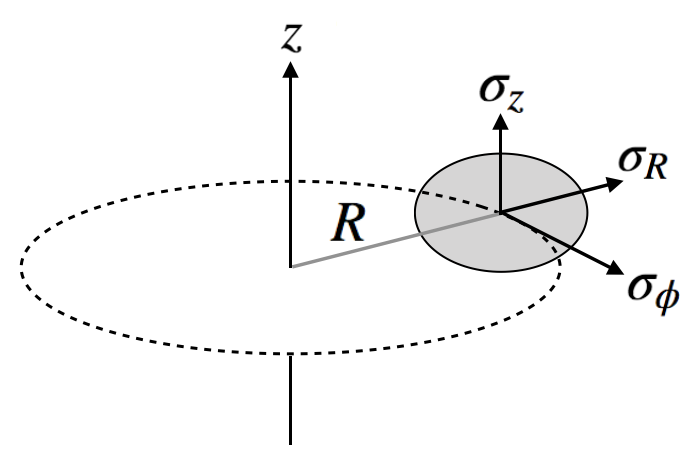
\includegraphics[width=0.8\columnwidth]{Kap2/ellipsoid.png}
  \caption{Elipsoide de velocidades en coordenadas cilíndricas}
  \label{fig:Ellipsoid}
\end{figure}


Una vez establecido detalladamente el perfil de brillo superficial, el modelo retorna el primer y segundo momentos de la velocidad y tiene como parámetros libres la anisotropía $\beta_z$ y la inclinación de la galaxia. El método también permite incluir materia oscura, agujeros negros supermasivos, anisotropía variable espacialmente y múltiples características cinemáticas.\\

A continuación se expresan las soluciones a las ecuaciones de Jeans anisotrópicas, con las suposiciones mencionadas anteriormente, que reproducen la cinemática de campo integral de galaxias reales.

%\textbf{Caso axialmente simétrico:}

Las ecuaciones (\ref{Jeans_eq_cylindric}) con el parámetro de anisotropía constante 
$$ \overline{v_R^2} = b\overline{v_z^2} $$
se reducen a:

\begin{eqnarray}
\frac{ b \nu \overline{v_R^2} - \nu \overline{v_{\phi}^2} }{R } + \frac{\partial (b \nu \overline{v_z^2})}{\partial R}  &=& -\nu \frac{\partial \Psi}{\partial R} \\
\frac{\partial (\nu \overline{v_z^2})}{\partial z}  &=& -\nu \frac{\partial \Psi}{\partial z},
\end{eqnarray}

Junto con la condición de frontera 
$$ \lim_{z\to\infty} \nu \overline{v_z^2} = 0 $$
tal que las ecuaciones de Jeans se reducen a:

\begin{eqnarray}
\label{Jeans_equation_phi}
\nu \overline{v_{\phi}^2}(R,z) &=& b \left [ R
\frac{\partial ( \nu \overline{v_z^2})}{\partial R} + \nu \overline{v_{z}^2} \right ] + R\nu \frac{\partial \Psi}{\partial R} \\
\label{Jeans_equation_z}
\nu \overline{v_z^2}(R,z)  &=& \int_z^{\infty} \nu \frac{\partial \Psi}{\partial z} dz.
\end{eqnarray}

\subsection{Método de Expansión Multi-Gaussiano (MGE)}

El brillo superficial $\Sigma$ de una galaxia puede ser parametrizado en las coordenadas del cielo $(x', y')$ a partir de la luminosidad total $L_k$ y la composición de $N$ perfiles gaussianos de luminosidad:

\begin{equation}
\label{surface_bright_cart}
\Sigma(x', y') = \sum_{k=1}^{N} \frac{L_k}{2\pi \sigma_k^2 q_k'} exp \left[ -\frac{1}{2\sigma_k^2} \left( x'^2 + \frac{y'^2}{q_k'^2} \right) \right ]
\end{equation}

con la razon axial $q'$ y dispersión $\sigma_k$ a lo largo del eje mayor. Este perfil de luminosidad debe deproyectarse para obtener la densidad volumétrica de luminosidad. La luminosidad deproyectada puede ser escrita como:

\begin{eqnarray}
\label{luminosity_density}
\nu (R,z) &=& \sum_{k=1}^{N} \frac{L_k}{(\sqrt{2\pi} \sigma_k)^3 q_k} exp \left[ -\frac{1}{2\sigma_k^2} \left( R^2 + \frac{z^2}{q_k^2} \right) \right ], \\
   &=& \sum_{k=1}^{N} \nu_{0,k} exp \left[ -\frac{1}{2\sigma_k^2} \left( R^2 + \frac{z^2}{q_k^2} \right) \right ],
\end{eqnarray}

con $$ \nu_{0,k} = \frac{ q_k' I_{0, k} }{ q_k \sqrt{2\pi} \sigma_k } $$



El método MGE describe la densidad total de masa de la misma forma que la ecuación (\ref{luminosity_density}):

\begin{equation}
\label{mass_density}
\rho (R,z) = \sum_{j=1}^{M} \frac{M_j}{(\sqrt{2\pi} \sigma_j)^3 q_j} exp \left[ -\frac{1}{2\sigma_j^2} \left( R^2 + \frac{z^2}{q_j^2} \right) \right ].
\end{equation}

En el caso auto consistente, los parámetros que describen la densidad en la ecuación (\ref{mass_density}) son equivalentes a los de la ecuación (\ref{luminosity_density})

$$ M=N \hspace{1cm} \sigma_j=\sigma_k  \hspace{1cm} q_j = q_k \hspace{1cm} M_j = \Upsilon_j L_j \hspace{1cm} \rho_j = \Upsilon_j \nu_j  $$

con $\Upsilon$ el cociente masa luminosidad para cada una de las $M (\textrm{o} L)$ componentes de masa (o luminosidad).\\


La ecuación (\ref{surface_bright_cart}) puede ser escrita en coordenadas polares en el plano del cielo $(R', \theta ')$ con la transformación:

\begin{eqnarray}
x' &=& R' cos(\theta ' - \phi) \\
y' &=& R' sin(\theta ' - \phi)
\end{eqnarray}

\begin{equation}
\label{surface_bright_polar}
\Sigma(R', \theta ') = \sum_{k=1}^{N} I_{0,k} exp \left[ -\frac{1}{2\sigma_k^2} \left( x'^2 + \frac{y'^2}{q_k'^2} \right) \right ]
\end{equation}

con $$ I_{0,k} = \frac{L_k}{ 2\pi \sigma_k^2 q_k' }, $$ 

y el término $q_k$ de planitud en la densidad de luminosidad espacial en la ecuación (\ref{luminosity_density}) está dada por:

\begin{equation}
\label{flattening}
q_k^2 = \frac{ q_k'^2 - cos^2 (i) }{ sin^2 (i) },
\end{equation}

donde $q_k'$ es la razón de ejes mayor a menor en el elipsoide bidimensional e $i$ es la inclinación de la galaxia. Sin embargo la deproyección (\ref{luminosity_density}) no es única especialmente cuando la inclinación de la galaxia $i$ es muy baja (siendo $i\approx 0$ o \emph{face on}).\\


En el caso no auto consistente, la densidad $\rho $ puede ser descrita con la suma de dos conjuntos de gaussianas: el primero de la deproyección del brillo superficial por medio de la ecuación (\ref{luminosity_density}), y el segundo por el ajuste de un modelo MGE unidimensional a alguna parametrización analitica para la materia oscura.\\

Si se resuelve la ecuación de Possion que relaciona el potencial gravitacional con la densidad de masa, se obtiene que la densidad (\ref{mass_density}) está asociada al potencial:

\begin{equation}
\label{potential_gaussians}
\Phi(R, z) = - G \frac{\sqrt{2} }{\pi} \int_0^1 \sum_{j=1}^M \frac{M_j H_j(u)}{\sigma_j} du,
\end{equation}
con
\begin{equation}
H_j(u) = \frac{exp \left \{ -\frac{u^2}{2\sigma_j^2} \left[ R^2 + \frac{z^2}{1-(1-q_j^2)U^2} \right ] \right \}  }{ \sqrt{1-(1-q_j^2)u^2 } }.
\end{equation}

Para modelar completamente el potencial de la galaxia, se usan potenciales adicionales para demás componentes de la galaxia, por ejemplo un potencial kepleriano para el agujero negro.\\



\subsection{Convolución con la PSF}

Se puede expandir la Función de Dispersión de Punto  (Point Spread Function o PSF por sus siglas en inglés ) del telescopio como una suma de $N$ gaussianas:

\begin{equation}
PSF(x', y') = \sum_{k = 1}^N \frac{G_k}{2\pi \delta_k} exp \left[ -\frac{1}{2 \delta_k^2} \left( x'^2 + y'^2 \right), \right]
\end{equation}

donde $\sum_k G_k = 1$ y $\delta_k$ son las dispersiones de las gaussianas circulares de la PSF. La distribución de brillo superficial es una convolución del brillo superficial intrínseco de la ecuación (\ref{surface_bright_polar}) con la PSF, es decir $(I * PSF)(x', y')$ que es de nuevo una suma de gaussianas y puede ser directamente ajustado a la imagen de la galaxia.


\subsection{Método MGE aplicado sobre las ecuaciones de Jeans axialmente simétricas}

Las ecuaciones de Jeans permiten modelar la cinemática de diferentes trazadores dinámicos mientras ellos se muevan en el mismo potencial. El proceso descrito en \cite{2008MNRAS.390_71C} consta de escribir las ecuaciones para las $N$ componentes gaussianas de luminosidad, donde se asume que tienen diferente anisotropía. Entonces sustituyendo las ecuaciones (\ref{luminosity_density}, \ref{potential_gaussians}) en (\ref{Jeans_equation_z}, \ref{Jeans_equation_phi}), se tiene que:

\begin{eqnarray}
\label{component_bright_vel_1}
\left[\nu \overline{v_R^2} \right]_k &=& b_k \left[\nu \overline{v_z^2} \right]_k \\
\label{component_bright_vel_2}
\left[\nu \overline{v_R^2} \right]_k &=& 4\pi G \int_0^1 \sum_{j=1}^{M} \frac{ \sigma_k^2 q_k^2 \nu_k q_j \rho_{0j} H_j(u) u^2 }{ 1-Cu^2 } du \\
\label{component_bright_vel_3}
\left[ \nu \overline{v_{\phi}^2} \right]_k &=& b_k \left[ \nu \overline{v_z^2} \right]_k + 4\pi G \int_0^1 \sum_{j=1}^{M} \frac{ \nu_k q_j \rho_{0j} H_j(u) u^2 }{ 1-Cu^2 } D R^2 du \\
\label{component_bright_vel_4}
 & = & 4\pi G \int_0^1 \sum_{j=1}^{M} \frac{ \nu_k q_j \rho_{0j} H_j(u) u^2 }{ 1-Cu^2 } (D R^2 + b_k \sigma_k^2 1_k^2) du, \\
\end{eqnarray}

con los indices $k,j$ de las densidades de luminosidad $\nu_k$ y de masa respectivamente; la densidad de masa en el origen $\rho_{0j} = \rho_j(0,0)$ y 

$$ C=1-q_j^2 - \frac{\sigma_k^2 q_k^2 }{ \sigma_j^2 } $$
$$ D = 1-b_kq_k^2 - [(1-b_k)C + (1-q_j^2)b_k ] u^2. $$

Como se indica en \cite{2008MNRAS.390_71C}, los $b_k$ no son los mismos que las componentes de luminosidad gaussianas, la anisotropía total pesada por la luminosidad en $(R, z)$ está dada por:

\begin{equation}
\label{anisotropy_z}
\beta_z(R, z) \equiv 1-\frac{ \overline{v_z^2} }{ \overline{v_R^2} } = 1-\frac{ \sum_k \left[ \nu  \overline{v_z^2} \right]  }{ \sum_k b_k \left[ \nu  \overline{v_z^2} \right] }
\end{equation}

y dado que $[\overline{v_z^2}]_k$ es una función principalmente del potencial total MGE, entonces varía relativamente poco con diferentes gaussianas y al contrario de $\nu_k$ que varía por algunos ordenes de magnitud con los componentes de luminosidad, se tiene que $[\overline{v_z^2}]_k$ es aproximadamente constante:

\begin{equation}
\label{anisotropy_z_approx}
\beta_z(R, z) \approx 1-\frac{ \sum_k \nu_k }{ \sum_k b_k \nu_k }
\end{equation}

De esta forma, la anisotropía puede ser encontrada por la el promedio de $b_k$ pesada por la luminosidad.


El modelamiento JAM expresa el trazador $n(\textbf{x})$ y la densidad de brillo $\nu(R, z)$ en términos de la Expansión Multi-Gaussiana. Éstas cantidades se asume son proporcionales.\\

Con los modelos MGE y JAM se puede recuperar el tensor de dispersión de velocidades de manera univoca \cite{TR16}, donde se tiene que: $\overline{v_i v_j}(R,z) = \overline{v_i^2}(R, z)$ para las coordenadas cilíndricas y $\overline{v_i v_j} = 0$ si $i\neq j$. Para compararlo con las observaciones, $\overline{v_i^2}(R, z)$ debe ser rotado un ángulo $i$ en el sistema de coordenadas del observador $(x', y')$ del plano del cielo, $x'$ alineado con el eje mayor de la galaxia y $z'$ en la línea de visión del observador.\\

De esta forma, la proyección pesada por la luz da la predicción del segundo momento de la velocidad en la línea de visión $\overline{v_{los}^2}(x', y')$ que es comparable con las mediciones espectroscópicas del segundo momento de la velocidad.

\subsection{Integración en la línea de visión del segundo momento de la velocidad}

Las cantidades intrínsecas tienen que ser integradas a lo largo de la línea de visión para generar los observables que pueden ser comparados con la cinemática de la galaxia. Como se mencionó las coordenadas primadas son en el plano de la galaxia y su relación con las coordenadas de la galaxia $(x, y, z)$ está dada por una rotación en torno al eje $x'$ y el eje $z'$ coincide con el eje de simetría de la galaxia:

\[
\begin{bmatrix}
    x \\
    y \\
    z
\end{bmatrix}
=
\begin{bmatrix}
    1 & 0 & 0 \\
    0 & -cos(i) & sin(i) \\
    0 & sin(i) & cos(i)
\end{bmatrix}
\begin{bmatrix}
    x' \\
    y' \\
    z'
\end{bmatrix}.
\]

El segundo momento de la velocidad a lo largo del la línea de visión $\overline{v_{los}^2} \equiv \overline{v_z^2}$, para una componente gaussiana de luminosidad, está dada por:

\begin{equation}
\left[ \Sigma v_{los}^2 \right]_k = \int_{-\infty}^{\infty} \left \{ \left[  \nu \overline{v_{z}^2} \right]_k  cos^2 (i) + \left( \left[ \nu \overline{v_{R}^2} \right]_k sin^2 (\phi) + \left[ \nu \overline{v_{\phi}^2} \right]_k cos^2 (\phi) \right ) sin^2 (i) \right \} dz',
\end{equation}

donde $cos(\phi) = x/R$, y el segundo momento de toda la expansión MGE es:

\begin{equation}
 \Sigma \overline{v_{los}^2} = \sum_{k = 1}^N \left[ \Sigma \overline{v_{los}^2} \right]_k ,
\end{equation}

luego de la sustitución de las ecuaciones (\ref{component_bright_vel_1}, \ref{component_bright_vel_4}), la integral en $z'$ puede ser escrita y sumando sobre las $N$ componentes gaussianas, se obtiene \cite{2008MNRAS.390_71C}:


\begin{eqnarray}
\label{v_los_sky_plane}
\Sigma \overline{v_{los}^2}(x', y') &=& 4\pi^{3/2} G \int_0^1 \sum_{k=1}^N \sum_{j=1}^M \nu_{0,k} q_j \rho_{0,j} u^2 \\
    &\times & \frac{ \sigma_k^2 1_k^2(cos^2(i) + b_k sin^2(i)) + Dx'^2 sin^2(i) }{ (1-Cu^2) \sqrt{ (A+B cos^2 (i) ) [ 1-(1-q_j^2)u^2 ] } } \\
  & \times & \left \{  -A\left[ x'^2 + \frac{(A+B)y'^2}{ A+Bcos^2(i) } \right]  \right \} du,
\end{eqnarray}

donde se ha definido $\nu_{0,k}=\nu_k(0,0)$ y

\begin{eqnarray}
A &=& \frac{1}{2} \left( \frac{u^2}{\sigma_j^2} + \frac{1}{\sigma_k^2}  \right) \\
B &=& \frac{1}{2} \left\{ \frac{1-q_k^2}{\sigma_k^2 q_k^2} + \frac{(1-q_j^2)u^4 }{\sigma_j^2 \left[ 1-(1-q_j^2)u^2 \right] }  \right\}.
\end{eqnarray}

El caso semi-isotrópico se puede reproducir por $b_k = 1$ y $M_k = \Upsilon L_k$. La ecuación (\ref{v_los_sky_plane}) puede ser deducida directamente del ajuste al brillo superficial de la galaxia sin tener que hacer la deproyección o la deconvolución con la PSF, y permite modelar así galaxias con anisotropía variable, múltiples componentes cinemáticos.\\


De acuerdo al trabajo de Cappellari \cite{2008MNRAS.390_71C} se observa (en figura \ref{fig:NGC2974}) la variación de los segundos momentos de la velocidad LOS $\overline{v_{LOS}^2}^{1/2}$  por cambios en la inclinación $i$ y el factor de anisotropía $\beta_z$ para datos de Espectroscopía de Campo Integral (IFU - \emph{Integral Field Spectroscopy}) del catálogo SAURON. Los valores de mejor ajuste para la razón masa luminosidad $\Upsilon$ están dados para cada par de parámetros $i, \beta_z$.\\


\begin{figure}
  \centering
    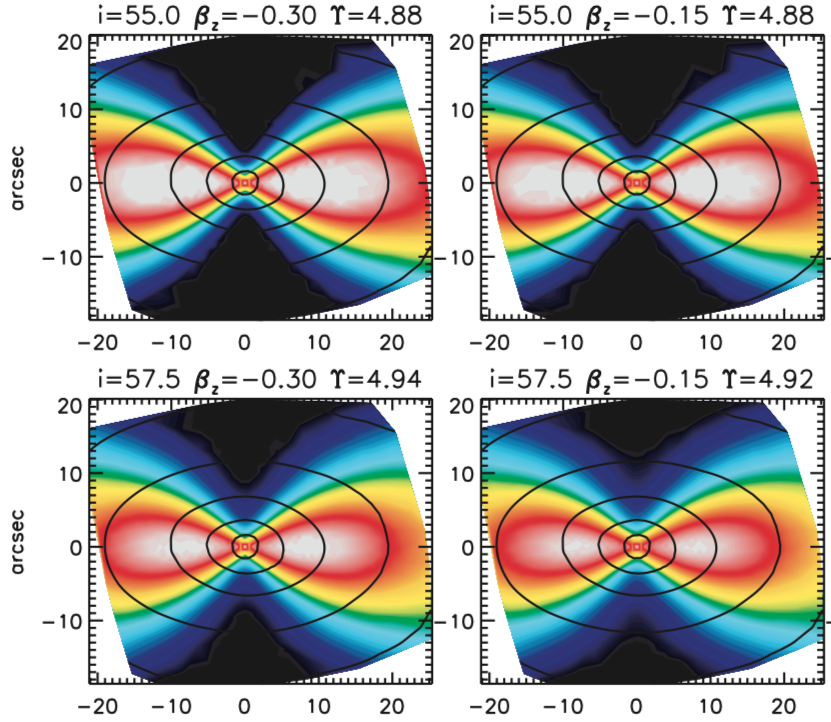
\includegraphics[width=0.45\columnwidth]{Kap2/NGC2974_1.png}
    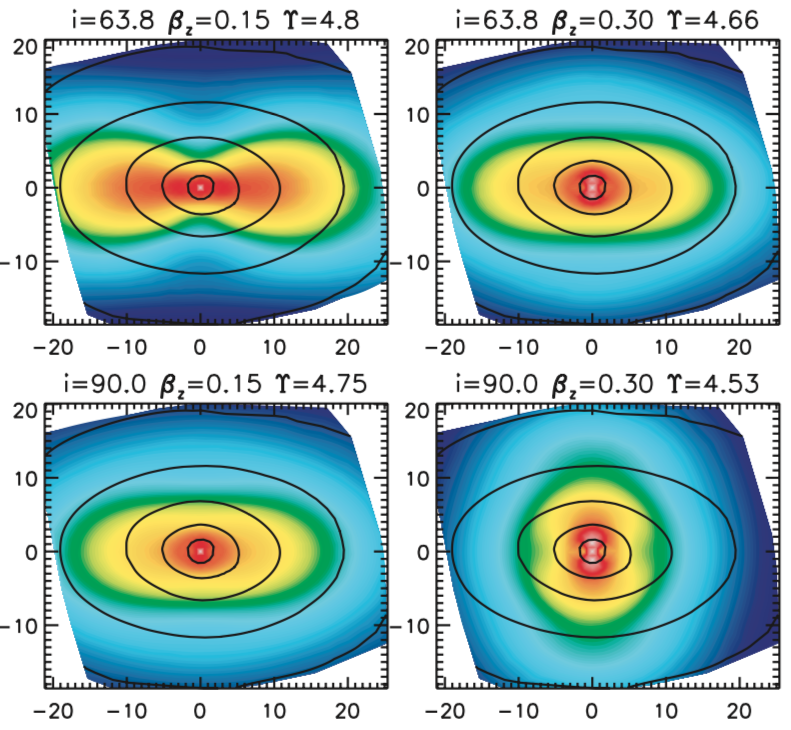
\includegraphics[width=0.45\columnwidth]{Kap2/NGC2974_2.png}
  \caption{Variación de la inclinación $i = 55.0, 57.5, 63.8, 90.0$ y factor de anisotropía $\beta_z = -0.30, -0.15, 0.15, 0.30$ para la galaxia NGC 2974. Se muestran los campos de los segundos momentos de la velocidad LOS $\overline{v_{LOS}^2}^{1/2}$. Tomado de \cite{2008MNRAS.390_71C}}
  \label{fig:NGC2974}
\end{figure}

Los segundos momentos en la ecuación (\ref{v_los_sky_plane}) son una buena aproximación para la cantidad observada $V_{rms} = V^2 + \sigma^2$, donde $V$ es la velocidad estelar media y $\sigma$ la dispersión de velocidades. Un campo de velocidades de $V_{rms}$ y $V$ para el catálogo SAURON se muestra en la figura   \ref{fig:NGC2974_2}.

\begin{figure}
  \centering
    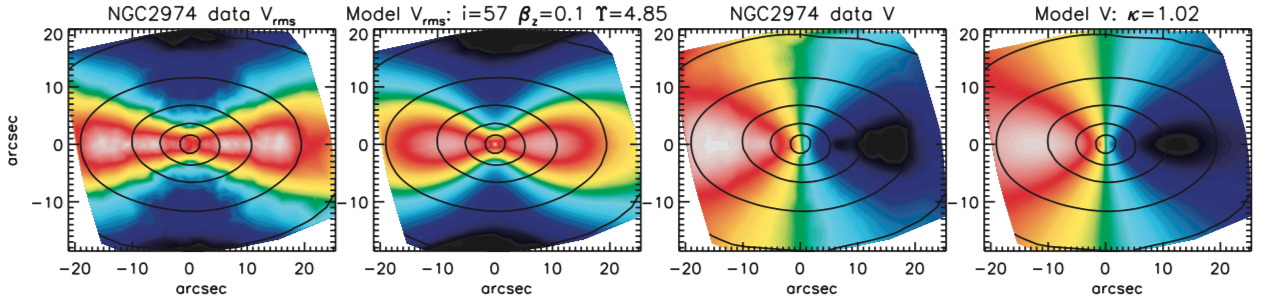
\includegraphics[width=0.95\columnwidth]{Kap2/NGC2974_3.png}
  \caption{De izquierda a derecha se muestran los datos $V_{rms}$ de los datos SAURON, el mejor ajuste del modelo para $\overline{v_{LOS}^2}^{1/2}$, los datos $V$ de SAURON y el mejor ajuste del modelo para el primer momento $\overline{v_{LOS}}$. Tomado de \cite{2008MNRAS.390_71C}}
  \label{fig:NGC2974_2}
\end{figure}


\section{Modelamiento dinámico con simetría esférica - \emph{Jeans Anisotropic Models} (JAM)}

El caso axialmente simétrico visto en la sección anterior no reproduce la dinámica de galaxias elípticas que rotan lentamente. Los modelos mas realistas y generales están basados en que son triaxiales y basados en partículas o en órbitas. En el caso de la aproximación triaxial, se tiene una degeneración que no permite obtener una solución única a las ecuaciones de Jeans.\\

Un modelo mas simple consiste en que las isofotas proyectadas, de sistemas rotantes lentos, son aproximadamente circulares especialmente en la parte central donde se conoce la cinemática observacionalmente, lo cual indica que el sistema no está muy lejos de ser esférico \cite{2008MNRAS.390_71C}. Con esta consideración se puede sugerir un modelo esférico como una aproximación a primer orden de por lo menos algunos objetos.\\

\subsection{Solución general}

De la ecuación de Boltzmann sin colisiones en coordenadas esféricas se obtuvo las ecuaciones de Jeans en simetría esférica:

\begin{equation}
\label{Jeans_spheric_r}
\frac{d \nu \overline{ v_r^2 } }{ dr } + \frac{2 \beta \nu \overline{ v_r^2 } }{r} = -\nu \frac{ d \Phi }{dr},
\end{equation}
donde se ha considerado $\overline{ v_{\theta}^2 } = \overline{ v_{\phi}^2 }$ por simetría y con el parámetro de anisotropía 

$$\beta = 1- \frac{ \overline{ v_{\theta}^2 } }{ \overline{ v_r^2 } }. $$

La solución a la ecuación de Jeans (\ref{Jeans_spheric_r}) con anisotropía constante y con la condición de frontera
$$ \nu \overline{ v_r^2 } = 0, \hspace{2 cm} r \rightarrow \infty $$

está dada por:

\begin{eqnarray}
\nu \overline{ v_r^2 } (r) &=& r^{-2\beta} \int_r^{\infty} \nu(u) \frac{d\Phi}{du} u^{2\beta} du \\
 &=& G r^{-2\beta} \int_r^{\infty} \frac{\nu(u) M(u) }{ u^{2-2\beta} } du,
\end{eqnarray}

con $$ \frac{d\Phi}{dr} = G \frac{M}{r^2}. $$

Proyectando a lo largo de la línea de visión (LOS) $z'$, se obtiene el segundo momento de la velocidad:

\begin{eqnarray}
\Sigma \overline{v_{los}^2} (R) &=& 2 \int_R^{\infty} \left (  1-\beta \frac{R^2}{r^2}  \right ) \frac{\nu \overline{ v_r^2 }(r) r }{ \sqrt{r^2 - R^2} } dr \\
 &=& 2G \int_R^{\infty} \left [  \frac{r^{-1-2\beta}(r^2-R^2\beta) }{\sqrt{r^2 - R^2} }  \int_r^{\infty} \frac{\nu(u) M(u) }{ u^{2-2\beta} } du \right ] dr,
\end{eqnarray}

donde $R$ es el radio proyectado, medido desde el centro de la galaxia. Integrando por partes, la doble integral puede ser reducida a una única cuadratura, involucrando funciones especiales:

\begin{equation}
\label{sigma_los_spherical}
\Sigma \overline{v_{los}^2} (R) = 2G \int_R^{\infty} \frac{ F(r) \nu(r) M(r) }{ r^{2-2\beta} } dr,
\end{equation}

donde

\begin{equation}
\label{F_r}
F(r) = \frac{R^{1-2\beta}}{2} \left [ \beta B_{\omega} \left( \beta + \frac{1}{2}, \frac{1}{2} \right)-B_{\omega} \left( \beta - \frac{1}{2}, \frac{1}{2} \right) +\frac{ \pi(3-2\beta) \Gamma (\beta - 1/2) }{ 2\Gamma (\beta) }  \right ],
\end{equation}

con $\omega = (R/r)^2$ , $B_{\omega} $ es la función Beta incompleta y el límite isotropico

$$ \lim_{\beta\to 0} F(r) = \sqrt{r^2 - R^2} $$

\subsection{Método MGE aplicado sobre las ecuaciones de Jeans esféricamente simétricas}

De forma análoga al procedimiento para la simetría axial, se parametrizan la densidad de luminosidad y la densidad total de masa, pero en este caso con $q_j = q_k = 1$ considerando la simetría esférica.
Para una sola gaussiana:

\begin{eqnarray}
\Sigma_k (R) &=& \frac{ L_k }{ 2\pi \sigma_k^2 } exp \left( -\frac{R^2}{2\sigma_k^2} \right)\\
\label{luminosity_density_spherical}
\nu_k (r) &=& \frac{ L_k }{ (\sqrt{2\pi} \sigma_k)^3 } exp \left( -\frac{r^2}{2\sigma_k^2} \right)\\
\rho_j (r) &=& \frac{ M_j }{ (\sqrt{2\pi} \sigma_j)^3 } exp \left( -\frac{r^2}{2\sigma_j^2} \right),\\
\end{eqnarray}

Así, la masa contenida en un radio $r$ es:

\begin{equation}
\label{mass_component_radius}
M_j (r) = M_j \left[ erf \left( \frac{r}{\sqrt{2}\sigma_j } \right) -\frac{ \sqrt{2/\pi} r }{\sigma_j } exp \left( -\frac{r^2}{2\sigma_j^2} \right)   \right],
\end{equation}

donde $erf (x)$ es la función error. \\

Con la ecuación (\ref{sigma_los_spherical}) y la superposición, de los segundos momentos de velocidad LOS proyectada, en todas las componentes de luminosidad:

$$ \Sigma \overline{v_{los}^2} = \sum_{k=1}^N \left[ \Sigma \overline{v_{los}^2} \right]_k, $$

se tiene que el segundo momento de la velocidad proyectado para todo el modelo MGE es:
\begin{equation}
\label{vel_los_spherical}
\Sigma \overline{v_{los}^2} (R) = 2G \int_R^{\infty} \sum_{k=1}^N \frac{F_k(r) \nu_k(r) }{ r^{2-2\beta_k} }  \left[ M_* + \sum_{j=1}^M M_j(r) \right] dr,
\end{equation}

con $\nu_k (r)$ dado por la ecuación (\ref{luminosity_density_spherical}), $M_j(r)$ por (\ref{mass_component_radius}) y $F_k(r)$ calculada remplazando $\beta$ en (\ref{F_r}), $M_*$ la masa de un agujero negro supermasivo y de esta forma la ecuación (\ref{vel_los_spherical}) involucra solo una integral para modelar objetos aproximadamente esféricos con un perfil de anisotropía variable, una razón masa-luminosidad variable, un objeto central galáctico y un perfil de materia oscura.




\section{\emph{Software} disponible}

\subsection{galpy}

\textsc{galpy}\footnote{Ver: http://galpy.readthedocs.io/en/latest/\#} es una biblioteca escita en \verb+python+ que contiene un conjunto de herramientas para dinámica galáctica, incluyendo potenciales gravitacionales y cantidades derivadas de éste como la densidad de masa, velocidad circular, masa total, entre otros. \textsc{galpy} realiza integración numérica de órbitas con una variedad de integradores simplecticos y Runge-Kuta. Soporta el cálculo de coordenadas acción angulo y frecuencias orbitales para potenciales esféricos. Por otra parte \textsc{galpy} incluye funciones de distribución en dos dimensiones para discos con y sin simetría axial, en tres dimensiones para discos y funciones de distribución para corriente de marea \cite{B15}. Finalmente, \textsc{galpy} es consistente en el uso de sistemas de unidades en física astronomía y tiene una adecuada interfaz gráfica. Algunos ejemplos se ilustran en la figura (\ref{fig:Fi1})

\begin{figure}
  \centering
    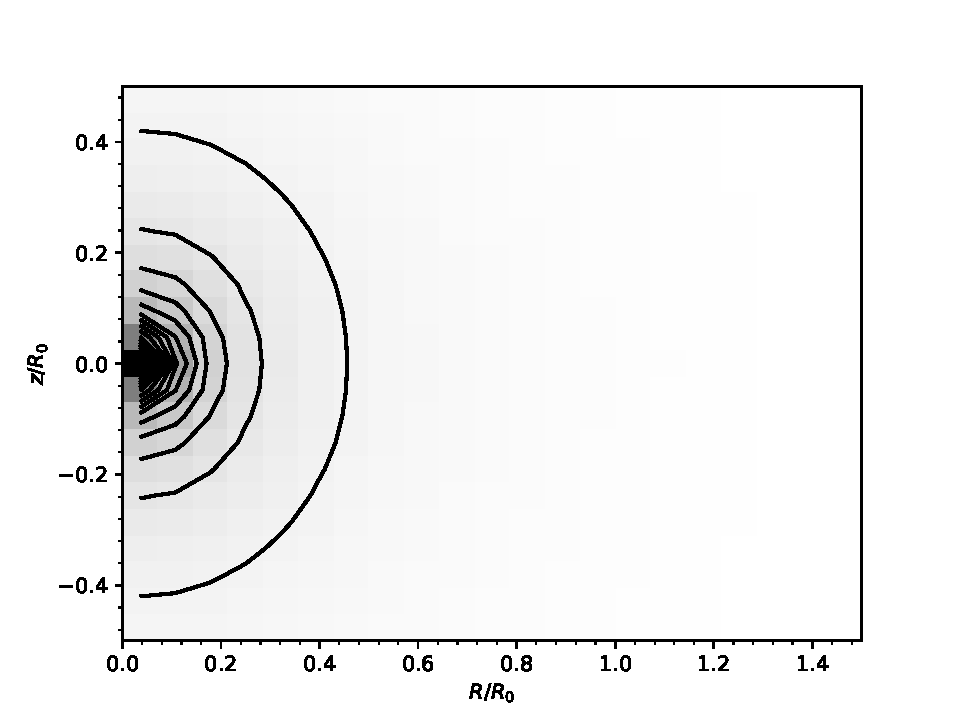
\includegraphics[width=0.4\columnwidth]{Kap2/Bulge.pdf}
    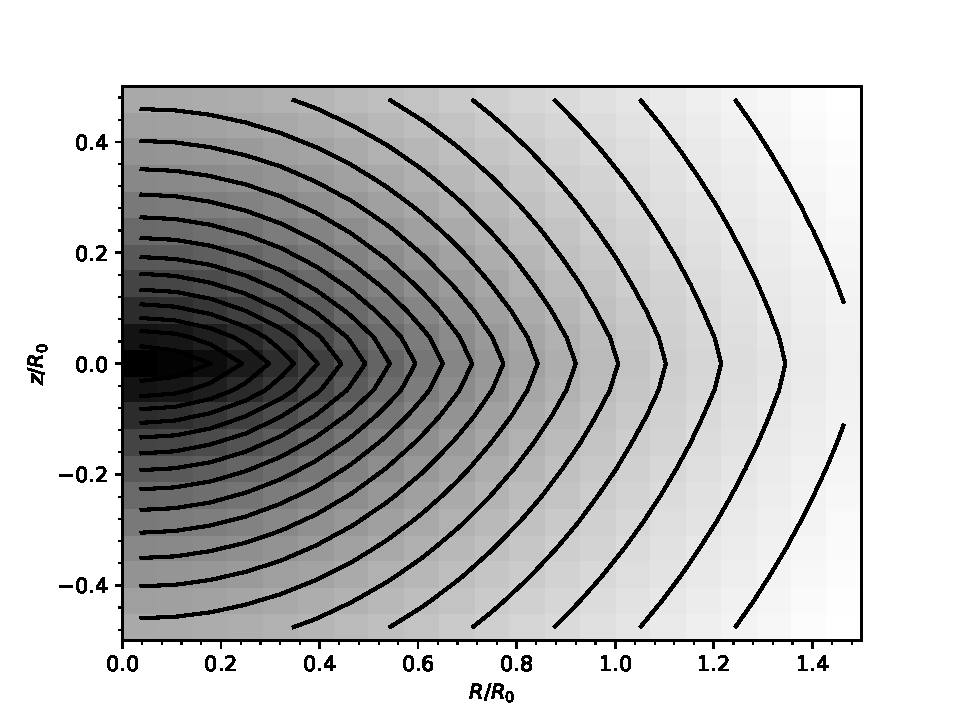
\includegraphics[width=0.4\columnwidth]{Kap2/TnDisk.pdf}
  \caption{Densidad de masa para un bulbo y un disco con modelos Miyamoto-Nagai (gráficas por \textsc{galpy})}
  \label{fig:Fi1}
\end{figure}

\subsection{GalRotpy}

Basado en las funciones de \textsc{galpy}, \textsc{GalRotpy}\footnote{https://github.com/andresGranadosC/GalRotpy.git} ofrece un entorno diseñado para ajustar una curva de rotación dada por medio de la parametrización del potencial gravitacional usando las rutinas de potenciales gravitacionales de \textsc{galpy}.\\

\textsc{GalRotpy} requiere unos valores iniciales y umbrales para los parámetros de los potenciales gravitacionales, de la galaxia en estudio, en un archivo \verb+input_params.txt+. Éste archivo debe contener un valor central para la masa (en unidades  M$_\odot$), distancia galactocéntrica (en kpc) y sus umbrales asociados en los cuales se espera que estén los parámetros de cada potencial. El umbral debe ser dex del estimado de masa ($M$) y un porcentaje \% para las escalas radial y de altura $a$ y $b$.

Se requieren los siguientes paquetes de \verb+python+ para usar \textsc{GalRotpy}: \verb+matplotlib+ para generar la interfaz gráfica, \verb+astropy+ y \textsc{galpy}.\\


De acuerdo a la figura \ref{fig:GUI1}, en el panel izquierdo se muestra una lista de verificación para seleccionar los potenciales a incluir en la curva de rotación resultante compuesta. La contribución de masa y escalas de tamaño para cada modelo tienen una guía roja que muestra el valor de inicio y umbral que se introdujo en  el archivo \verb+input_params.txt+.

\begin{figure}
  \centering
    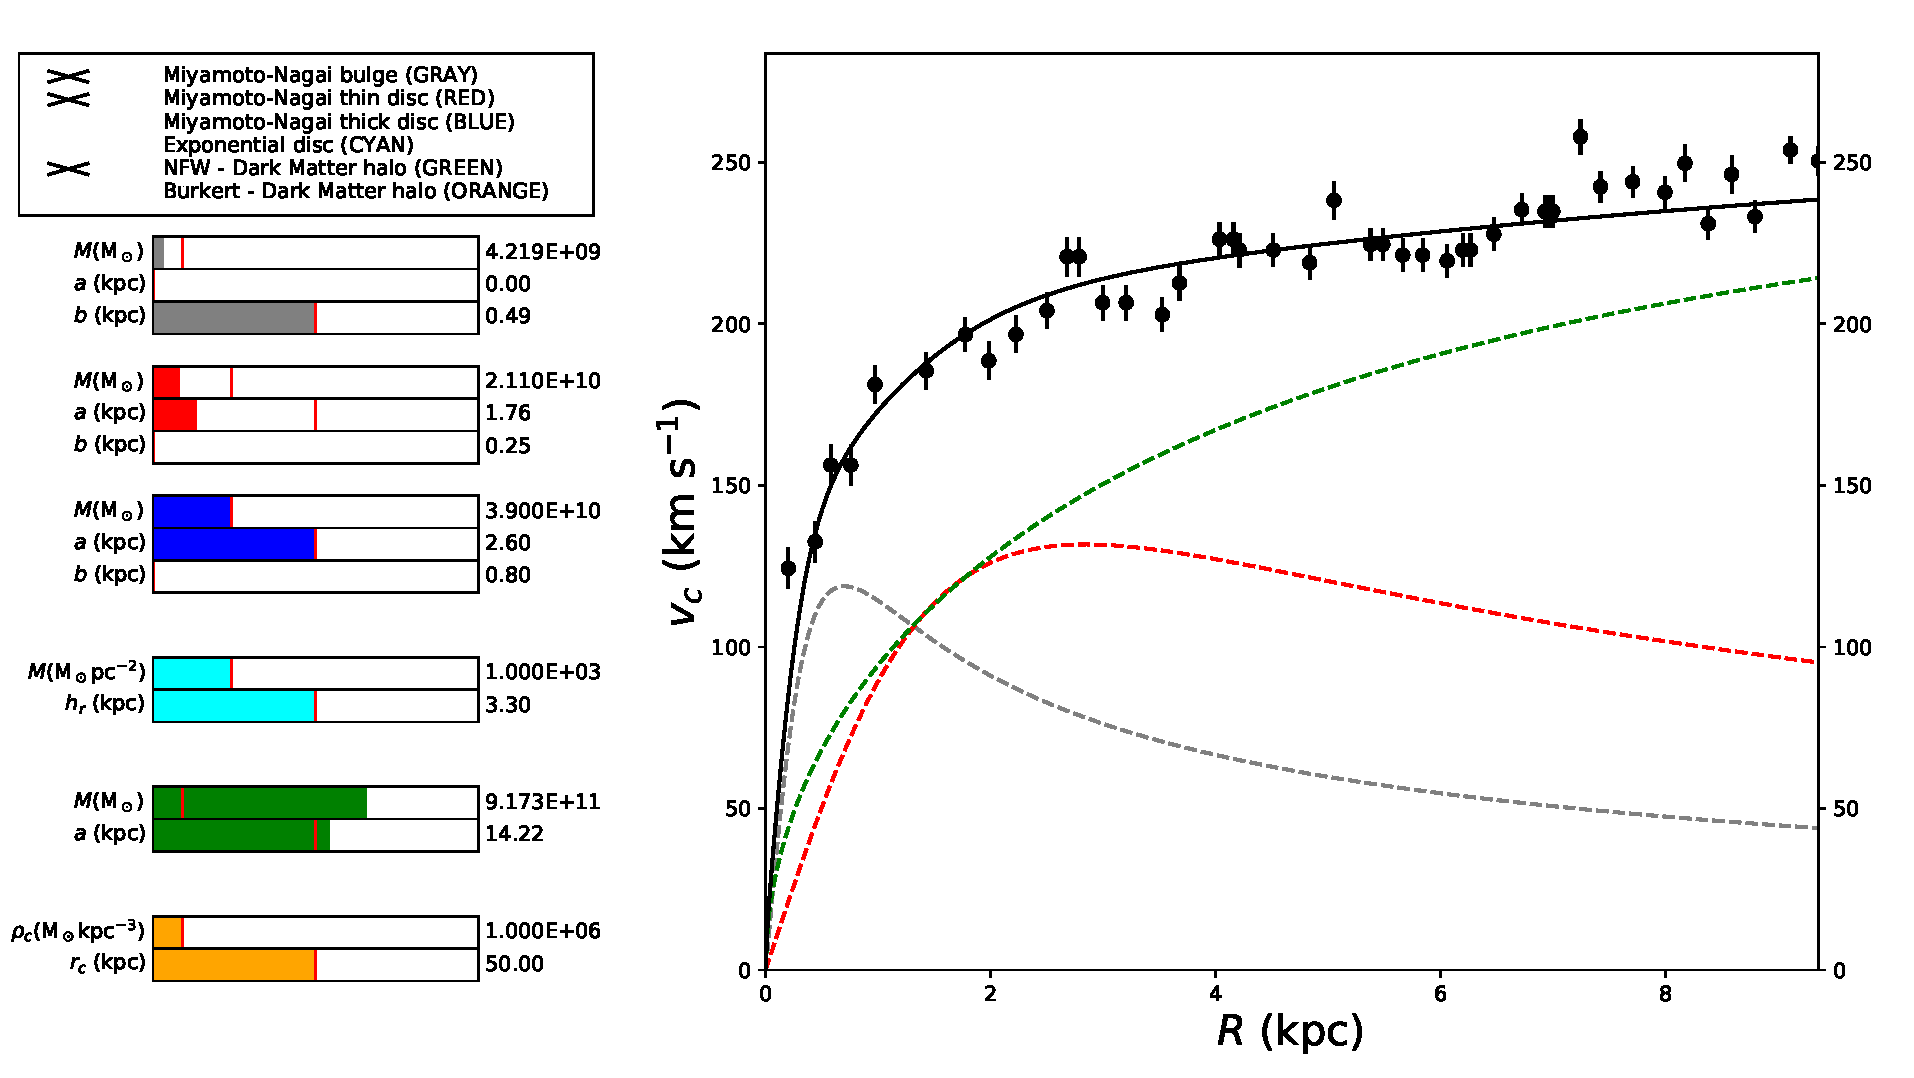
\includegraphics[trim=0cm 0cm 22cm 0cm,clip=true, width=0.4\columnwidth]{Kap2/curve_RotPy.pdf}
    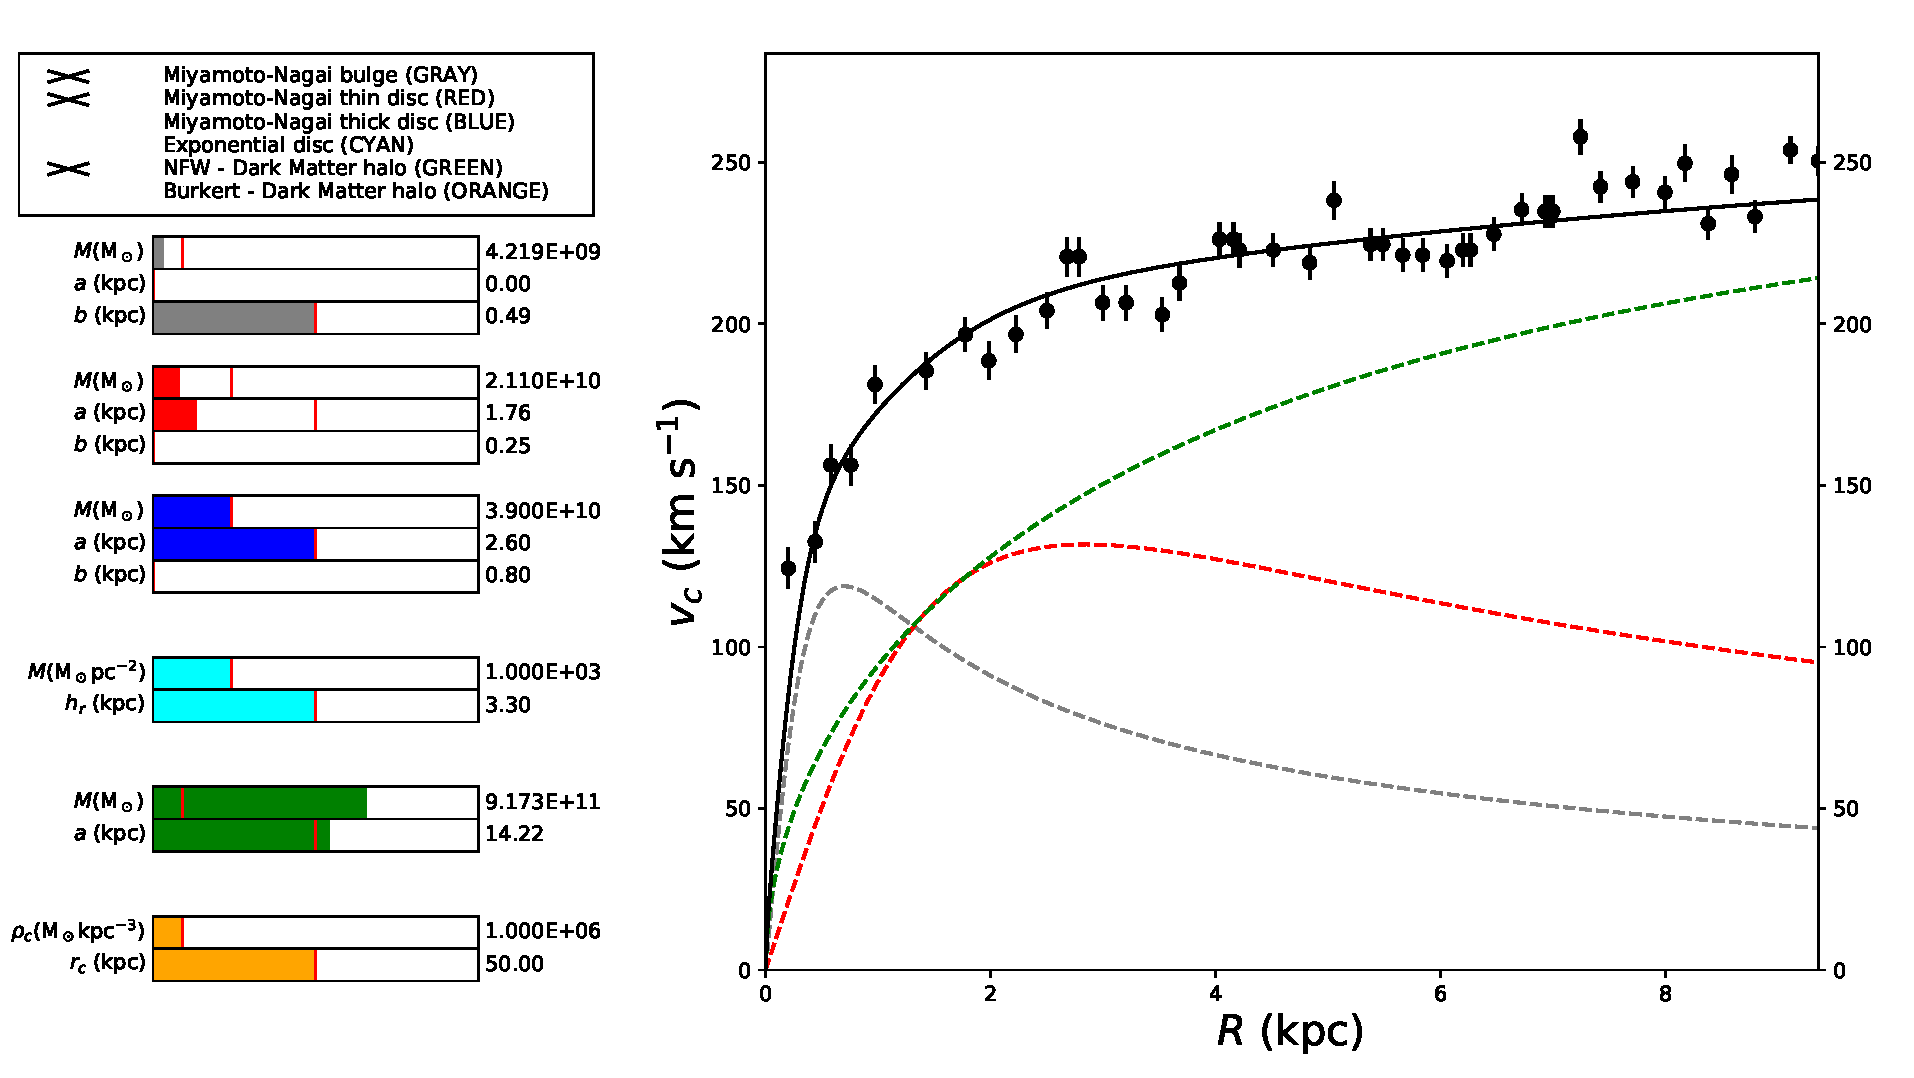
\includegraphics[trim=10.5cm 0cm 0cm 0cm,clip=true, width=0.6\columnwidth]{Kap2/curve_RotPy.pdf}
  \caption{ Panel para la selección y ajuste de parámetros de cada potencial gravitacional (arriba) y su composición de la curva de rotación (abajo)}
  \label{fig:GUI1}
\end{figure}

La curva de rotación debe ser un archivo llamado \verb+rot_curve.txt+ que contiene tres columnas con unidades kiloParsec (kpc) para la coordenada radial y kilometros por hora (km  s$^{-1}$) para la velocidad y su incertidumbre.\\

Los controles deslizantes en el panel de la izquierda permiten calcular, en tiempo real, la velocidad circular en correspondencia a los potenciales seleccionados, mostrados en líneas punteadas de colores diferentes. La línea sólida negra describe la curva de rotación resultante. 

Luego del ajuste visual del modelo dinámico, cuando la interfaz de \textsc{GalRotpy} se cierra, es generada una lista \verb+output_parameters.txt+ de parámetros para el conjunto de potenciales seleccionados. Esta lista contiene el modelo dinámico para la galaxia en estudio de acuerdo a su curva de rotación.\\

En \cite{2017arXiv170501665G} se muestran los resultados para dos galaxias espirales de prueba: las galaxias NGC6361 (figura \ref{fig:Fi4}) y M33 (figura \ref{fig:FigM33RC}). \textsc{GalRotpy} en primera aproximación permite obtener la dinámica de la galaxia tipo disco y :

\begin{itemize}
\item verificar rápidamente la presencia de una componente de masa en una curva de rotación observada para construir un modelo dinámico, incluyendo o removiendo un potencial;
\item determinar cuantitativamente la principal contribución de masa en una galaxia usando principalmente la razón de masas del bulbo respecto del disco o del disco respecto a la Materia Oscura;
\item acotar la extensión de cada componente de masa dada su escala radial o de altura. Los parámetros del potencial gravitacional como resultado del ajuste de la curva de rotación revela la distribución de masa en la galaxia;
\item evidenciar la influencia de las principales componentes de masa de la galaxia en la totalidad del sistema estelar gravitante.
\end{itemize}





\begin{figure}
  \centering
  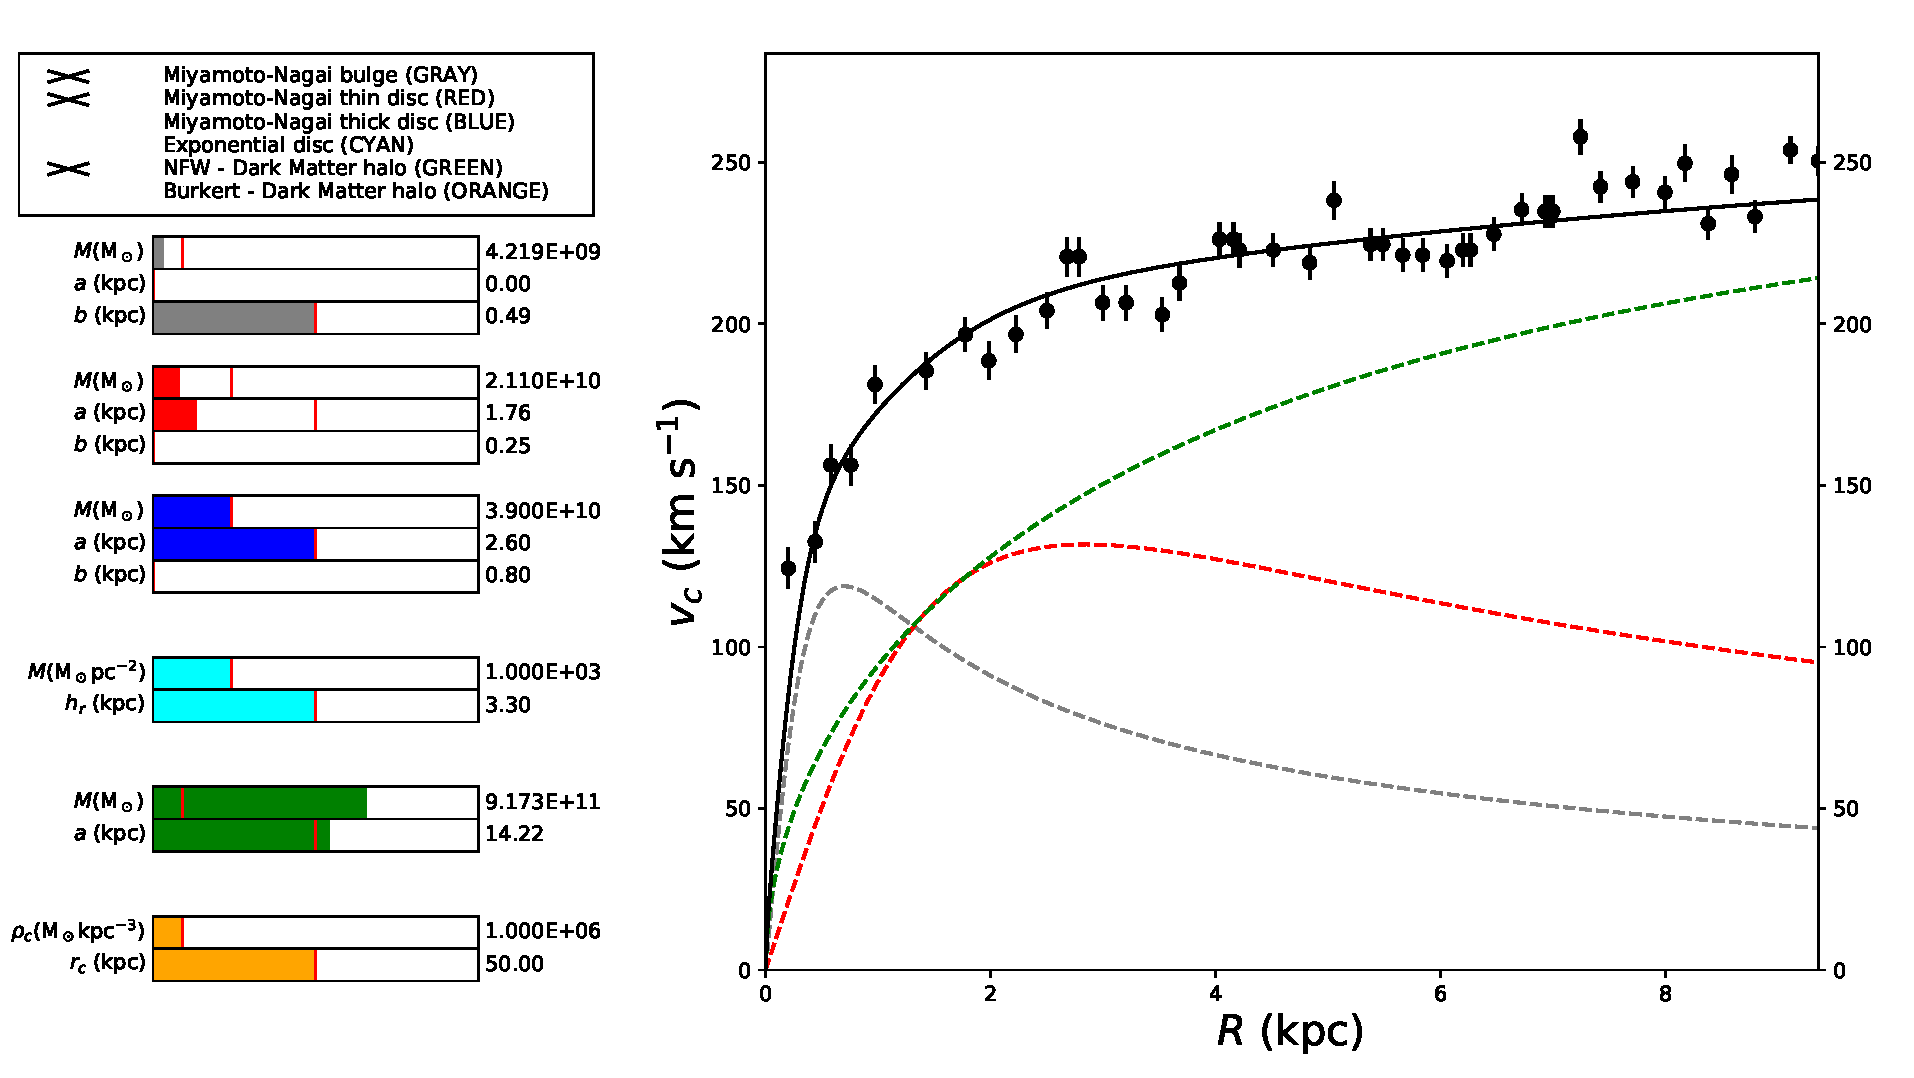
\includegraphics[width=\columnwidth]{Kap2/curve_RotPy.pdf}
  \caption{Una composición a la curva de rotación de la galaxia espiral  NGC6361, con un bulbo, un disco delgado y un halo de Materia Oscura}
  \label{fig:Fi4}
\end{figure}


\begin{figure}
  \centering
    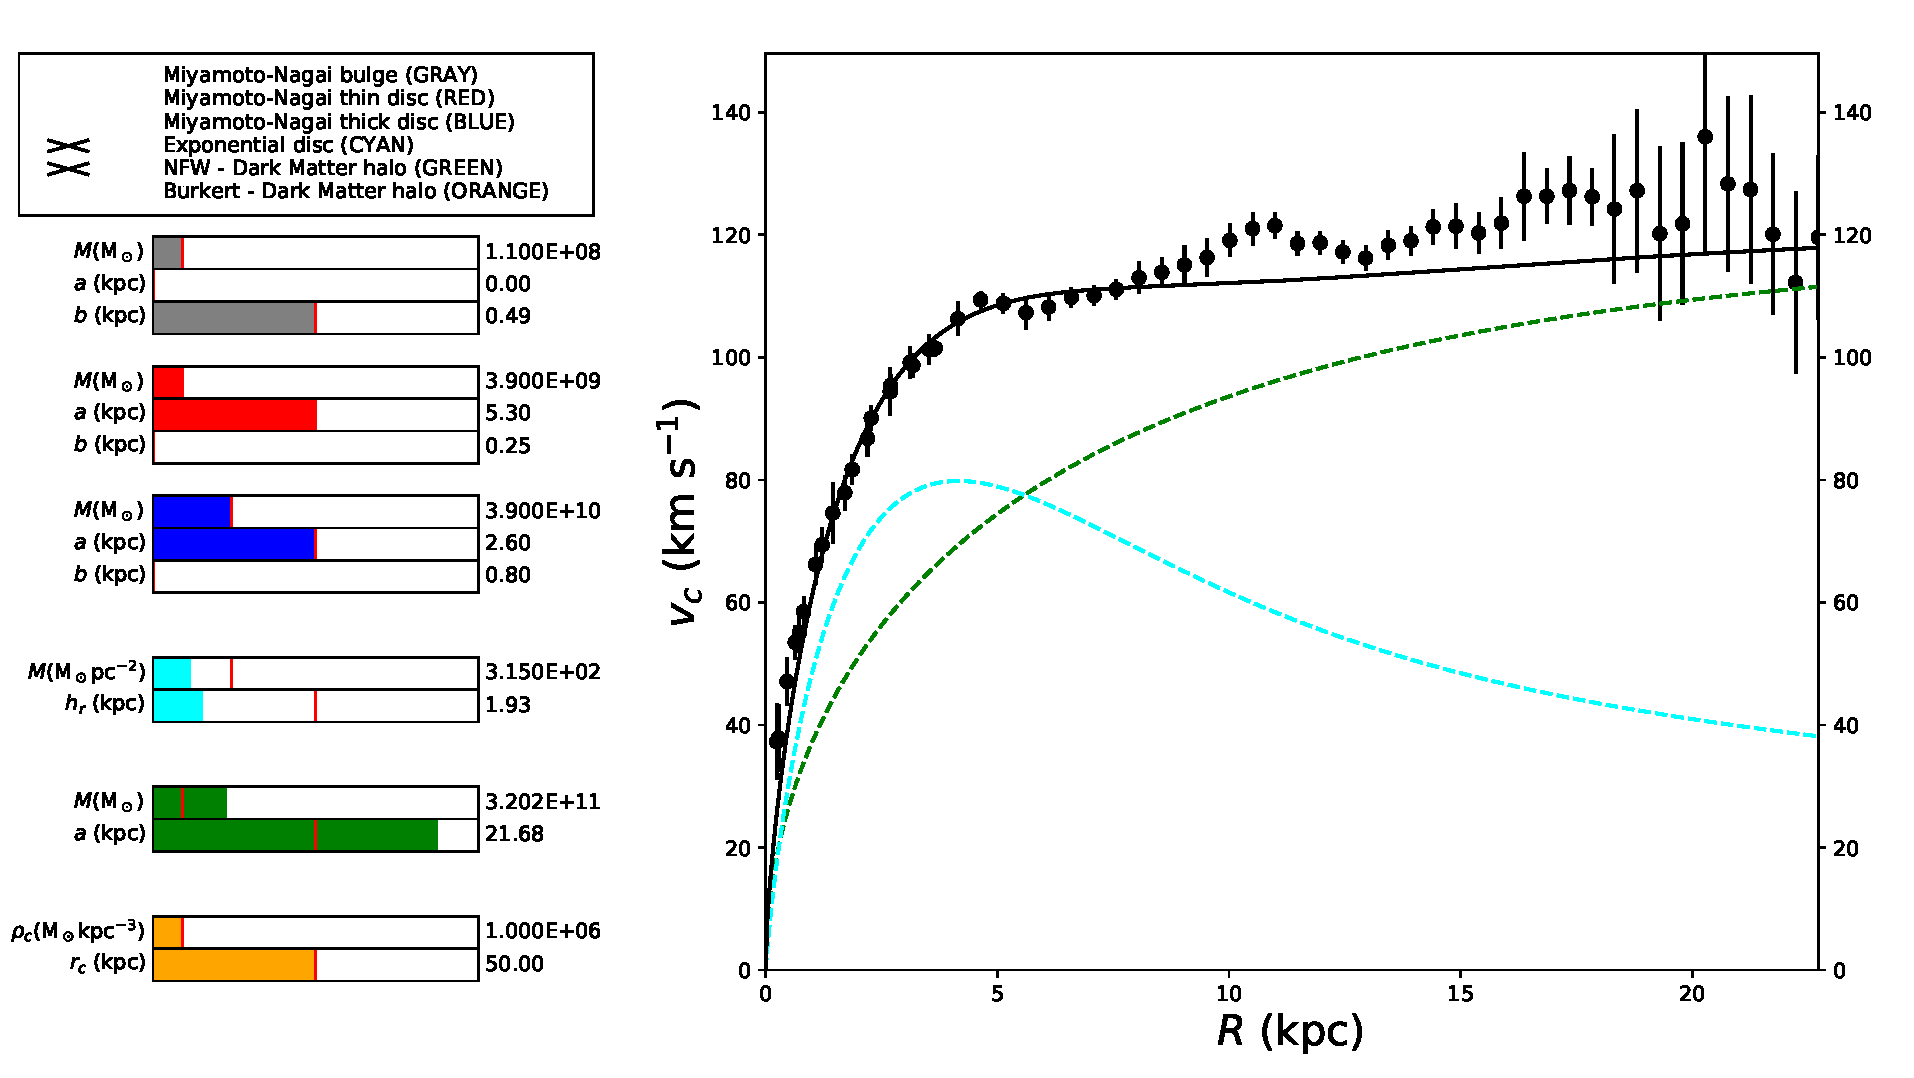
\includegraphics[width=\columnwidth]{Kap2/M33_rot_curve.pdf}
    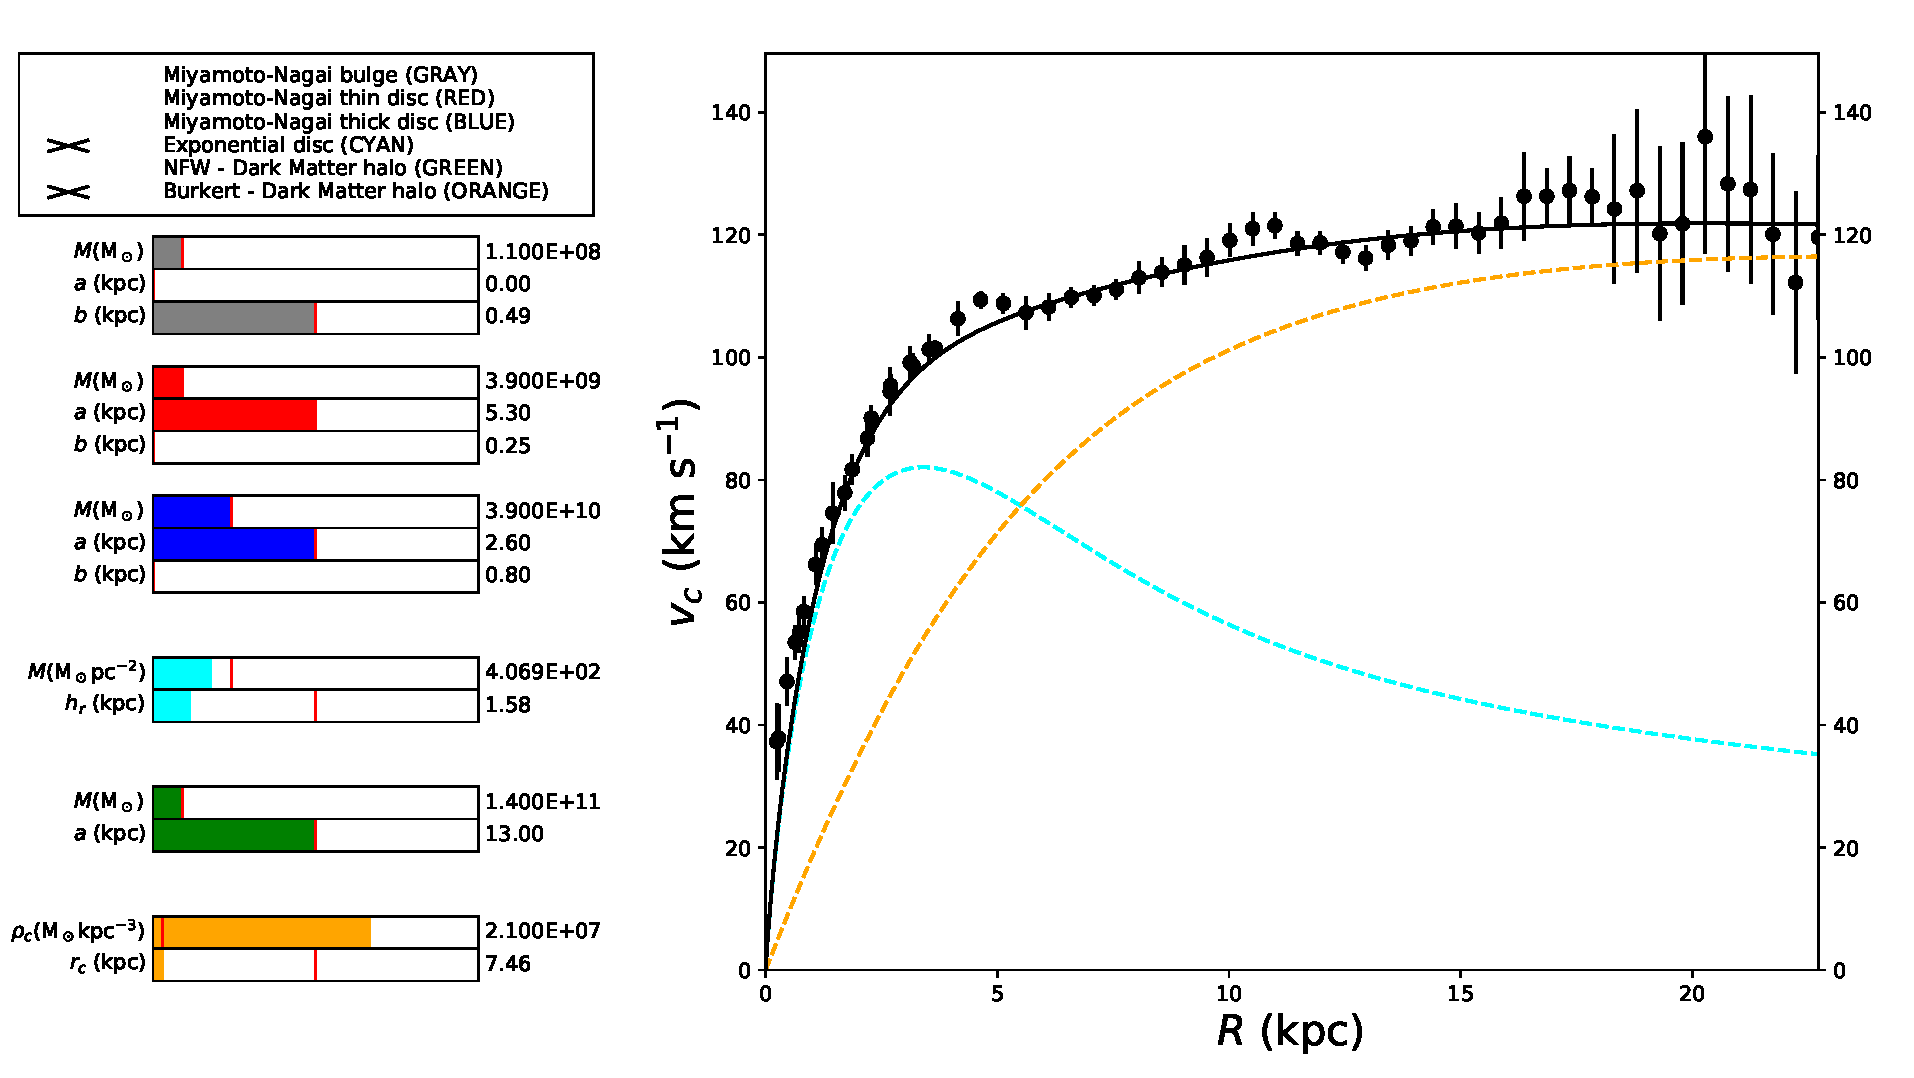
\includegraphics[width=\columnwidth]{Kap2/M33_Burkert.pdf}
  \caption{La curva de rotación resultante para la galaxia M33, usando un modelo NFW (arriba) y un modelo de Burkert (abajo) para el halo de Materia Oscura. La curva de rotación fue tomada de \cite{C14}}
  \label{fig:FigM33RC}
\end{figure}



\subsection{lenstronomy - GalKin}

\verb+lenstronomy+ es un paquete escrito en \verb+Python+ que contiene herramientas para modelar el efecto de lente gravitacional fuerte, de las cuales se muestran las mas relevantes:

\begin{itemize}
\item modelar una superposición arbitraria de lentes gravitacionales
\item resolver la ecuación de lente
\item modelamiento cinemático
\end{itemize}

El desarrollo del paquete \verb+lenstronomy+ está basado en \cite{BI15}. Algunos de los módulos se listan a continuación:

\begin{itemize}
\item \verb+LensModel+: contiene las funcionalidades de lentes gravitacionales. Resolver la ecuación de lente, cálculo del tiempo de llegada y solucionadores no lineales para optimizar los modelos de lente para configuraciones de imagen particulares
\item \verb+LightModel+: para describir el brillo/masa superficial de la galaxia como una superposición de perfiles definidos analíticamente o en una base \emph{shapelets}. Contiene perfiles gaussiano, hernquist, pseudo - Jaffe, Sersic, torus (elipse con brillo superficial constante), uniforme (gaussiano)
\item \verb+PointSource+: para predecir y modelar exactamente las posiciones y flujos de fuentes puntuales.
\end{itemize}

El módulo \verb+GalKin+ calcula la cinemática estelar de la galaxia deflectora con modelamiento de las ecuaciones de Jeans basado en el modelo de masa que se usó en LensModel y en el modelo de brillo definido en \verb+LightModel+.

\verb+GalKin+ modela consistentemente la velocidad de dispersión de la galaxia lente dado el perfil de brillo superficial basado en la imagen de la galaxia. Para esto se requiere un conocimiento del perfil 3D de brillo y masa. No todas las lentes y modelos de brillo pueden ser de-proyectados analíticamente. En esos casos, lenstronomy realiza descomposición multi-gaussiana y la de-proyección es realizada en componentes gaussianas individuales.

\subsection{Kinemetry}

El paquete \textsc{Kinemetry}\footnote{http://davor.krajnovic.org/idl/} escrito en \textsc{IDL} que permite analizar mapas 2D de los segundos momentos de la velocidad en la línea de visión (LOSVD Line-Of-Sight Velocity Distribution) como es descrito en \cite{2006MNRAS.366..787K}. El método en el cual se basa el software es una generalización de la fotometría superficial de todos los momentos de la LOSVD. Se hace una expansión armónica de los mapas observados 2D con las elipses de mejor ajuste con el fin de identificar estructuras morfológicas y componentes cinemáticos. El software es aplicado sobre mapas de Espectroscopía de Campo Integral.\\

La rutina \verb+disc2vel+ deriva las componentes radial y tangencial en el plano ecuatorial de discos estelares barrados.


\subsection{Método de modelamiento dinámico JAM}

El método de modelamiento dinámico basados en la anisotropía en las ecuaciones de Jeans está implementado en \verb+Python+ en un software llamado \verb+jam+ por medio del cual se solucionan las ecuaciones de Jeans y se obtiene el tensor de segundo momento para simetría axial y esférica. \verb+jam+ realiza una parametrización por la expansión Multi Gaussiana (MGE) para el brillo superficial.\\

Con la adición de la anisotropía de sistemas axialmente simétricos $\beta_z$ el método \verb+jam+ permite encontrar un modelo mas general que el basado en dos integrales de movimiento de la función de distribución $f(E, L_z)$. \verb+jam+ permite usar anisotropía tangencial $\gamma = 1-(\sigma_{\phi}/\sigma_R)^2$ y/o anisotropía espacialmente resuelta. Los modelos JAM dan una descripción adecuada de la cinemática estelar de galaxias reales, en las que se tiene en cuenta su inclinación, su razón masa-luminosidad y momento angular de galaxias espirales y rápidamente rotantes.\\

Las rutinas incluidas en \verb+jam+ permiten incluir:
\begin{itemize}
\item un potencial de materia oscura y de agujero negro supermasivo
\item múltiples componentes cinemáticos (p. ej. disco contrarotante)
\item anisotropía constante o variable espacialmente
\end{itemize}

y permite encontrar:

\begin{itemize}
\item el tensor de velocidad propia y
\item la velocidad circular a partir del modelo MGE.
\end{itemize}


\subsection{MGE - Expansión multi-gaussiana}
El método de expansión multi-gaussiana es una técnica que permite parametrizar el brillo superficial, dado por imágenes de galaxias, con el algoritmo \textsc{MGE\_FIT\_SECTORS} en \cite{C02}. En \verb+python+ es se puede encontrar como el paquete \verb+mgefit+.

El método MGE no puede ser usado para modelar la dinámica del sistema en las regiones externas porque en estas regiones el sistema es fuertemente afectado por movimientos no axialmente simétricos \cite{TR16}.

\begin{figure}
  \centering
  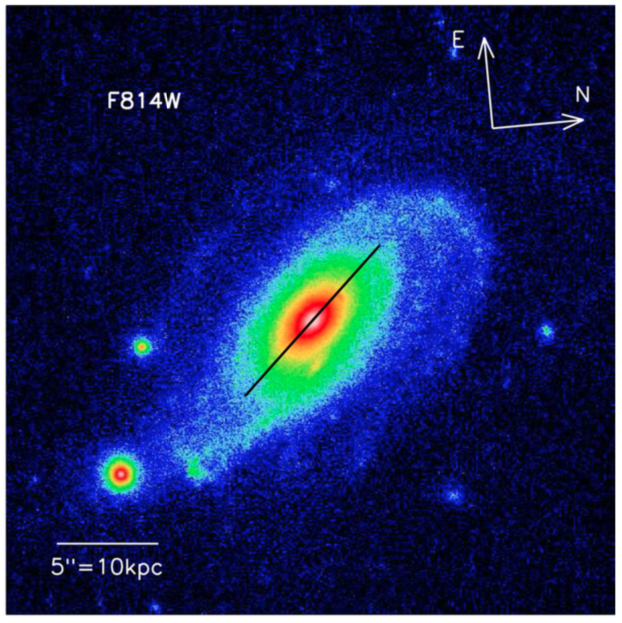
\includegraphics[width=0.45\columnwidth]{Kap2/J1331.png}
  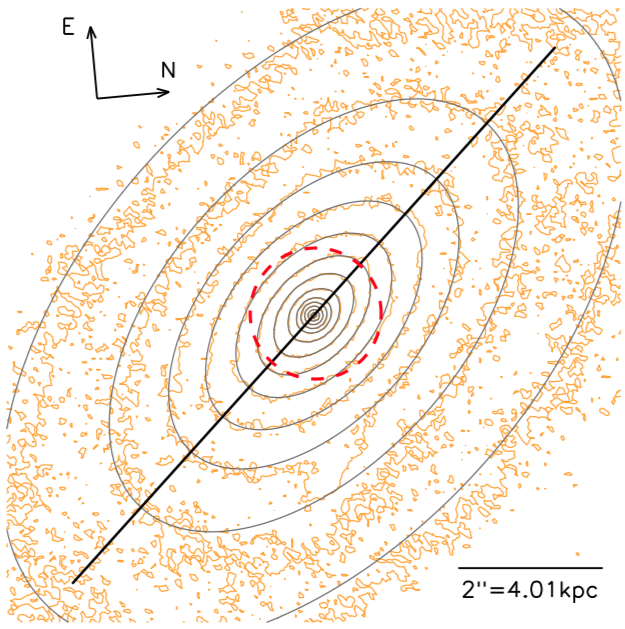
\includegraphics[width=0.45\columnwidth]{Kap2/MGE_1.png}
  \caption{Distribución de brillo superficial  por medio de la Expansión Multi-Gaussiana (MGE) donde se muestran los contornos de iso-densidad (derecha). Las líneas grises son la convolución de MGE con la PSF La línea negra corresponde a la orientación en el ángulo de posición de la galaxia espiral SDSS J1331+3628 (izquierda). Tomado de \cite{TR16}  }
  \label{fig:Fi4}
\end{figure}


\subsection{CAULDRON}

El algoritmo CAULDRON (Combined Lensing and Dynamics Analysis) es un marco en el cual se realiza un análisis auto consistente para unificar los resultados de obtener la distribución de masa con lente gravitacional y dinámica estelar. \cite{2007ApJ...666..726B}









\chapter{Lentes gravitacionales}

\section{Consideraciones cosmológicas}

De acuerdo a la cosmología observacional, los modelos de mundo uniforme estándar pueden ser descritos por los siguientes parámetros \cite{2008gafo.book.....L}:\\

\textbf{La constante de Hubble} $H_0$ describe la razón de expansión presente del universo:

$$ H_0 = \left( \frac{\dot{a}}{a} \right)_{t_0} = \dot{a}(t_0),$$

\textbf{el parámetro de desaceleración} $q_0$ describe la desaceleración adimensional presente del universo:

$$ q_0 = -\left( \frac{\ddot{a} a }{\dot{a}^2} \right)_{t_0} = -\frac{\ddot{a}(t_0)}{H_0^2}, $$

y \textbf{el parámetro de densidad} $\Omega_0$ es la razón de la densidad de masa-energía presente del universo $\rho_0$ a la densidad crítica $\rho_c$:

$$\Omega_0 = \frac{\rho_0}{\rho_c} = \frac{8\pi G\rho_0}{3H_0^2}, $$

con $$ \rho_c = \frac{3H_0^2}{8\pi G}. $$

Otros parámetros útiles en términos de materia barionica y no barionica son:\\

y \textbf{El parámetro de densidad de los campos de vacío}, o la energía oscura:

\begin{eqnarray}
\Omega_{\Lambda} = \frac{8\pi G \rho_v}{3 H_0^2} = \frac{\Lambda}{3H_0^2},
\end{eqnarray}

con $\Lambda$ la cosntante cosmológica.\\

Éstos parámetros no son independientes, se tienen las siguientes dos ecuaciones:

$$ \kappa \left( \frac{c}{H_0} \right)^2 = (\Omega_0 + \Omega_{\Lambda}) - 1, $$

$$ q_0 = \frac{\Omega_0}{2} - \Omega_{\Lambda}. $$

La medida de distancias dependientes del \emph{redshift} son determinadas por la geometría y dinámica del Universo. Los parámetros $\Omega_{0} , \Omega_{\Lambda}$ pueden ser determinados directamente, pues si se conoce con precisión una distancia $D$ a un objeto por una técnica independiente del \emph{redshift}, se puede observar el comportamiento en gráficas como $D$ vs. $z$. Los parámetros cosmológicos también pueden ser probados por las propiedades de la materia oscura mediante técnicas de dinámica galáctica vista anteriormente y por el efecto de lentes gravitacionales como se detalla en este capítulo.\\

%La constante de Hubble es: $ H_0 = 70 \hspace{3mm} km s^{-1}  Mpc^{-1} $. 

Los parámetros cosmológicos son determinados por observaciones de objetos distantes tal como galaxias, cúmulos de galaxias y cuasares que son soportados por la Radiación cósmica de fondo de microondas  (CMB por sus siglas en inglés \emph{Cosmic Microwave Background Radiation}) y la distribución a gran escala de galaxias. Los siguientes valores para los parámetros cosmológicos son para un modelo plano $\Lambda$CDM con una ley de potencias simple del espectro de potencia (la constante de Hubble $H$ está reescalada en $h$ adimencional):

\begin{eqnarray}
 h &=& 0.73_{-0.03}^{+0.007} \\
 \omega_B = \Omega_B h^2 &=& 0.0223_{0.0009}^{0.0007} \\
  \omega_D = \Omega_D h^2 &=& 0.127_{0.0013}^{0.007}
\end{eqnarray}

con $\Omega_D$ el parámetro de densidad de materia oscura fría y  $\Omega_B$ el parámetro de densidad de Bariones. Para los cuales $\Omega_B + \Omega_D + \Omega_{\Lambda} +\Omega_k= 1$. Los datos son tomados de WMAP (Wilkinson Microwave Anisotropy Probe)\footnote{Ver: http://lambda.gsfc.nasa.gov/product/map/dr2/parameters\_info.cfm}.




\subsection{Distancia diametral angular}

Si un objeto tiene tamaño propio $L$, la luz toma un intervalo $\delta t$ y de la condición $ds = 0 (dr = s\theta = 0)$ se tiene que:

$$c \delta t = R(t_1) r \delta $$ 

con $t_1$ el tiempo de emisión y $\delta$ la separación angular , la distancia diametral angular está definida por:

$$ d_A = R(t_1) r $$

\begin{figure}
\centering%
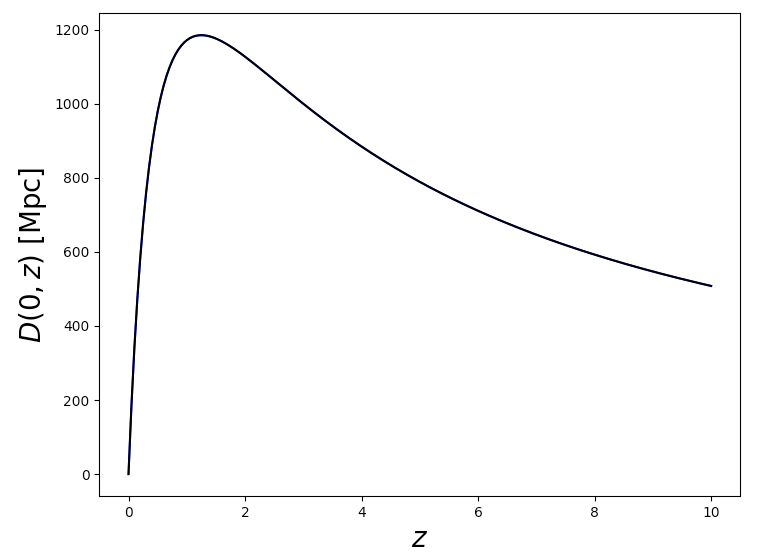
\includegraphics[width=0.9\columnwidth]{Kap3/d_A.png}%
\caption{Relación de la distancia diametral respecto a \emph{redshift}.}
\label{fig:grav_lens_1}
\end{figure}

La distancia diametral angular es función del \emph{redshift} $z$. En el caso de un universo plano se tiene \cite{CA10}:

\begin{equation}
D(0, z_s) = \frac{c}{H_0 (1+z_s)} = \int_0^{z_s} \frac{dz}{(1+z)\sqrt{\Omega_{mo}(1+z) + \Omega_{R0}(1+z)^2 +\Omega_{Q0}(1+z)^3 +\Omega_{k0} }}.
\end{equation}

La ecuación diferencial que relaciona la distancia $r$ a una fuente con \emph{redshift, z} está dada por:

\begin{eqnarray}
\left [  \Omega_{m0}z + 1 + \Omega_{Q0}(1+z)^{m-2} \left ( 1-\frac{1}{(1+z)^{m-2} } \right ) \right ] \frac{d^2 r}{d z^2} &+& \\
\frac{1}{1+z} \left [ \frac{7 \Omega_{m0}z }{2} + \frac{\Omega_{m0}}{2} + 3 + \Omega_{Q0} (1+z)^{m-2} \left ( \frac{m+4}{2} - \frac{3}{(1+z)^{m-2}} \right ) \right ] \frac{d r}{d z} &+& \\
\frac{3}{2(1+z)^4} \left [ \vec{\alpha} \Omega_{m0} (1+z)^3 + \vec{\alpha}_x \frac{m}{3} \Omega_{Q0} (1+z)^m \right ] r &=& 0
\end{eqnarray}

con condiciones de frontera dadas por:

\begin{eqnarray}
r(\textrm{z}_0, z_0) &=& 0 \\
\frac{dr \textrm{z}_0, z}{d z} |_{z = z_0} &=& H_0 \frac{dr_p(z_0)}{d z} |_{z = z_0} \\
    & = & \frac{1}{(1+z_0)^2 \sqrt{\Omega_{m0}z_0 + 1 + \Omega_{Q0}(1+z)^{m-2} \left [ 1-\frac{1}{(1+z_0)^{m-2} } \right ]  }}
\end{eqnarray}

%\cite{HU14}

\section{La ecuación de lente}

La ecuación de lente es la relación entre la posición angular de una fuente no afectada por el efecto de lente gravitacional, y la posición de sus imágenes si los rayos de luz que emanan de la fuente son perturbados por el campo gravitacional.\\

La masa total de un sistema estelar o de un cúmulo de galaxias puede ser encontrado a través del formalismo desarrollado como si ésta masa se comportara como lente gravitacional, donde el potencial gravitacional $\Psi$ correspondiente a la lente \emph{M} describe la deflexión  de los rayos de luz desde una fuente \emph{S} (tomado como una galaxia) hasta un observador \emph{O}, como se muestra en la Figura (\ref{fig:grav_lens_1}).\\

\begin{figure}
\centering%
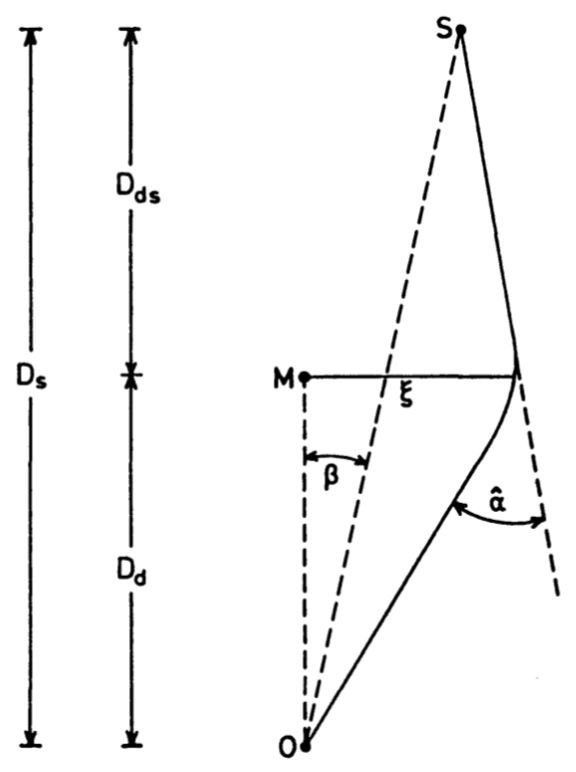
\includegraphics[width=0.4\columnwidth]{Kap3/grav_lens_1.png}%
\caption{Esquema de lente gravitacional \cite{SN92}.}
\label{fig:grav_lens_1}
\end{figure}

Las distancias diametrales angulares observador-lente $D_d$, observador-fuente $D_s$ y lente-fuente $D_{ds}$ relacionan el potencial de deflexión proyectado a lo largo de la línea de visión:

\begin{equation}
\Psi ( \bm{\theta}) = \frac{D_{ds}}{D_{d} D_{s}} \frac{2}{c^2} \int \Phi ( \bm{r} = D_d \bm{\theta}, z) dz,
\end{equation}

con los vectores de dos dimensiones $\bm{\theta} \equiv (x', y')$ en el plano del cielo, y $\bm{\beta} \equiv (x_s', y_s')$ dado por la relación vectorial:

\begin{equation}
\bm{\beta} = \bm{\theta}_i - \nabla_{\theta} \Psi (\bm{\theta}) |_{\bm{\theta}_i}
\end{equation}


La masa del sistema estelar, encerrada en el radio de Einstein $R_{ein}$ está dada por:

\begin{equation}
M_{ein} \equiv M(<R_{ein}) = \pi \Sigma_{crit}R_{ein}^2
\end{equation}

donde la densidad crítica $\Sigma_{crit}$ es la densidad de masa que ...

\begin{equation}
\Sigma_{crit} \equiv \frac{c^2}{4 \pi G} \frac{D_s}{D_d D_{ds}}
\end{equation}


\section{Modelos de lente}

\subsection{Modelos libres de escala}

Los modelos libres de escala con ley de potencias, con una disminución arbitraria en la parte exterior de la curva de rotación, tienen la característica que sus isofotas tienen la misma forma en cada radio y están completamente descritas por una función de forma $G(\theta)$. Ésta función depende solo del ángulo de posición $\theta$ con respecto al eje mayor. Esta descripción permite expresar el potencial de deflexión de la luz $\phi$ y la convergencia $\kappa$ proporcionales a $r$:

\begin{eqnarray}
\kappa &=& \frac{1}{2} G(\theta) r{\beta-2}, \\
\phi &=& r^{\beta} F(\theta)
\end{eqnarray}

en el plano de la lente. La potencia $\beta$ está restringida a $0<\beta<2$ para modelos galácticos , siendo $\beta=1$ en caso de una curva de rotación plana.\\

Bajo este modelo la función de forma $G(\theta)$ puede ser escrita como:

\begin{equation}
\label{G_theta}
G(\theta) = \beta^2 F(\theta) + F''(\theta), 
\end{equation}

donde dada una función $G(\theta)$ se puede hallar $F(\theta)$ solucionando la ecuación diferencial. Esto permite encontrar el potencial libre de escala correspondiente a un conjunto de contornos de igual densidad libres de escala \cite{EV03}.


\subsubsection{Método de expansión en serie de Fourier}

Las funciones $F(\theta), G(\theta)$ son periódicas, entonces se pueden expandir en serie de Fourier. Entonces expandiendo la función $F(\theta)$ y usando la ecuación (\ref{G_theta}):

\begin{eqnarray}
\label{Fourier_F}
F(\theta) &=& \frac{a_0}{2} + \sum_{k=1}^{\infty} \left[ a_k cos(k \theta) + b_k sin (k \theta) \right],\\
G(\theta) &=& \frac{a_0 \beta^2}{2} + \sum_{k=1}^{\infty} \left[ a_k (\beta^2-k^2) cos(k \theta) + b_k (\beta^2-k^2) sin (k \theta) \right],
\end{eqnarray}

Los coeficientes en la serie de Fourier debe satisfacer la condición $G(\theta) \geq 0$ para todo $\theta$ y obtener la densidad superficial positiva. 

\subsubsection{Las posiciones de las imágenes y los flujos}

Usando coordenadas polares en el plano de la imagen, la ecuación de lente tiene la forma:

\begin{eqnarray}
\xi & = & x - \frac{\partial \phi}{\partial x}, \\
\eta & = &  y - \frac{\partial \phi}{\partial y}
\end{eqnarray}



\begin{eqnarray}
\label{lens_equation_power_law}
\xi & = & r cos(\theta) - r^{\beta-1}\left[ \beta cos(\theta)F(\theta) - sin(\theta) F'(\theta)  \right] , \\
\eta & = &  r sin(\theta) - r^{\beta-1}\left[ \beta sin(\theta)F(\theta) - cos(\theta) F'(\theta)  \right]
\end{eqnarray}

donde $F(\theta)$ y $F'(\theta)$ están dadas por la serie de Fourier (\ref{Fourier_F}).\\

\subsubsection{Ajuste al modelo}

A continuación se describe el procedimiento para encontrar el valor de la potencia $\beta$, y una vez obtenido, la ecuación resultante es lineal y puede ser resuelta por métodos numéricos para la posición $(\xi, \eta)$ y los parámetros de Fourier $(a_k, b_k)$ dada una imagen observada en la posición

\begin{eqnarray}
x_i' &=& R_i' cos (\theta_i'),\\
y_i' &=& R_i' sin (\theta_i').
\end{eqnarray}
 
Se requiere minimizar la distancia entre \textbf{$\theta_{0i}$} y el modelo de lente predicho \textbf{$\theta_{pi}$} Para evitar resolver la ecuación de lente (\ref{lens_equation_power_law}) para  \textbf{$\theta_{pi}$}, se usa el tensor de magnificación para aproximar 

 

$$\bm{\theta} \approx \frac{\partial \bm{\theta}}{\partial \bm{\beta} } \bm{\beta} =  \bm{M} \bm{\beta},  $$

así entonces el modelo de mejor ajuste es tal que minimiza \cite{TR16} la cantidad

\[
\chi_{lens}^2 = \sum_{i} \left |
\begin{bmatrix}
    1/\Delta x & 0 \\
    0 & 1/\Delta y
\end{bmatrix}
\left ( \bm{\theta}_{pi} - \bm{\theta}_{0i} \right ) \right |^2 \approx \sum_{i} \left |
\begin{bmatrix}
    1/\Delta x & 0 \\
    0 & 1/\Delta y
\end{bmatrix}
 \bm{M}|_{\bm{\theta} = \bm{\theta}_{0i}} 
\begin{bmatrix}
    \xi_s' - \overline{\xi_s'} \\
    \eta_s' - \overline{\eta_s'}
\end{bmatrix}
 \right |^2 ,
\]

donde $(\Delta x, \Delta y)$ son los errores de medición de las posiciones $\bm{\theta}_{0i}$. Y $\bm{M}|_{\bm{\theta} = \bm{\theta}_{0i}}$ es el tensor de magnificación y $(\overline{\xi_s'}, \overline{\eta_s'})$ la posición de la fuente de acuerdo a la posición de la lente. \\

Por lo tanto la cantidad a minimizar es \cite{TR16}:

\begin{equation}
\chi^2 = \chi_{lens}^2 + \chi_{shape}^2,
\end{equation}

con $\chi_{shape}^2$ un término para restringir la forma de la distribución de masa a una elipse. Para encontrar la potencia $\beta$ se necesitan las razones de flujos para las imágenes.\\

En \cite{TR16} se encontró el modelo de lente como el mejor ajuste a las posiciones de lente de la imagen siguiendo el modelo libre de escala. En la figura \ref{fig:lens_model} se ilustra el resultado.

\begin{figure}
\centering%
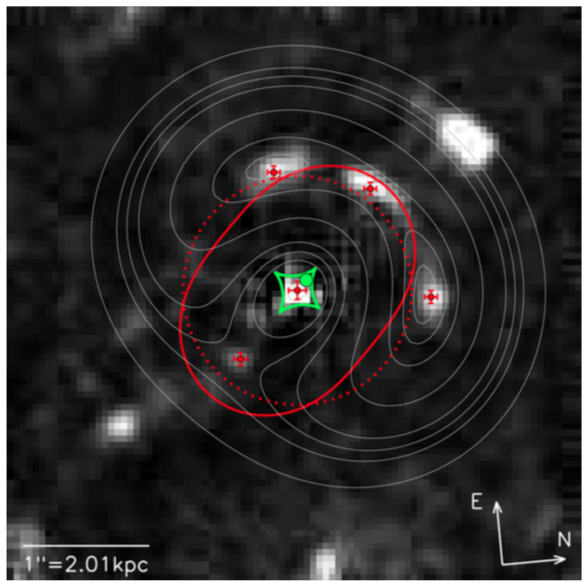
\includegraphics[width=0.8\columnwidth]{Kap3/lens_model.png}%
\caption{Modelo de lente para la lente en el centro de la galaxia espiral SDSS J1331+3628. La línea roja punteada es el círculo en el radio de Einstein, en la línea sólida roja se muestra la curva crítica y la caustica en la línea verde (tomado de \cite{TR16})}
\label{fig:lens_model}
\end{figure}


\begin{equation}
-----------------------------
\end{equation}





\chapter{Métodos de dinámica galáctica y lentes gravitacionales para estimación de masas}

http://adsabs.harvard.edu/abs/2007ApJ...666..726B


\chapter{Cap\'{\i}tulo ...}
...
\chapter{Conclusiones y recomendaciones}
\section{Conclusiones}
Las conclusiones constituyen un cap\'{\i}tulo independiente y presentan, en forma l\'{o}gica, los resultados de la tesis  o trabajo de investigaci\'{o}n. Las conclusiones deben ser la respuesta a los objetivos o prop\'{o}sitos planteados. Se deben titular con la palabra conclusiones en el mismo formato de los t\'{\i}tulos de los cap\'{\i}tulos anteriores (T\'{\i}tulos primer nivel), precedida por el numeral correspondiente (seg\'{u}n la presente plantilla).\\

\section{Recomendaciones}
Se presentan como una serie de aspectos que se podr\'{\i}an realizar en un futuro para emprender investigaciones similares o fortalecer la investigaci\'{o}n realizada. Deben contemplar las perspectivas de la investigaci\'{o}n, las cuales son sugerencias, proyecciones o alternativas que se presentan para modificar, cambiar o incidir sobre una situaci\'{o}n espec\'{\i}fica o una problem\'{a}tica encontrada. Pueden presentarse como un texto con caracter\'{\i}sticas argumentativas, resultado de una reflexi\'{o}n acerca de la tesis o trabajo de investigaci\'{o}n.\\
\begin{appendix}
\chapter{Anexo: Potencial gravitacional de un disco delgado}\label{AnexoA}
El potencial de un disco delgado en la región exterior del mismo, con altura mucho menor que el radio del disco, y simetría axial, se realiza separación de variables.

Expresando la \textbf{ecuación de Laplace} en coordenadas cilíndricas $(R, \phi, z)$ para este sistema con simetría axial y simetría respecto el plano $z=0$, $\Phi = \Phi(R, z) = \Phi(R, -z)$:

\begin{equation}
\label{laplace_eq_disk}
\frac{1}{R} \frac{\partial }{\partial R}  \left ( R \frac{\partial \Phi }{\partial R}  \right ) + \frac{\partial^2 \Phi }{\partial z^2}  = 0,
\end{equation}

donde el potencial es

$$ \Phi(R,z) = J(R) Z(z). $$

Se tiene que la ecuación (\ref{laplace_eq_disk}) se puede escribir en términos de las funciones radial $J(R)$ y de altura $Z(z)$:

\begin{eqnarray}
   Z(z) \frac{1}{R} \frac{1}{R} \frac{d}{R} \left( R \frac{d J(R)}{R} \right) + J(R) \frac{d^2}{d z^2} Z(z) &=& 0, \\
    \frac{1}{JR} \frac{d}{R}  \left( R \frac{d J(R)}{R} \right) = -\frac{1}{Z}  \frac{d^2}{d R^2} Z(z) &=& -k^2.  \\
\end{eqnarray}

Entonces  la ecuación que depende de $z$ , tiene solución:
$$  \frac{d^2}{d z^2} Z(z)  -k^2 Z(z) = 0    \hspace{1cm}, \hspace{1cm} Z=A e^{kz} + B e^{-kz} $$







\chapter{Anexo: Nombrar el anexo B de acuerdo con su contenido}
A final del documento es opcional incluir \'{\i}ndices o glosarios. \'{E}stos son listas detalladas y especializadas de los t\'{e}rminos, nombres, autores, temas, etc., que aparecen en el mismo. Sirven para facilitar su localizaci\'{o}n en el texto. Los \'{\i}ndices pueden ser alfab\'{e}ticos, cronol\'{o}gicos, num\'{e}ricos, anal\'{\i}ticos, entre otros. Luego de cada palabra, t\'{e}rmino, etc., se pone coma y el n\'{u}mero de la p\'{a}gina donde aparece esta informaci\'{o}n.\\

\chapter{Anexo: Nombrar el anexo C de acuerdo con su contenido}
MANEJO DE LA BIBLIOGRAF\'{I}A: la bibliograf\'{\i}a es la relaci\'{o}n de las fuentes documentales consultadas por el investigador para sustentar sus trabajos. Su inclusi\'{o}n es obligatoria en todo trabajo de investigaci\'{o}n. Cada referencia bibliogr\'{a}fica se inicia contra el margen izquierdo.\\

La NTC 5613 establece los requisitos para la presentaci\'{o}n de referencias bibliogr\'{a}ficas citas y notas de pie de p\'{a}gina. Sin embargo, se tiene la libertad de usar cualquier norma bibliogr\'{a}fica de acuerdo con lo acostumbrado por cada disciplina del conocimiento. En esta medida es necesario que la norma seleccionada se aplique con rigurosidad.\\

Es necesario tener en cuenta que la norma ISO 690:1987 (en Espa\~{n}a, UNE 50-104-94) es el marco internacional que da las pautas m\'{\i}nimas para las citas bibliogr\'{a}ficas de documentos impresos y publicados. A continuaci\'{o}n se lista algunas instituciones que brindan par\'{a}metros para el manejo de las referencias bibliogr\'{a}ficas:\\

\begin{center}
\centering%
\begin{tabular}{|p {7.5 cm}|p {7.5 cm}|}\hline
\arr{Instituci\'{o}n}&Disciplina de aplicaci\'{o}n\\\hline%
Modern Language Association (MLA)&Literatura, artes y humanidades\\\hline%
American Psychological Association (APA)&Ambito de la salud (psicolog\'{\i}a, medicina) y en general en todas las ciencias sociales\\\hline
Universidad de Chicago/Turabian &Periodismo, historia y humanidades.\\\hline
AMA (Asociaci\'{o}n M\'{e}dica de los Estados Unidos)&Ambito de la salud (psicolog\'{\i}a, medicina)\\\hline
Vancouver &Todas las disciplinas\\\hline
Council of Science Editors (CSE)&En la actualidad abarca diversas ciencias\\\hline
National Library of Medicine (NLM) (Biblioteca Nacional de Medicina)&En el \'{a}mbito m\'{e}dico y, por extensi\'{o}n, en ciencias.\\\hline
Harvard System of Referencing Guide &Todas las disciplinas\\\hline
JabRef y KBibTeX &Todas las disciplinas\\\hline
\end{tabular}
\end{center}

Para incluir las referencias dentro del texto y realizar lista de la bibliograf\'{\i}a en la respectiva secci\'{o}n, puede utilizar las herramientas que Latex suministra o, revisar el instructivo desarrollado por el Sistema de Bibliotecas de la Universidad Nacional de Colombia\footnote{Ver: www.sinab.unal.edu.co}, disponible en la secci\'{o}n "Servicios", opci\'{o}n "Tr\'{a}mites" y enlace "Entrega de tesis".

\end{appendix}
\addcontentsline{toc}{chapter}{\numberline{}Bibliograf\'{\i}a}
\bibliographystyle{plaindin_esp}
\bibliography{BibliMSc}
\end{document}